%Version 3.1 December 2024
% See section 11 of the User Manual for version history
%   
%%%%%%%%%%%%%%%%%%%%%%%%%%%%%%%%%%%%%%%%%%%%%%%%%%%%%%%%%%%%%%%%%%%%%%
%%                                                                 %%
%% Please do not use \input{...} to include other tex files.       %%
%% Submit your LaTeX manuscript as one .tex document.              %%
%%                                                                 %%
%% All additional figures and files should be attached             %%
%% separately and not embedded in the \TeX\ document itself.       %%
%%                                                                 %%
%%%%%%%%%%%%%%%%%%%%%%%%%%%%%%%%%%%%%%%%%%%%%%%%%%%%%%%%%%%%%%%%%%%%%

%%\documentclass[referee,sn-basic]{sn-jnl}% referee option is meant for double line spacing

%%=======================================================%%
%% to print line numbers in the margin use lineno option %%
%%=======================================================%%

%%\documentclass[lineno,pdflatex,sn-basic]{sn-jnl}% Basic Springer Nature Reference Style/Chemistry Reference Style

%%=========================================================================================%%
%% the documentclass is set to pdflatex as default. You can delete it if not appropriate.  %%
%%=========================================================================================%%

%%\documentclass[sn-basic]{sn-jnl}% Basic Springer Nature Reference Style/Chemistry Reference Style

%%Note: the following reference styles support Namedate and Numbered referencing. By default the style follows the most common style. To switch between the options you can add or remove “Numbered” in the optional parenthesis. 
%%The option is available for: sn-basic.bst, sn-chicago.bst%  
 
%%\documentclass[pdflatex,sn-nature]{sn-jnl}% Style for submissions to Nature Portfolio journals
%%\documentclass[pdflatex,sn-basic]{sn-jnl}% Basic Springer Nature Reference Style/Chemistry Reference Style
\documentclass[pdflatex,sn-mathphys-num,oneside]{sn-jnl}% Math and Physical Sciences Numbered Reference Style
\input{glyphtounicode}
\pdfgentounicode=1

\usepackage{graphicx}%
\usepackage{multirow}%
\usepackage{amsmath,amssymb,amsfonts}%
\usepackage{amsthm}%
\usepackage{mathrsfs}%
\usepackage[title]{appendix}%
\usepackage{xcolor}%
\usepackage{textcomp}%
\usepackage{manyfoot}%
\usepackage{booktabs}%
\usepackage{algorithm}%
\usepackage{algorithmicx}%
\usepackage{algpseudocode}%
\usepackage{listings}%
\usepackage{placeins}%
\usepackage{adjustbox}%
\usepackage{array}%
\usepackage{tabularx}%
\usepackage{enumitem}%
\usepackage{xurl}%
%%%%


%% as per the requirement new theorem styles can be included as shown below
\theoremstyle{thmstyleone}%
\newtheorem{theorem}{Theorem}%  meant for continuous numbers
%%\newtheorem{theorem}{Theorem}[section]% meant for sectionwise numbers
%% optional argument [theorem] produces theorem numbering sequence instead of independent numbers for Proposition
\newtheorem{proposition}[theorem]{Proposition}% 
%%\newtheorem{proposition}{Proposition}% to get separate numbers for theorem and proposition etc.

\theoremstyle{thmstyletwo}%
\newtheorem{example}{Example}%
\newtheorem{remark}{Remark}%

\theoremstyle{thmstylethree}%
\newtheorem{definition}{Definition}%

\raggedbottom
\geometry{bindingoffset=0mm,hcentering}
% ---------------- Layout-only fixes for float alignment and spacing ----------------
\setlength{\textfloatsep}{8pt plus 2pt minus 2pt}
\setlength{\floatsep}{6pt plus 2pt minus 2pt}
\setlength{\intextsep}{6pt plus 2pt minus 2pt}
\setlength{\abovecaptionskip}{2pt}
\setlength{\belowcaptionskip}{4pt}

\newlength{\journalfloatwidth}
\setlength{\journalfloatwidth}{0.92\linewidth}
% -------------------------------------------------------------------------------

\begin{document}

\title[Article Title]{FedFACS: A Fair Adaptive Client Selection Framework for Communication-Efficient Federated Learning}

% Anonymous blank author area
\author{\fnm{\rule{0pt}{5.2cm}}\sur{}}
%%==================================%%
%% Sample for unstructured abstract %%
%%==================================%%

\abstract{
Federated Learning (FL) is a distributed learning framework that enables clients to jointly optimize a common model through server coordination, while their local training data remain within their respective environments. Despite its privacy advantages, FL encounters significant challenges resulting from the participation of numerous clients having heterogeneous data during each training round. Consequently, this degrades accuracy, delays convergence, increases the communication overhead, and undermines fairness among participating clients. Hence, Client Selection (CS) has become essential for identifying the most beneficial clients for global model training. However, existing approaches often struggle to preserve model accuracy and fairness while limiting communication costs in the presence of non-Independent and Identically Distributed (non-IID) data. In response to these challenges, we introduce FedFACS (Federated Fair Adaptive Client Selection), a novel framework designed to handle data heterogeneity while improving fairness and training efficiency. FedFACS formulates client selection using a multi-objective fitness function combining the expected reduction in Kullback–Leibler (KL) divergence with a dynamic fairness baseline. In addition, we incorporate an uncertainty-aware penalty that mitigates the impact of local noise. Moreover, a control mechanism is introduced to adaptively balance utility and fairness in response to global convergence feedback. A dynamic cohort sizing mechanism was developed that identifies the optimal number of high-fitness clients needed for each round. Furthermore, we propose a stability-weighted aggregation method that aligns model aggregation with the stability criteria. Extensive experiments across multiple datasets under several data heterogeneous settings show that FedFACS achieves average improvements of 1.39\% in accuracy, 1.41\% in F1-score, and 0.44\% in recall, as well as 3.47\% fewer selected clients while maintaining comparable communication rounds, in addition to improving fairness by an average of 1.38\% in Jain's Fairness Index (JFI), relative to the best performing existing method, thereby enhancing performance and reducing communication overhead while ensuring fairness.
}

%%================================%%
%% Sample for structured abstract %%
%%================================%%

% \abstract{\textbf{Purpose:} The abstract serves both as a general introduction to the topic and as a brief, non-technical summary of the main results and their implications. The abstract must not include subheadings (unless expressly permitted in the journal's Instructions to Authors), equations or citations. As a guide the abstract should not exceed 200 words. Most journals do not set a hard limit however authors are advised to check the author instructions for the journal they are submitting to.
% 
% \textbf{Methods:} The abstract serves both as a general introduction to the topic and as a brief, non-technical summary of the main results and their implications. The abstract must not include subheadings (unless expressly permitted in the journal's Instructions to Authors), equations or citations. As a guide the abstract should not exceed 200 words. Most journals do not set a hard limit however authors are advised to check the author instructions for the journal they are submitting to.
% 
% \textbf{Results:} The abstract serves both as a general introduction to the topic and as a brief, non-technical summary of the main results and their implications. The abstract must not include subheadings (unless expressly permitted in the journal's Instructions to Authors), equations or citations. As a guide the abstract should not exceed 200 words. Most journals do not set a hard limit however authors are advised to check the author instructions for the journal they are submitting to.
% 
% \textbf{Conclusion:} The abstract serves both as a general introduction to the topic and as a brief, non-technical summary of the main results and their implications. The abstract must not include subheadings (unless expressly permitted in the journal's Instructions to Authors), equations or citations. As a guide the abstract should not exceed 200 words. Most journals do not set a hard limit however authors are advised to check the author instructions for the journal they are submitting to.}

\keywords{Federated learning, Client Selection, Communication-Efficient, Fairness}

%%\pacs[JEL Classification]{D8, H51}

%%\pacs[MSC Classification]{35A01, 65L10, 65L12, 65L20, 65L70}

\maketitle

\section{Introduction}\label{sec1}
Federated Learning (FL) establishes a distributed collaborative framework, where multiple devices are coordinated by a central server for joint model optimization, while each participant performs local training and maintains its data within its own environment throughout the training process, thus maintaining data privacy while reducing communication overhead. Consequently, FL has gained considerable attention in applications where data confidentiality is critical, including smart transportation, financial services, and healthcare (Shanmugarasa et al. 2023). Therefore, the global federated learning market is expected to grow significantly, rising from USD 133.1 million in 2023 to nearly USD 311.4 million by 2032. This growth corresponds to an estimated annual rate of 10.2\% and is associated with increasing investment and interest in privacy-preserving distributed learning technologies (Globe Newswire 2024).

In conventional federated learning, model training is organized into successive communication rounds coordinated by the server. At the beginning of each round, the latest global model is transmitted to all participating clients, which use the received model to conduct local training and subsequently return their updates to the coordinating server for aggregation. This cycle continues over successive rounds until the specified training accuracy threshold is reached (Kairouz et al. 2021), as depicted in Fig. 1. A major concern associated with FL is the communication overhead resulting from the repeated exchange of model parameters among participating clients and the coordinating server across successive training rounds. This overhead tends to increase as more clients join the federated network.

\begin{figure}[!htbp]
\centering
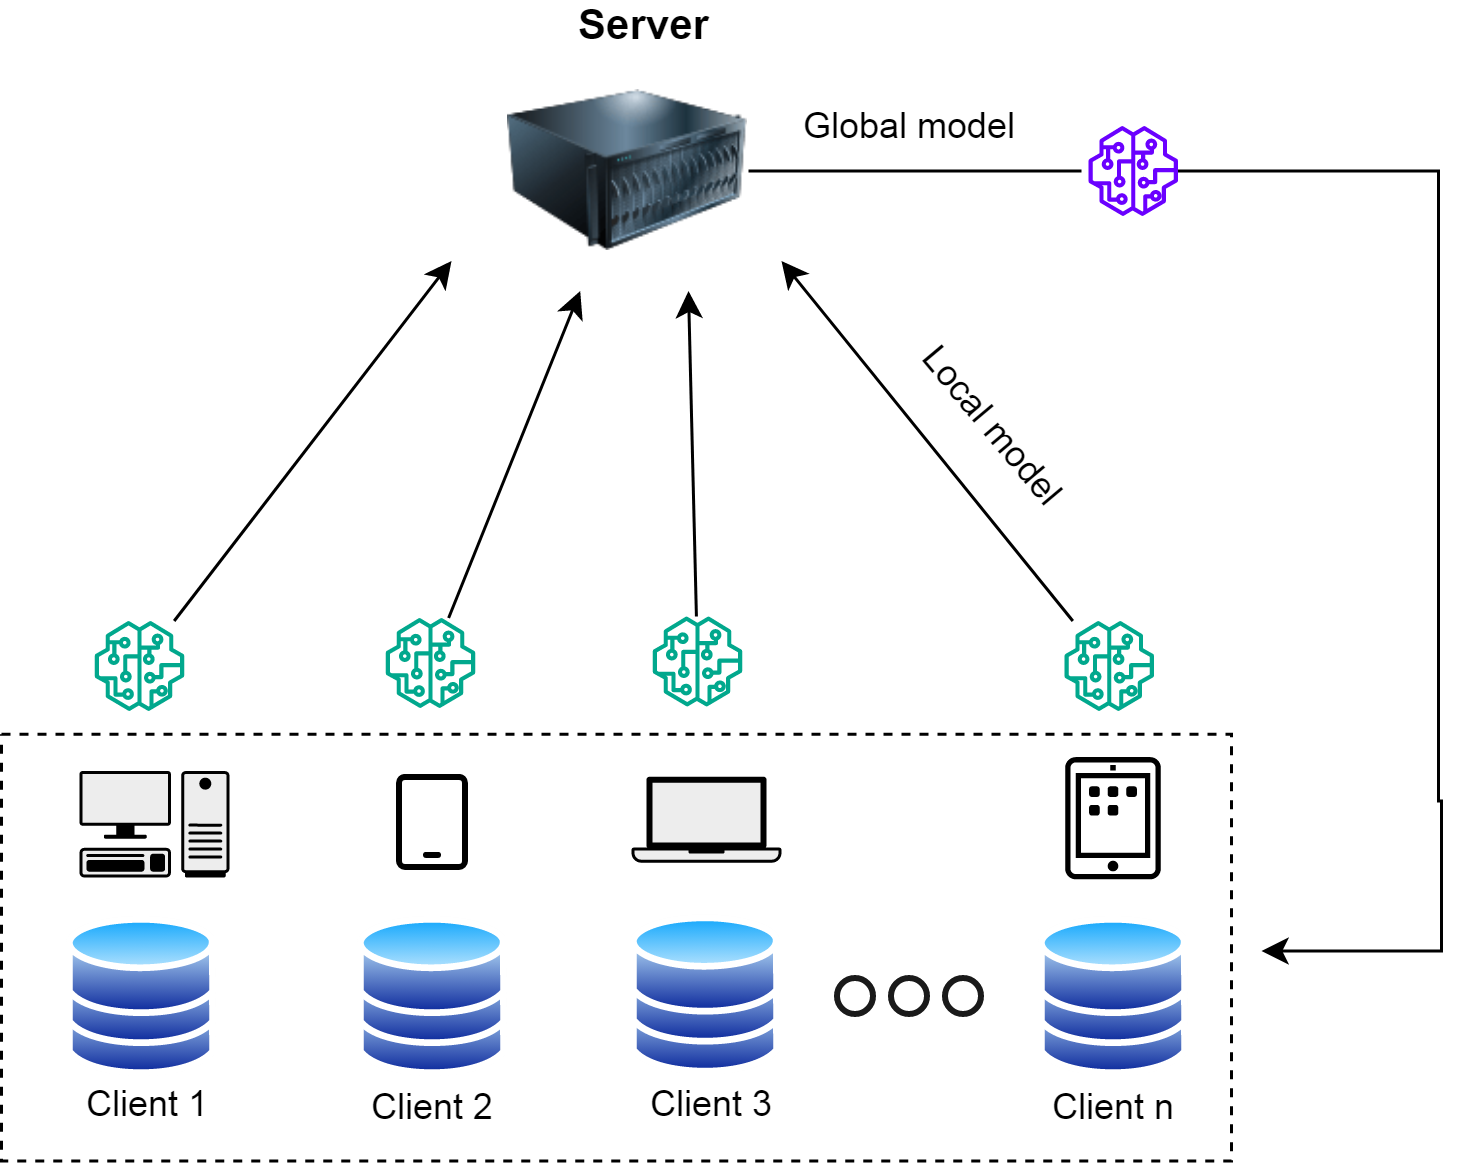
\includegraphics[width=0.85\textwidth]{figures/fig1.png}
\caption{Federated learning iterative process.}\label{fig:fl_arch}
\end{figure}

Moreover, the training process becomes more challenging when participating clients have different data distributions, dataset sizes, data quality, or computational capabilities. Such heterogeneity may introduce fairness issues, slow global convergence, and negatively impact the performance of the resulting global model (Kairouz et al. 2021; Khajehali et al. 2023; Mayhoub and Shami 2024; Fu et al. 2023; Wen et al. 2023).

Consequently, an effective client selection strategy is vital for identifying the most informative participants in each round contributes toward global model improvement, thereby limiting communication overhead (Asad et al. 2023), accelerating convergence, and enhancing performance. However, several client selection techniques rely on predefined participation ratios or fixed cohort sizes (Lai et al. 2021; Larsson et al. 2021). Such methods can result in the selection of participants that provide limited contributions to the global model. Other approaches are categorized as resource-based (Nishio and Yonetani 2019; Li et al. 2022), bandwidth-based (Cha et al. 2022; Ji et al. 2023), or correlation-based (Cho et al. 2022; Tang et al. 2021). However, most of these techniques fail to balance global and local factors, neglecting fair participation under non-IID data distributions. As a result, participants with larger datasets, better data quality, or stronger computational resources are repeatedly selected, while others remain idle for many rounds, which can bias the global model and affect generalization (Vucinich and Zhu 2023; Ayeelyan et al. 2025). Nonetheless, balancing performance and fairness in FL client selection under non-IID conditions is still an open challenge.

To overcome this limitation, we propose the Federated Fair Adaptive Client Selection (FedFACS) framework to harmonize the conflicts between fairness with predictive performance, communication efficiency, and convergence under diverse non-IID scenarios. FedFACS introduces a multi-dimensional selection fitness score that prioritizes clients offering the highest contribution to global model by leveraging three core factors: utility, fairness, and uncertainty penalty. Client utility is quantified by estimating its potential contribution to the global model through the expected decrease in KL divergence across local and global predictive distributions (Kullback and Leibler 1951). The uncertainty penalty is estimated using the variance of KL divergence measured across multiple mini-batches for each client. Fairness is quantified using normalized idle rounds, dynamically determined by the server, thereby preventing client domination (Shi et al. 2024; Xu et al. 2024). Moreover, FedFACS balances utility and fairness using a control mechanism inspired by the Lyapunov control law (Chaudhari et al. 2002). The number of clients selected for aggregation (cohort size) is adaptively updated at every round in response to the current global model loss. Furthermore, the client contributions are quantified using stability score which is used to adaptively weight global model aggregation. The efficacy of FedFACS is demonstrated through rigorous evaluations across four benchmark datasets, outperforming competitive FL baselines across different data distribution settings. The key contributions of the proposed approach are summarized as follows:
\begin{enumerate}[label=\arabic*-]
\item Multi-Objective Fitness Function for Fair Adaptive Client Selection: We propose an adaptive client selection fitness function integrating KL-divergence-based client utility, an uncertainty penalty to improve robustness, and a dynamic fairness score for fair participation. Furthermore, the convergence progress of the global federated model guides the adjustment of fitness scores and determines the cohort size, thereby specifying the number of top-ranked clients selected for model aggregation in each training round. Specifically, the cohort size increases during convergence stagnation to encourage exploration and decreases during stable convergence under non-IID data settings to improve communication efficiency.

\item Adaptive control of the utility and fairness: We introduce a convergence-aware control parameter that dynamically balances utility and fairness for each client during training rounds according to the convergence behavior of the global model. Thus, the framework adjusts the relative weighting of fairness and utility based on the current convergence state.

\item Stability-weighted aggregation method: we present a stability-weighted aggregation scheme that adaptively adjusts the weight of the selected clients' local models during aggregation by leveraging their stability scores, thereby enhancing global accuracy, training robustness, and convergence speed.

\item We perform experimental evaluation using four benchmark datasets (MNIST, FMNIST, CIFAR10, and COVID-19) across diverse data heterogeneity conditions. The evaluation demonstrates improvements over existing federated learning methods in accuracy, communication efficiency, and fairness.
\end{enumerate}




\section{Related Works}
\label{sec2}

This section discusses prior work in federated learning, which addresses client selection, communication efficient optimization, aggregation, and fairness-aware techniques.

\subsection{Classical Federated Learning}

Over recent years, FL has gained considerable attention across numerous areas, such as healthcare, edge computing, finance, and computer vision (Ahmed and Alabi 2024; Darzi et al. 2024; Khan et al. 2024; Li et al. 2016). In computer vision domain, FL has shown effectiveness across multiple tasks, including image classification and recognition. FL faces two major challenges which are data heterogeneity and communication overhead. These challenges affect model performance. Consequently, there is a critical need for developing an optimized FL framework to overcome these challenges.

FedAvg acts as a simple and communication-efficient baseline for FL by averaging updates collected from participating clients to construct a shared global model. However, FedAvg struggles under non-IID data, which degrades performance and biases the global model. In addition, it ignores fairness (McMahan et al. 2017). Li et al. (2020) presented FedProx, which utilizes a proximal term to ensure stable local training and support faster convergence across clients with heterogeneous data distributions, although it introduces additional computational overhead. The SCAFFOLD approach proposed by Karimireddy et al. (2020) accelerates convergence through control variates that reduce the drift between server and client parameter updates. Nevertheless, it increases communication overhead as well as failing under highly heterogeneous data conditions, while FedAdam (Reddi et al. 2021) is an adaptive optimization approach that utilizes an adaptive server-side optimizer to enhance convergence. However, it raises server-side computation cost and does not address the fairness issue. Furthermore, FedNova (Wang et al. 2020) improves the convergence rate by eliminating objective inconsistency through normalizing local updates before aggregation, which enhances fairness. However, it does not address the impact of a large number of participants on communication cost under non-IID scenarios. 

\subsection{Modern Client Selection and Model Aggregation}

Classical federated learning assumes that each client possesses datasets of identical data and quality, as well as homogeneous hardware and network resources. Practically, participants have heterogeneous systems and data, which introduces many challenges, including performance degradation affecting the global model's accuracy and convergence rate. Moreover, for scalability and communication-efficiency, transmitting updates from all clients in every training round is impractical.


Numerous studies have proposed client selection methods, including random, communication-based, utility-based, correlation-based, and resource-based selection (Ayeelyan et al. 2025). In random selection methods, a fixed client count is chosen in each training round. However, these approaches suffer from restricted adaptability, inefficient convergence, and a lack of heterogeneous data awareness. Communication-based client selection methods aim to reduce latency and communication overhead. Li et al. (2024) proposed a performance-aware weight decay mechanism that utilizes historical model performance to adaptively control the number of participants, enhancing global model accuracy and decreasing communication costs. Tsouvalas et al. (2024) introduced a communication efficient algorithm named FedCompress, which enhances communication-efficiency by compressing the model while preserving model accuracy through dynamic clustered weighting. However, its beneficial effects may be restricted under strongly heterogeneous data distribution. Vanthang et al. (2025) proposed a utility-based client sampling framework that integrates fog computing with federated learning. The framework selects the most informative clients according to their gradients and reduces data transmission by adaptively adjusting selection thresholds under data heterogeneous scenario. Lai et al. (2021) developed the Oort client selection framework, which computes a utility score defined by three key factors: training time, local loss, and the client's past selection count. Cho et al. (2022) addressed communication efficiency through the Power-of-Choice strategy by prioritizing clients with high loss in every training round to accelerate global convergence. Ye et al. (2025) proposed an attention-based selection approach that enhances accuracy while minimizing communication overhead by adopting a “later-is-better” concept, where the client selection process ranks participants using their estimated contribution together with their alignment with the global model during each communication round. Zhai et al. (2024) developed an efficient approach for client selection that selects participants according to their evaluated quality. This approach employs a Multi-Armed Bandit (MAB) metric to evaluate client quality using two factors: individual contribution and correlation across clients. Consequently, the method accelerates convergence while enhancing global model accuracy. DivFL (Balakrishnan et al. 2022) is correlation-based selection method that improves convergence speed and performance by choosing the clients according to their gradient information. Nishio and Yonetani (2019) introduced a resource-based approach for selecting clients, considering clients’ data size, bandwidth, computational and communication capabilities to estimate client’s training time. To improve convergence, the server selects clients that are able to transmit their updates within a specified time. Liu et al. (2025) introduced AHIBCS, an approach designed to improve FL performance when data is non-identically distributed by leveraging both current and historical client behavior. The proposed method considers both the current training status and historical information of clients through an adaptive threshold mechanism. Based on the variation of local loss values, the algorithm dynamically switches between two client selection strategies: a loss-based strategy that prioritizes clients with higher losses to accelerate convergence, and a diversity-based strategy that selects clients with more diverse model updates to improve model generalization.

Model aggregation is performed after each communication round, where the selected client updates are aggregated at the server to produce the global model. Classical federated aggregation methods determine client weights according to their local dataset sizes (Ayeelyan et al. 2025; Zhai et al. 2024). The approach proposed by Ji et al. (2019) utilized trainable attention scores to weight local updates during global model aggregation. Furthermore, Wu et al. (2021) quantified client utility by measuring the directional alignment of local update vectors with the global optimization direction. These quantified values determine the weights assigned to each local update during every aggregation round. However, both approaches in (Ji et al. 2019; Wu et al. 2021) introduced an additional computational complexity and suppress rare informative features from clients possessing heterogeneous data. Zhai et al. (2024) introduced a dynamic aggregation method, which adaptively assigns weights according to the quality of the selected participants to improve model robustness and convergence.  


\subsection{Fairness-Based Client Selection}

Fairness in FL should aim to provide all clients with a fair opportunity to contribute during training. (Huang et al. 2024). Under non-IID conditions, a challenge arises from over exploiting high-contributing clients while under exploring underrepresented clients, leading to a biased global model that favors the repeatedly selected clients. Moreover, equal clients’ participation frequency affects the global model performance. Therefore, adaptive fairness mechanisms should be developed to balance exploitation (training with well-performing clients) and exploration (training with low-performing clients) to ensure fair participation (Bouzamoucha et al. 2025; Mukhtiar 2025; Mukhtiar et al. 2025; Zhang et al. 2022). Numerous approaches address fairness in federated learning from different perspectives.  


Huang et al. (2020) ensured fairness by selecting suitable clients utilizing a client selection method. However, fairness was not guaranteed, as the approach quantifies random selection probability. Song et al. (2022) developed a fairness-constrained reputation method to achieve a balance between client participation frequency and reputation in FL. Chaudhury et al. (2024) proposed a veto core approach to prevent client domination, preventing group deviation. However, this technique introduces significant communication and computational burdens. Wang et al. (2023) developed an entropy-based framework that balances fairness with global model accuracy. Shi et al. (2023) introduced a Lyapunov-based client selection approach, where the selection score depends on client reputation, participation frequency and Shapley value. Moreover, this approach allows clients to redeem their reputation to ensure fair participation and adjust their selection scores. However, it comes with computational overhead. Although multiple studies in FL have demonstrated the benefits of fair client participation, mainly in balancing exploitation and exploration under non-IID environments. Nevertheless, the problem of balancing fairness and global model performance while reducing communication cost remains open.

Existing federated learning approaches optimize accuracy, fairness, or communication efficiency separately, lacking an adaptive mechanism to balance these objectives based on the global convergence state, resulting in imbalanced performance, high communication overhead and participant bias under heterogeneous data distributions.

To address these limitations, an efficient client selection strategy is required to identify suitable clients for aggregation. Our proposed framework improves accuracy and scalability while minimizing communication overhead through fewer communication rounds and adaptive client cohort selection in each round. Furthermore, FedFACS integrates a suitable fairness mechanism to prevent the dominance of high-quality participants, prevent bias in the global model, and ensure fair client participation. It also incorporates an adaptive weighted aggregation method to maintain robustness and enhance performance under data heterogeneity distributions, addressing the limitations identified by previous studies.

\section{Problem Formulation }\label{sec3}
The federated learning paradigm relies on a centralized server to coordinate a population of $N$ participating clients, where $|C|=N$. For each $i \in C$ maintains a private dataset $d_i$ with $n_i=|d_i|$ training samples. As data across clients are non-IID, variations in dataset size, quality, and distribution exist across clients.

In federated learning, distributed clients independently optimize their local models using private datasets, while the server coordinates these local updates to develop a unified global model without transferring clients’ original data. This objective is achieved by aggregating participants’ updates through weighted averaging while minimizing the following function:
\begin{equation}
\min_{w}\;F(w) \;=\; \sum_{i = 1}^{N} \frac{n_i}{n}\cdot f_i(w)
\label{eq:global_obj}
\end{equation}
Where $n$ denotes the total sample count, $w$ represents the shared global model updates, while function $f_i(w)$ refers to the local loss associated with client $i$ over its dataset $D_i$, where $(x_i,y_i )\in D_i$.


\begin{equation}
f_i(w) \;=\; \frac{1}{n_i}\sum_{j \in d_i} l(w; x_i, y_i)
\label{eq:local_obj}
\end{equation}

In practical federated learning, several challenges arise as data heterogeneity leads to biased, unstable, and noisy updates. Moreover, selecting all clients every training round is impractical due to communication overhead. In addition, unfair client selection leads to repeatedly choosing high-quality clients which biases the global model. All of these issues negatively affect the overall performance.

To address these limitations, client aggregation at training round \textit{t} is performed using a selected subset of clients, $C_k^t\subset C$. To maximize the global performance, highly contributing clients are chosen based on a fitness score function that reflects the effectiveness of client $i \in C$, as defined in Eq. (3). The terms introduced in Eq. (3) are defined and explained in Section 4.2 according to the proposed approach: 
\begin{equation}
\max_{C_k^t}
\Big(
\mathrm{utility}(w_i^t)
+
\mathrm{fairness}(w_i^t)
-
\mathrm{uncertainty}(w_i^t)
\Big)
\label{eq:client_selection}
\end{equation}

To reduce communication overhead, the cohort size $C_k^t$ is dynamically adjusted according to the global convergence efficiency $\rho$ and is constrained by $C_{k_{\min}} \leq C_k^t \leq C_{k_{\max}}$, where $w_i^t$  denotes the local model update and $C_k^t \leq N$, while $C_{k_{\min}}$ and $C_{k_{\max}}$ represent the lower and upper bounds respectively.

After selecting the most contributing clients $C_k^t$, weighted aggregation is performed using each client’s stability score ${Stability}_i^t$, incorporating utility and an uncertainty penalty. This amplifies the effectiveness of the selected clients to improve overall performance, as shown in Eq. (4). Subsequently, the resulting aggregated model is used in the next iteration.

\begin{equation}
w_{\text{global}}^{t+1} = \sum_{i \in C_k^t} \mathrm{Stability}_i^t \cdot w_i^t
\label{eq:global_update}
\end{equation}


\section{The Proposed Approach}\label{sec4}

This section outlines the proposed client selection approach, followed by descriptions of the algorithms executed on the client and server sides. Finally, the implementation details are provided.

\subsection{FedFACS Overview}

FedFACS is a novel fair adaptive client selection approach for federated learning. The proposed approach introduces an adaptive and efficient federated learning paradigm which improves communication efficiency, accuracy, and fairness under heterogeneous data scenarios. FedFACS selects the informative clients while ensuring fair selection by balancing utility and fairness based on current global convergence state. Thus, it prevents dominance among high-quality clients and ignores clients with smaller datasets or lower utility, which may contribute to global model performance and en-hance generalization. The proposed framework follows a standard client-server FL architecture. It builds a final generalized efficient global model by operating in an iterative communication rounds between distributed clients and centralized server.

% --- FIX 1: Use [H] to force exact placement ---
\begin{figure}[!htbp]
\centering
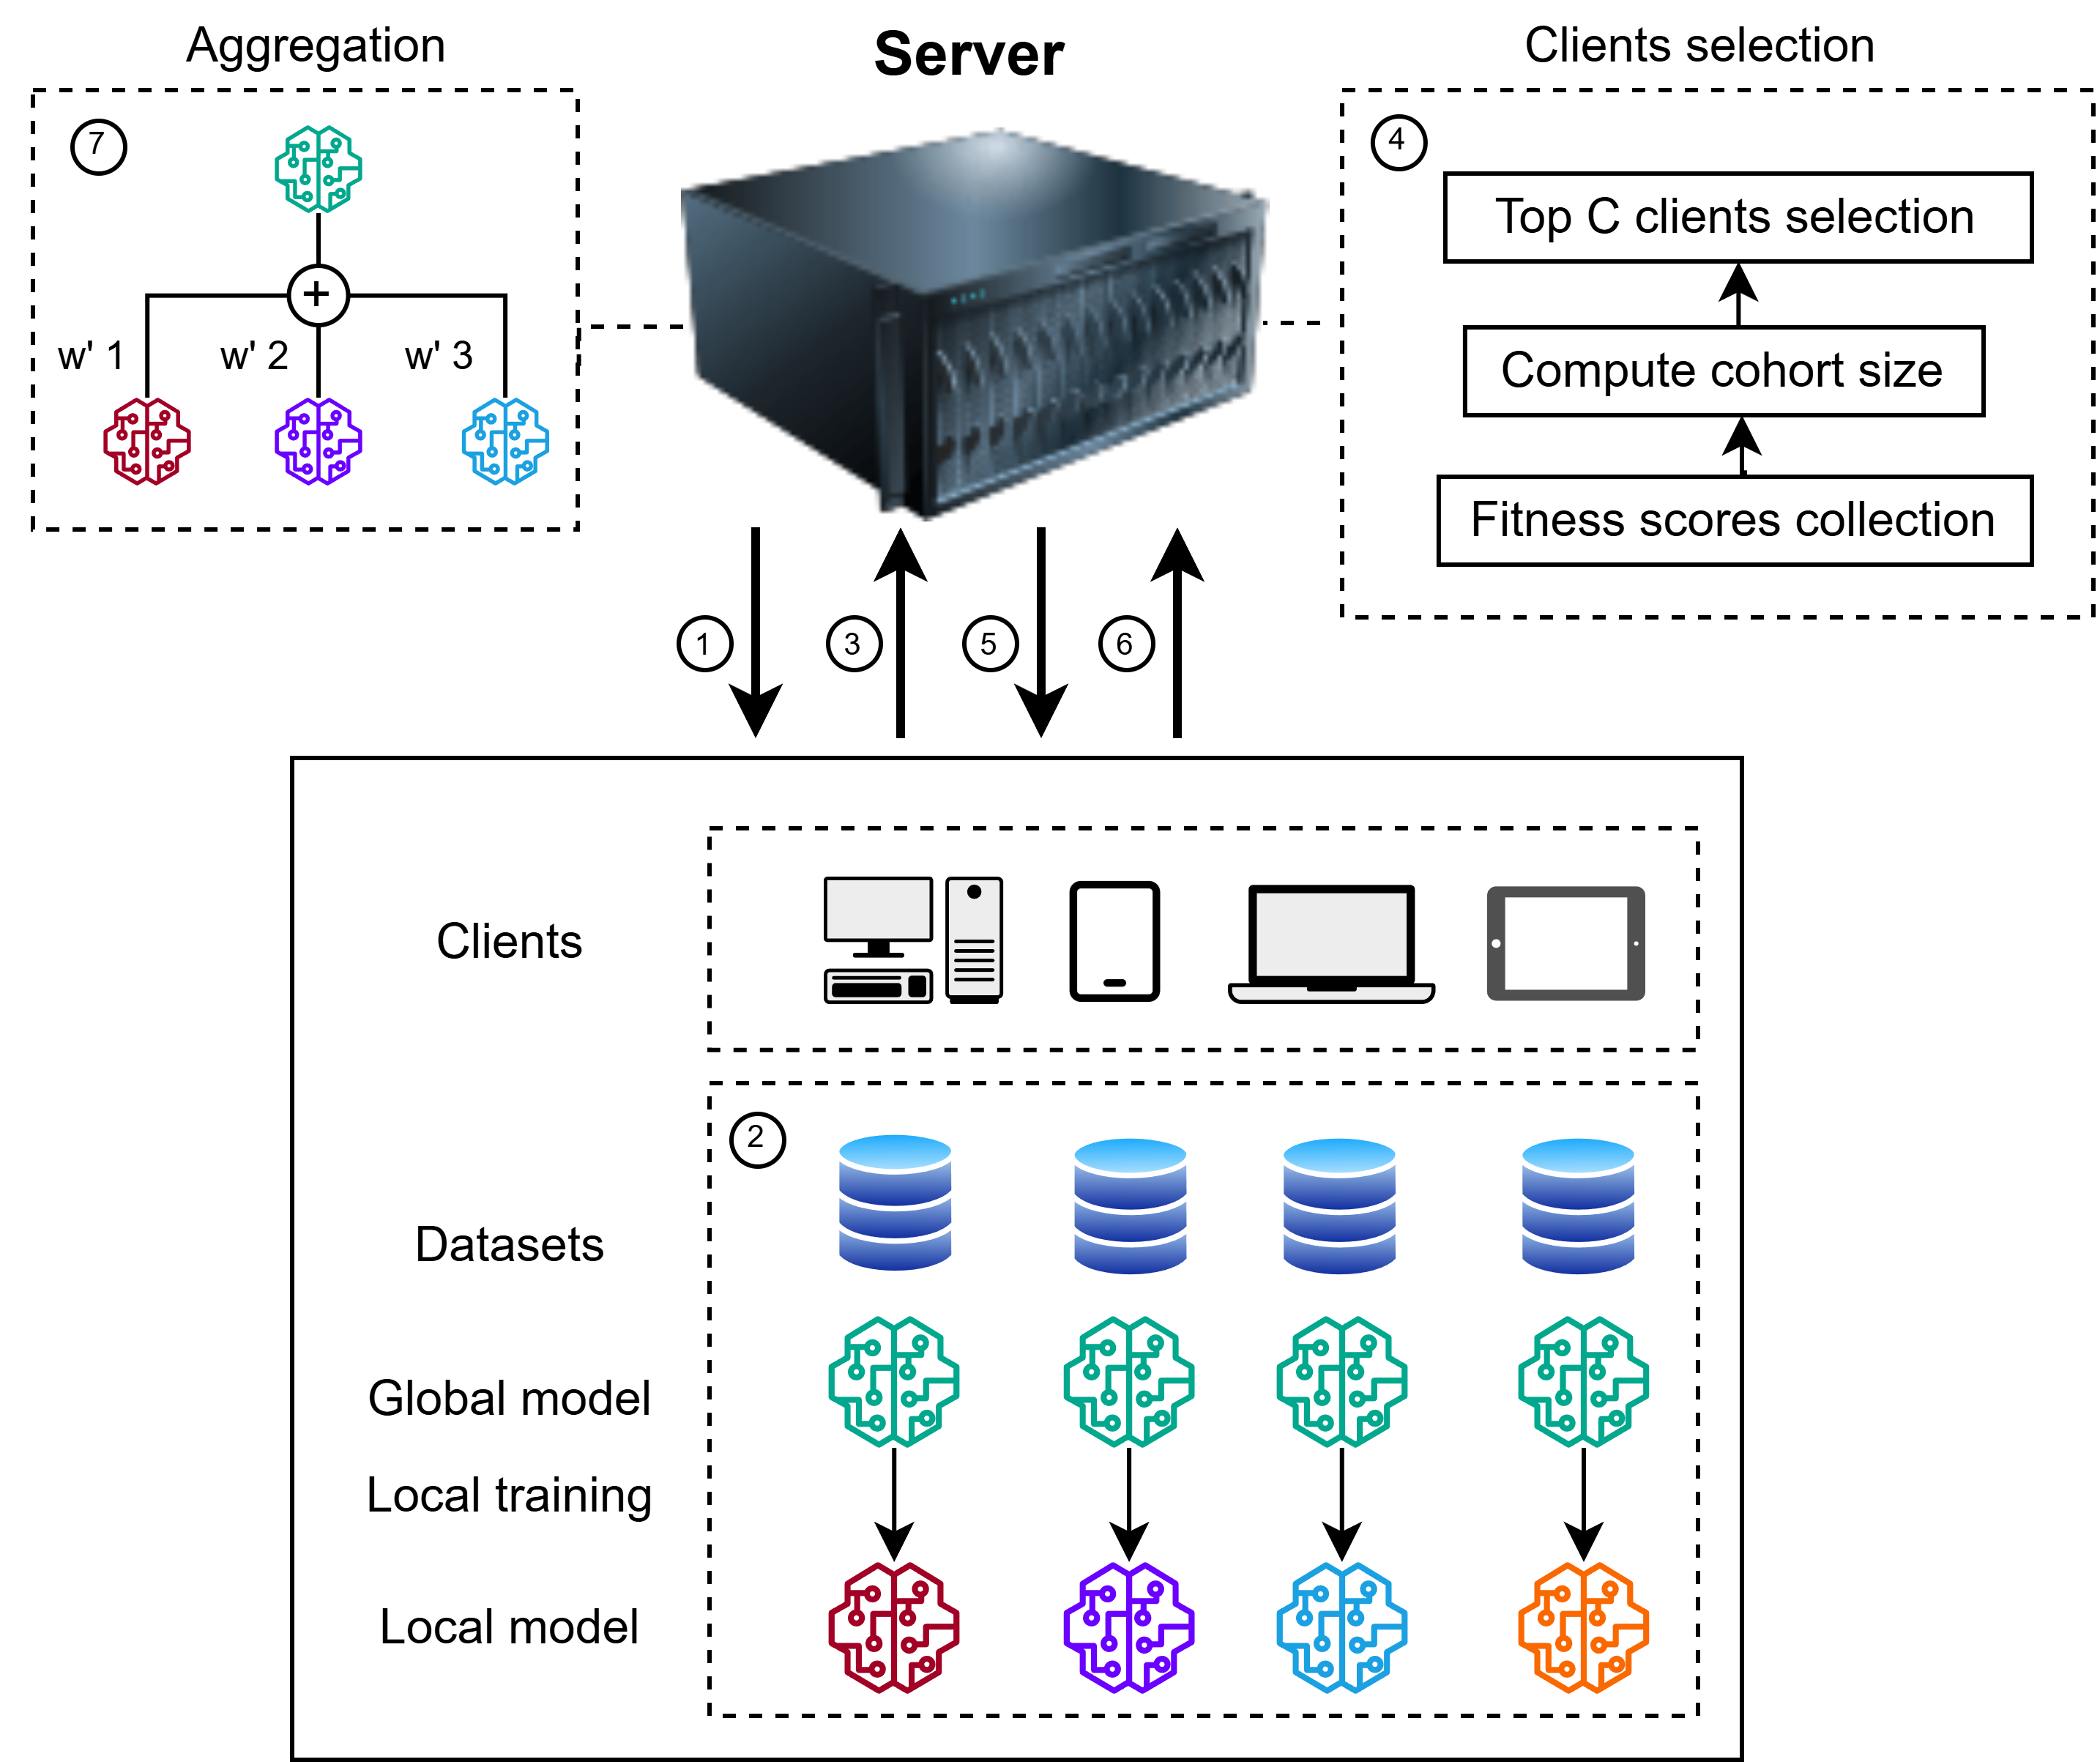
\includegraphics[width=0.7\textwidth]{figures/fig2.png}
\caption{Proposed framework architecture.}\label{fig:proposed_framework}
\end{figure}

The local training phase begins as the coordinating server delivers the current global parameters to participating clients for local model initialization, as shown in Fig. 2 (Step 1). During each training round, participating clients locally train the received global model and then computes its composite fitness selection score based on quantified balanced utility-fairness criteria and an uncertainty penalty (Step 2). Subsequently, each client transmits its composite score along with the number of consecutive idle rounds for evaluation (Step 3). Following this, clients are evaluated and ranked according to their composite fitness scores, and simultaneously cohort size is determined based on the global convergence efficiency to identify the top-ranked clients for participation in the subsequent iteration (Step 4). A subset of participating clients is selected by the server for contributing their updates to the aggregation process (Step 5). The selected clients submit their local updates for aggregation process (Step 6). 

Finally, the server adaptively weights the local models utilizing their stability scores before aggregation, producing the updated global model while updating the global fairness baseline for the next communication round (Step 7). Training proceeds iteratively until the model satisfies the required performance criteria or the specified limit on communication rounds is exhausted.

Algorithm 1 presents the client-side adaptive evaluation method in our proposed framework. The algorithm operates locally on each client to maximize and quantify their training effectiveness by computing a composite fitness score. At the beginning, the client receives the broadcasted global model for local training (Lines 3-8). It is then followed by computing an adaptive composite fitness score incorporating quantified KL divergence, fairness, and uncertainty penalty, while deriving the control parameter \textit{a} to balance utility and fairness according to the convergence state (Lines 12-18). To minimize communication overhead and preserve privacy, the client only transmits its composite fitness score to the server for ranking along with $r_i^t$ to calculate the global fairness baseline $r^t$ (Line 19). Finally, if the client is selected, it uploads its local model updates and stability score $s_i^t$ for aggregation (Lines 20-22).

\vspace{5mm}
    
%%---------- Algorithm 1 ----------%%
\begingroup
\small
\setlength{\tabcolsep}{3pt}
\renewcommand{\arraystretch}{0.92}

\noindent\textbf{Algorithm 1} Stability-Weighted Federated Aggregation
\par\noindent\rule{\linewidth}{0.4pt}
\vspace{1mm}

\noindent\textbf{Input:} $T$: communication rounds, $\{D_i\}$ local datasets of clients, $K$: total number of
clients, $Q(x)$, $P(x)$: predictions of global and local models respectively, $\eta$:
learning rate; $E$: local epochs, $w^t_{global}$: global model for round $t$, $\bar{r}^t$: Average idle
rounds across all clients, $v^{t+1}$: Deviation control signal, $C^t_k$: number of selected
clients $C \subset C$

\vspace{1mm}

\noindent\textbf{Output:} $w^t_i$: Local model update, $Fitness^t_i$: Fitness score, and $s^t_i$: Stability score.

\vspace{1mm}

\noindent\begin{tabular}{r@{\hspace{0.7em}}p{0.88\linewidth}}
1.  & \textbf{Initialize client model parameters} $w^t_i \leftarrow w^t_{global}$\\
2.  & \textbf{for every training round} $t = 1$ \textbf{to} $T$ \textbf{do}\\
3.  & \hspace{1em}\textbf{Receive global model parameters} $w^t_{global}$ \textbf{and control variables} $(\overline{r^t}, \nu^{t+1})$\\
4.  & \hspace{1em}\textbf{for every local epoch} $\in \{1, \ldots, E\}$ \textbf{do}\\
5.  & \hspace{2em}\textbf{for every batch of samples} $(x,y) \in D_c$ \textbf{do}\\
6.  & \hspace{3em}Compute forward pass of local model $\rightarrow P(x)$\\
7.  & \hspace{3em}Compute forward pass of global model $\rightarrow Q(x)$\\
8.  & \hspace{3em}Update the local model parameters: $w^t_i \leftarrow w^t_i - \eta \nabla L^t_{local}$\\
9.  & \hspace{2em}\textbf{end for}\\
10. & \hspace{1em}\textbf{end for}\\
11. & \hspace{1em}\textbf{After local training:}\\
12. & \hspace{2em}Compute $\Delta KL^t_i$ using (5)\\
13. & \hspace{2em}Compute $F^t_i$ using (6)\\
14. & \hspace{2em}Update control parameter $\alpha$ using (8)\\
15. & \hspace{2em}Compute priority $P^t_i$ using (9)\\
16. & \hspace{2em}Compute $\sigma^2_i$ using (12)\\
17. & \hspace{2em}Compute $s^t_i$ using (13)\\
18. & \hspace{2em}Compute $Fitness^t_i$ using (14)\\
19. & \hspace{2em}\textbf{Return} $Fitness^t_i$ and $r^t_i$ to server\\
20. & \hspace{1em}\textbf{If client} $i \in C^t_k$ //--(based on $Fitness^t_i$)\\
21. & \hspace{2em}\textbf{update} $r^{t+1}_i$\\
22. & \hspace{2em}\textbf{Return} $w^t_i, s^t_i$\\
23. & \hspace{1em}\textbf{Else update} $r^{t+1}_i$\\
24. & \hspace{1em}\textbf{End for}\\
\end{tabular}

\vspace{1mm}
\noindent\rule{\linewidth}{0.4pt}
\endgroup

\vspace{2mm}



%%---------- Algorithm 2 ----------%%
\begingroup
\small
\setlength{\tabcolsep}{3pt}
\renewcommand{\arraystretch}{0.92}

\noindent\textbf{Algorithm 2} Server-side Client Selection and Model Aggregation
\par\noindent\rule{\linewidth}{0.4pt}
\vspace{1mm}

\noindent\textbf{Input:} $T$: communication rounds, $\{D_i\}_{i=1,\ldots,N}$: local datasets of clients, $C$: total
number of clients, $\Omega^t$ reference convergence rate, $r^{t+1}_i$: number on idle consecutive
rounds, $w^t_i$: local model for client $i$, $Fitness^t_i$: fitness score, $s^t_i$: stability score.

\vspace{1mm}

\noindent\textbf{Output:} $w^{t+1}_{global}$: Global model, $\overline{r^{t+1}}$: Average fairness baseline, $\nu^{t+1}$: Deviation control signal.

\vspace{1mm}

\noindent\begin{tabular}{r@{\hspace{0.7em}}p{0.88\linewidth}}
1.  & \textbf{Initialize the global model parameters}\\
2.  & \textbf{For each communication round} $t \in \{1,\ldots,T\}$ \textbf{do}\\
3.  & \hspace{2em}Receive from clients: $\{Fitness^t_i\}$\\
4.  & \hspace{1em}\textbf{Sort} clients according to their fitness scores in descending order\\
5.  & \hspace{2em}Compute global convergence efficiency $(\rho)$ using (15)\\
6.  & \hspace{2em}Estimate number of top $C^t_k$ to select using (16)\\
7.  & \hspace{1em}\textbf{Select} $C^t_k$ clients with highest fitness scores\\
8.  & \hspace{1em}\textbf{Aggregate} selected clients' updates with stability weights:
$w^{t+1}_{global}=\displaystyle\sum_{i \in C_k} s^t_i \cdot w^t_i$\\
9.  & \hspace{1em}\textbf{Evaluate} updated global model on validation data\\
10. & \hspace{1em}\textbf{Update} $\overline{r^{t+1}}$ using (19)\\
11. & \hspace{2em}Compute $\nu^{t+1}$: $\nu^{t+1}=\Omega^{t+1}-\rho^{t+1}$\\
12. & \hspace{2em}Broadcast to all $C$ clients: $\{w^{t+1}_{global}, \nu^{t+1}, \overline{r^{t+1}}\}$\\
13. & \textbf{End for}\\
\end{tabular}

\vspace{1mm}
\noindent\rule{\linewidth}{0.4pt}
\endgroup



Furthermore, algorithm 2 outlines the overall procedure of server-side client selection and model aggregation. Clients are ranked according to their fitness scores. In addition, the cohort size is dynamically defined to select the top $C^t_k$ clients based on global convergence efficiency $\rho$ (Lines 3-7). The centralized server combines the locally trained models received from the selected clients using a stability-aware weighting strategy to construct an aggregated global model for the subsequent training (Lines 8).  Furthermore, the resulting global model is then validated using the validation dataset. (Lines 9). Every participating client is supplied with the latest global model, accompanied by the fairness baseline and the deviation control signal (Lines 10-13).


The proposed approach evaluates the effectiveness of each client using a composite fitness score that integrates three metrics reflecting utility, fairness, and uncertainty penalty under non-IID data conditions. The utility and fairness are adjusted based on global convergence efficiency to ensure the balance between exploitation and exploration in the system.

\subsection{FedFACS Methodology}
Each participating client is denoted by $C_i$, where $i \in \{1,\ldots,C\}$. At round $t$, the central server sends $w_{\text{global}}^t$ to all participating clients $C_i$. The KL divergence represents the client utility introduced previously in Eq. (3). Client $i$ produces the predictive distribution $P(x)$, where the corresponding global-model prediction is denoted by $Q(x)$, as defined in Eq. (5) (Amini et al. 2025). Furthermore, KL divergence is used as an indicator of the divergence between local and global predictive distributions, where larger values reflect a greater potential to improve the global model with new information. Therefore, selecting clients with higher KL divergence reduces the inconsistency between local and global predictive outputs, thereby enhancing model stability and generalization.
\begin{equation}
\Delta KL(P \parallel Q) = \sum_{x \in X} P(x)\log\left(\frac{P(x)}{Q(x)}\right)
\label{eq:kl}
\end{equation}

Fairness serves a vital function in preserving global model generalization. Without a fairness component, client selection approaches tend to repeatedly select a limited group of highly informative clients, leading to a biased global model toward particular data distributions while neglecting other less informative clients. The normalized fairness term in the proposed model is defined based on the consecutive idle rounds $r_i^t$ for client $i$, which is not selected up to round $t$. This is inspired by the Age Of Information (AOI) metric (Xu et al., 2024), and the average idle rounds across all participating clients at communication round $t$, represented by $\overline{r^t}$, which the server computes, as shown in Eq.~(6). The normalization is scale-invariant and prevents division by zero during the initial training round or when all clients are selected by the server, while adding 1 to the fraction as a baseline offset to ensure numerical stability. In addition, it evaluates a client’s need for participation relative to the current client activity.
\begin{equation}
F_i^t = 1 + \frac{r_i^t}{1 + \overline{r^t}}
\label{eq:fairness}
\end{equation}

The counter of idle rounds $r_i^t$ is updated every round according to Eq.~(7), where $C_k^t$ denotes the size of the client cohort selected at round $t$.

\begin{equation}
r_i^{t+1} =
\begin{cases}
0 & \text{if } i \in C_k^t  \\
r_i^t & \text{otherwise}
\end{cases}
\label{eq:idle_update}
\end{equation}

The proposed control mechanism is inspired by the Lyapunov stability principle, where the feedback signal guides the system in determining whether to shift toward informativeness or fairness. At the same time, the use of bounded and normalized updates helps ensure stable behavior during training. The control mechanism is defined as follows:
\begin{equation}
a_i^t = clip(a,1,0) = \prod_{[0,1]}
\left(
\beta \cdot a_i^{t-1} + (1-\beta)
\frac{
\nu^t \cdot (\Delta KL_i^t - F_i^t)
}{
\lambda \cdot F + \nu^t \cdot (\Delta KL_i^t - F_i^t)
}
\right)
\end{equation}


The term $\Delta KL_i^t - F_i^t$ provides a directional signal for decision-making, while incorporating the fairness term in the denominator helps stabilize the update and avoids rapid shifts caused by under-served clients. This leads to a smooth and balanced control mechanism. The parameter $\beta \in [0,1]$ is an exponential moving average smoothing parameter, $\lambda$ is a fairness regularization coefficient, and $\prod_{[0,1]}(\cdot)$ represents the Euclidean projection to ensure that the parameter remains within the bounded interval.

The fairness value increases when a client remains unselected, forcing other metrics in the priority score to encourage its selection as in Eq. (9), where the contribution of client $i$ during communication round $t$ is represented by the priority score $p_i^t$. This score combines two main factors such as: fairness and utility while weighting them through a control mechanism by tuning the control parameter $a$, allowing the framework to prioritize fairness or utility depending on the global model’s needs for either exploitation or exploration.
\begin{equation}
P_i^t = a \cdot \Delta KL_i^t + (1 - a)\, F_i^t
\label{eq:priority}
\end{equation}

By adjusting the control parameter $a_i^t \in [0,1]$, the control mechanism dynamically balances informativeness against fairness. This parameter is updated based on the feedback deviation control signal $\nu^t$, which reflects the current convergence behavior of the global model.

The deviation control signal $\nu^t$ is computed on the server side and defined as the difference between the adaptive reference convergence rate $\Omega^t$ and the current global convergence efficiency $\rho^t$, as shown in Eq.~(10). This signal acts as the main feedback mechanism that adaptively adjusts the exploration--exploitation balance at each training round.
When $\nu^t > 0$, the convergence is slower than the reference rate, leading to an increase in the control parameter $a_i^t$ to prioritize the selection of informative clients and accelerate convergence. Conversely, when $\nu^t \le 0$, the convergence is faster than the reference rate, leading to a decrease in the control parameter to prioritize fairness and improve client participation.
Therefore, the introduction of the deviation control signal is essential for providing the framework with performance-aware behavior.
\begin{equation}
\nu^t = \Omega^t - \rho^t
\label{eq:deviation}
\end{equation}

\begin{equation}
\Omega^t = \gamma^t \cdot \rho_{\text{base}}^t
\label{eq:reference_rate}
\end{equation}

Equation (11) defines the adaptive reference convergence rate $\Omega^t$, which guides the control signal to balance exploitation and exploration. Here, $\rho_{\text{base}}^t$ represents the convergence rate obtained from a prior run of a standard baseline model or state-of-the-art algorithm under identical experimental conditions, and $\gamma$ denotes an acceleration index.

Client-side uncertainty is introduced into the fitness score as a variance based penalty term. It quantifies KL estimate across several small batches of local client’s dataset. This term penalizes the clients whose data is highly unstable or non-representative data (i.e., high variance), even having a high utility as its variability between samples indicates that the data might be noisy or contain extreme outliers. While the clients with low uncertainty score reflect their stability that enhances robustness and stability under heterogeneous scenarios. The uncertainty penalty term for client \textit{i} is defined as:

\begin{equation}
\sigma_i^2 = \frac{1}{B-1} \sum_{b=1}^{B} \left( KL_i^b - \overline{KL}_i \right)^2
\label{eq:variance}
\end{equation}

Where $B$ indicates the total count of mini batches, $\overline{KL_i}$ represents the average KL-divergence over batches for client $i$, and $KL_i^b$ is the KL-divergence of batch $b$.

The stability score is derived from Eqs. (5) and (12). This score is used for weighting the local model updates in aggregation step. It prioritizes the informative and stable clients over less informative ones to stabilize and accelerate the convergence in heterogeneous data environments without affecting fairness. The formula of stability score is defined as follows:

\begin{equation}
s_i^t = \Delta KL_i^t - \mu \sigma_i^2
\label{eq:stability}
\end{equation}

The following equation summarizes the calculation formula of the composite fitness score: 
\begin{equation}
Fitness_i^t = P_i^t - \mu \sigma_i^2
\label{eq:fitness}
\end{equation}

Where $\mu$ is a regularization coefficient. Finally, each client sends its fitness score ${Fitness}_i^t$ along with the number of consecutive idle rounds $r_i^t$ to the server for evaluation. When the client is selected $i\in C_k^t$, it uploads its local model updates $w_i^t$  for aggregation and updates its idle rounds counter to $r_i^{(t+1)}$.

On the server-side, it receives fitness scores from all clients for evaluation. The server ranks the clients according to their fitness scores and adaptively determines the cohort size according to the convergence efficiency observed in the previous communication round, which represents the reduction rate of the global loss value $\rho \in  [0, 1]$ as shown in Eq. (15). Two predefined bounds, $C_{k_{\min}}$ and $C_{k_{\max}}$, regulate the allowable cohort size range (McMahan et al. 2017; Li et al. 2020), thereby enabling an adaptive number
of clients to be selected for aggregation while maintaining communication efficiency and mitigating network congestion, as defined in Eq. (16).
\begin{equation}
\rho^{t-1} = \frac{L_{{global}}^{t-2} - L_{{global}}^{t-1}}{L_{{global}}^{t-2}}
\label{eq:convergence}
\end{equation}

\begin{equation}
C_k^t = C_{k_{\min}} + \left( (C_{k_{\max}} - C_{k_{\min}})\cdot (1 - \rho^{t-1}) \right)
\label{eq:ck_selection}
\end{equation}

When $\rho$ indicates sharp improvement, the cohort size is dynamically decreased reducing communication overhead. In contrast, during stagnation and degradation, the cohort size increases, requesting updates from more informative clients to improve global model accuracy and push it out of a local optimum.

Once the selected clients submit their local updates, normalization is applied to preserve the exact proportional differences in client quality, as shown in Eq. (18), where \textit{S} represents the normalized sum. Following this, the server carries out a stability-weighted aggregation, which is formulated as follows:

\begin{equation}
w_{{global}}^{t+1} = \sum_{i \in C_k^t} S_i^t \, w_i^t
\label{eq:stability_weighted_update}
\end{equation}

\begin{equation}
S_i^t = \frac{s_i^t}{\sum_{i \in C_k^t} s_i^t}
\label{eq:stability_norm}
\end{equation}

One more step, the resulting model is assessed on a separate validation set, then the centralized server updates its deviation control signal and global fairness baseline as defined in Eq.~(19). As the final step, the resulting global model parameters $w_{{global}}^{t+1}$, $\overline{r^{t+1}}$, and $\nu^{t+1}$ are broadcast to the entire set of $C$ clients for the following training round.

\begin{equation}
\overline{r^{t+1}} = \frac{1}{K} \sum_{i=1}^{K} r_i^t
\label{eq:avg_idle_correct}
\end{equation}

The proposed approach introduces a fitness scoring method that ensures the selection of high-quality and and informative clients, while preserving fair participation according to client’s informativeness and the current level of model convergence. This allows the framework to explore clients that may provide useful information during stable improvement, allowing them to contribute. However, it forces the system to exploit the more informative clients during degradation, preventing bias in the global model and preserving balance when system stagnates. As a result, the proposed approach enhances the overall performance by improving accuracy, reducing communication overhead by selecting the more contributing clients to send their updates, and ensuring fair participation. 

Furthermore, the aggregation process incorporates stability-based weighting, reflecting the effectiveness and relative contribution across individual client models with respect to its stability score. This approach assigns higher aggregation weights to the informative and stable clients. In addition, it does not compromise fairness but only reduces the implications arising from exploring less utility clients, while assigning lower weights to less informative clients.

\section{Experimental Evaluation}\label{sec5}

\subsection{Datasets}

For performance evaluation of the proposed framework, extensive experimental evaluations were carried out using four widely used benchmark multimedia datasets. These datasets include MNIST, FMNIST, CIFAR-10, and the COVID-19 Radiography dataset. MNIST and FMNIST contain 60,000 training images and 10,000 test images, with each sample represented as a 28 \ensuremath{\times} 28 grayscale image. MNIST covers handwritten digit recognition, while FMNIST consists of images from ten clothing-related categories. In addition, CIFAR-10 extends the evaluation to natural RGB images, comprising 60,000 samples of size 32 \ensuremath{\times} 32 pixels organized into ten categories (Krizhevsky and Hinton 2009). To extend the evaluation, the COVID-19 radiography database was used to assess the framework under a real-world medical imaging scenario. It comprises chest radiographs from three classes: COVID-19, normal, and viral pneumonia (Rahman et al. 2020).  

To assess the proposed framework under heterogeneous data conditions, the training data are partitioned using four distinct scenarios to model varying degrees data heterogeneity across clients. In the first scenario (S1), a Dirichlet distribution $\mathrm{\textit{Dir}}(\alpha)$ is applied to distribute training samples among clients with the distribution parameter $\alpha \in \{0.1, 0.5\}$ to generate imbalanced datasets in both size and label distribution, where a smaller value of $\alpha$ leads to higher data skewness (Iyer. 2023). In the second scenario (S2), clients are randomly assigned data from two classes (Zhai et al. 2024). In the third scenario (S3), a number of noisy data is generated and distributed across the clients with a noise level ranging from 0\% to 45\% per client under IID conditions. In the fourth scenario (S4), three clients contain data from all ten classes with noise levels of 10\% and 20\%, while the remaining clients contain data from only nine classes with the noise patterns described in S3, under non-IID conditions (Shi et al. 2023).

\subsection{Model and experimental setup}

\textbf{Benchmark.} The comparisons are made across established federated learning baselines and recent adaptive selection methods. The proposed FedFACS framework is compared against several approaches, such as FedAvg (McMahan et al. 2017), FedProx (Li et al. 2020), DivFL (Balakrishnan et al. 2022), Power-of-Choice (Cho et al. 2022), and the approach introduced by Zhai et al. (2024) to evaluate performance and communication efficiency. 

Furthermore, FedFACS is compared against a Random baseline that selects clients randomly in each communication round, Power-of-Choice, and AHIBCS (Liu et al. 2025), a recent adaptive selection method. This comparison specifically evaluates the accuracy and convergence speed of FedFACS against the most closely related existing selection strategy, thereby validating the robustness of the presented framework.

In addition, for evaluating the balance between fairness and performance, the proposed approach is compared against four client selection strategies: a Random baseline, a Greedy strategy that prioritizes clients with the highest reputation, the RBFF method proposed by Song et al. (2022), and the FedFairCS approach introduced by Shi et al. (2023).

\textbf{Model}. The proposed FedFACS approach was implemented in Python using PyTorch and Torch-vision, employing a fine-tuned ResNet-18 (He et al. 2021) to achieve stable training. This architecture delivers high accuracy with low computational complexity, where the early blocks including the convolutional layer 1 and layers 1-3 are frozen, while the layer 4 and the final fully connected layer are trained and adjusted for 10 classes.

\textbf{Hyperparameters}. The experimental evaluation is conducted under three distinct configurations, each is designed to test the proposed model under different conditions. For configuration A, all the methods follow the same hyperparameter settings as in (Zhai et al. 2024). The federated learning environment is simulated with a single centralized server and 100 decentralized clients. The experiments are carried out for 200 training rounds, under a local training setup consisting of 10 epochs, a batch size of 32, $\beta = 0.9$, and the maximum client sampling rate $C_{k\max}$= 0.1. The models were trained via Stochastic Gradient Descent (SGD), with learning rates of 0.05 and 0.01 are adopted for CIFAR-10 and both FMNIST and MNIST, respectively. The proximal coefficient in FedProx is set to 0.1. For the Power-of-Choice (Pow-D), 10 highest-loss clients are selected out of a randomly sampled set of 20. These experiments are to compare the proposed model against FedAvg, FedProx, Power-of-Choice, and the approach of (Zhai et al. 2024), highlighting the performance and communication efficiency under data distributions described in scenarios 1 and 2.

Configuration B follows the experimental setup proposed in (Liu et al. 2025). Additional experiments were carried out using the FMNIST, CIFAR-10, and COVID-19 benchmark datasets. Model training was performed over 100 communication rounds on FMNIST and 350 rounds on both CIFAR-10 and COVID-19, with the learning rates of 0.001, 0.1, and 0.01, respectively. The FMNIST and CIFAR-10 experiments were performed with 100 participating clients, whereas the COVID-19 experiments were conducted using 30 participating clients. For the competing methods Random, Pow-D, and AHIBCS, at every training iteration, a total of 15 clients were chosen at random, from which 10 clients were selected for model aggregation.

For configuration C, additional experiments are conducted with learning rates configured to 0.005 for CIFAR-10 and 0.01 for FMNIST, respectively. Training continues until no further improvement in the global loss is observed over 20 consecutive communication rounds. A batch size of 64 is adopted with 20 local training epochs. In FedFairCS, the control parameter $\sigma$ is fixed at 0.6. This experiments evaluates the proposed model against Random, Greedy, RBFF, and FedFairCS, focusing on fairness-accuracy balance under data distributions described in scenarios 3 and 4.

\textbf{Performance metrics}. The proposed framework is examined with respect to performance, fairness, and communication efficiency using the following evaluation metrics:

\textit{Accuracy}: refers to the rate of correct classifications produced by the trained model over the test samples.

\textit{Round-to-accuracy}: defines the training iteration count required to reach a specified accuracy. This metric provides an assessment of the convergence efficiency of the client selection strategy and the communication cost associated with achieving the desired performance, where fewer communication rounds indicate faster convergence and lower communication requirements.

\textit{Recall and F1 score}: Recall reflects the true positive rate, while the F1 score provides a comprehensive and balanced assessment of classification capability by incorporating precision and recall (Yacouby and Axman 2020; Liu et al. 2025). 
\begin{equation}
\text{Recall} = \frac{TP}{TP + FN}
\label{eq:recall}
\end{equation}

\begin{equation}
\text{Precision} = \frac{TP}{TP + FP}
\label{eq:precision}
\end{equation}

\begin{equation}
F1 = 2 \times \frac{\text{Precision} \times \text{Recall}}
{\text{Precision} + \text{Recall}}
\label{eq:f1_score}
\end{equation}



In the formulation, $TP$, $FP$, and $FN$ indicate correctly detected, incorrectly predicted, and missed positive instances, respectively. These metrics evaluate the performance, stability, and generalization ability of FedFACS under non-IID conditions.


\textit{Cumulative number of selected clients until convergence  ($C_{total}$)}: indicates the overall number of clients selected for aggregation across all training rounds before the global model reaches the target accuracy.

\begin{equation}
C_{\text{total}} = \sum_{t=1}^{T} C_k^t
\label{eq:communication}
\end{equation}

\textit{Jain’s Fairness Index (JFI)}: quantifies client-selection fairness using the number of times each client is selected throughout training (Shi et al. 2024; Cho et al. 2020).
\begin{equation}
JFI = \frac{\left(\sum_{i=1}^{n} \frac{p_i}{q_i}\right)^2}
{n \cdot \sum_{i=1}^{n} \left(\frac{p_i}{q_i}\right)^2}
\label{eq:jfi}
\end{equation}

\begin{equation}
q_i = (\text{number of labels}) \times (1 - \text{percentage of noisy data})
\label{eq:qi}
\end{equation}

For client $i$, $p_i$ reflects its rate of participation in model aggregation, while $n$ denotes the overall client population, and $q_i$ represents the quality of its locally stored dataset (Shi et al. 2023). When $JFI = 1$, it refers to equal participation for all clients, when the values in the range $0.5 \leq JFI < 1$ indicate that all clients participates with different times, and values below $0.5$ represent the unfair participation.

\subsection{Experimental Results and Analysis}

The evaluation of FedFACS was conducted across a range of heterogeneous data distribution conditions, with the experiments performed on a system using an Nvidia RTX 3090 GPU and 32 GB of RAM.

The relative contribution of each component in FedFACS is individually evaluated through a comprehensive ablation study. The components are the full FedFACS, FedFACS-A1 which removes both of adaptive aggregation and cohort sizing (Ablation 1), where client selection is performed with a constant sampling size of ($C_k^t=10$) and static weighted aggregation is used (McMahan et al. 2017), and FedFACS-A2 that utilizing dynamic cohort sizing with ($C_{k_{\min}} = 8$) and ($C_{k_{\max}} = 10$) removes adaptive aggregation only (Ablation 2). The experimental setup follows configuration A, and The target accuracy is determined as the maximum accuracy obtained by FedAvg under the corresponding experiments with data partitioning conditions presented in scenarios 1 and 2.

Tables 1 and 2 demonstrate the improvements achieved by FedFACS-A1 that incorporates the proposed adaptive client selection mechanism, including higher predictive accuracy while reducing the communication rounds required to attain the target accuracy. Moreover, introducing dynamic cohort sizing in FedFACS-A2 leads to a slight change in accuracy due to the adaptive reduction in participating clients, and reduces communication overhead by selecting approximately 15\% fewer clients per training round. Furthermore, incorporating the adaptive stability-weighted aggregation in the full FedFACS model limits the effect of gradient noise from unstable clients by assigning larger aggregation weights to stable and informative client updates. Consequently, the aggregated global model becomes more robust, mitigating the impact of noisy clients and accelerating convergence with fewer training rounds.

\FloatBarrier

\FloatBarrier

%% Tables 1 and 2 %%
\begin{table}[!htbp]
\centering
\footnotesize
\setlength{\tabcolsep}{4pt}
\renewcommand{\arraystretch}{1.08}
\setlength{\abovecaptionskip}{2pt}
\setlength{\belowcaptionskip}{3pt}

\caption{Accuracy comparison of FedFACS and its ablated variants under different data heterogeneity conditions.}
\label{tab:ablation_accuracy}

\begin{tabular*}{\journalfloatwidth}{@{\extracolsep{\fill}}llccc@{}}
\toprule
Dataset & Scenario & FedFACS-A1 & FedFACS-A2 & FedFACS \\
\cmidrule(lr){3-5}
 &  & Acc. (\%) & Acc. (\%) & Acc. (\%) \\
\midrule
CIFAR-10 & S1 ($\alpha=0.1$) & 46.89 & 46.70 & \textbf{47.07} \\
         & S1 ($\alpha=0.5$) & 50.37 & 49.95 & \textbf{51.12} \\
         & S2                 & 46.92 & 46.61 & \textbf{47.33} \\

MNIST    & S1 ($\alpha=0.1$) & 98.23 & 98.12 & \textbf{98.52} \\
         & S1 ($\alpha=0.5$) & 98.63 & 98.48 & \textbf{98.91} \\
         & S2                 & 97.75 & 97.61 & \textbf{98.11} \\

FMNIST   & S1 ($\alpha=0.1$) & 86.35 & 86.19 & \textbf{86.63} \\
         & S1 ($\alpha=0.5$) & 88.35 & 87.91 & \textbf{88.95} \\
         & S2                 & \textbf{83.81} & 83.76 & 83.80 \\
\bottomrule
\end{tabular*}

\vspace{15pt}

\caption{Communication rounds required by FedFACS and its ablated versions to achieve the target accuracy under different data heterogeneity conditions.}
\label{tab:round_to_accuracy_ablation}

\begin{tabular*}{\journalfloatwidth}{@{\extracolsep{\fill}}llccc@{}}
\toprule
Dataset & Scenario & FedFACS-A1 & FedFACS-A2 & FedFACS \\
\cmidrule(lr){3-5}
 &  & Round & Round & Round \\
\midrule
CIFAR-10 & S1 ($\alpha=0.1$) & 47 & 44 & \textbf{40} \\
         & S1 ($\alpha=0.5$) & 69 & 64 & \textbf{57} \\
         & S2                 & 117 & 115 & \textbf{110} \\

MNIST    & S1 ($\alpha=0.1$) & 67 & 62 & \textbf{58} \\
         & S1 ($\alpha=0.5$) & 72 & 73 & \textbf{69} \\
         & S2                 & 123 & 117 & \textbf{115} \\

FMNIST   & S1 ($\alpha=0.1$) & 85 & 83 & \textbf{81} \\
         & S1 ($\alpha=0.5$) & \textbf{97} & 103 & 99 \\
         & S2                 & 111 & 113 & \textbf{105} \\
\bottomrule
\end{tabular*}

\end{table}

\FloatBarrier


\begin{figure}[!htbp]
\noindent
\begin{minipage}{\linewidth}
\centering

\begin{minipage}[t]{0.32\linewidth}
    \centering
    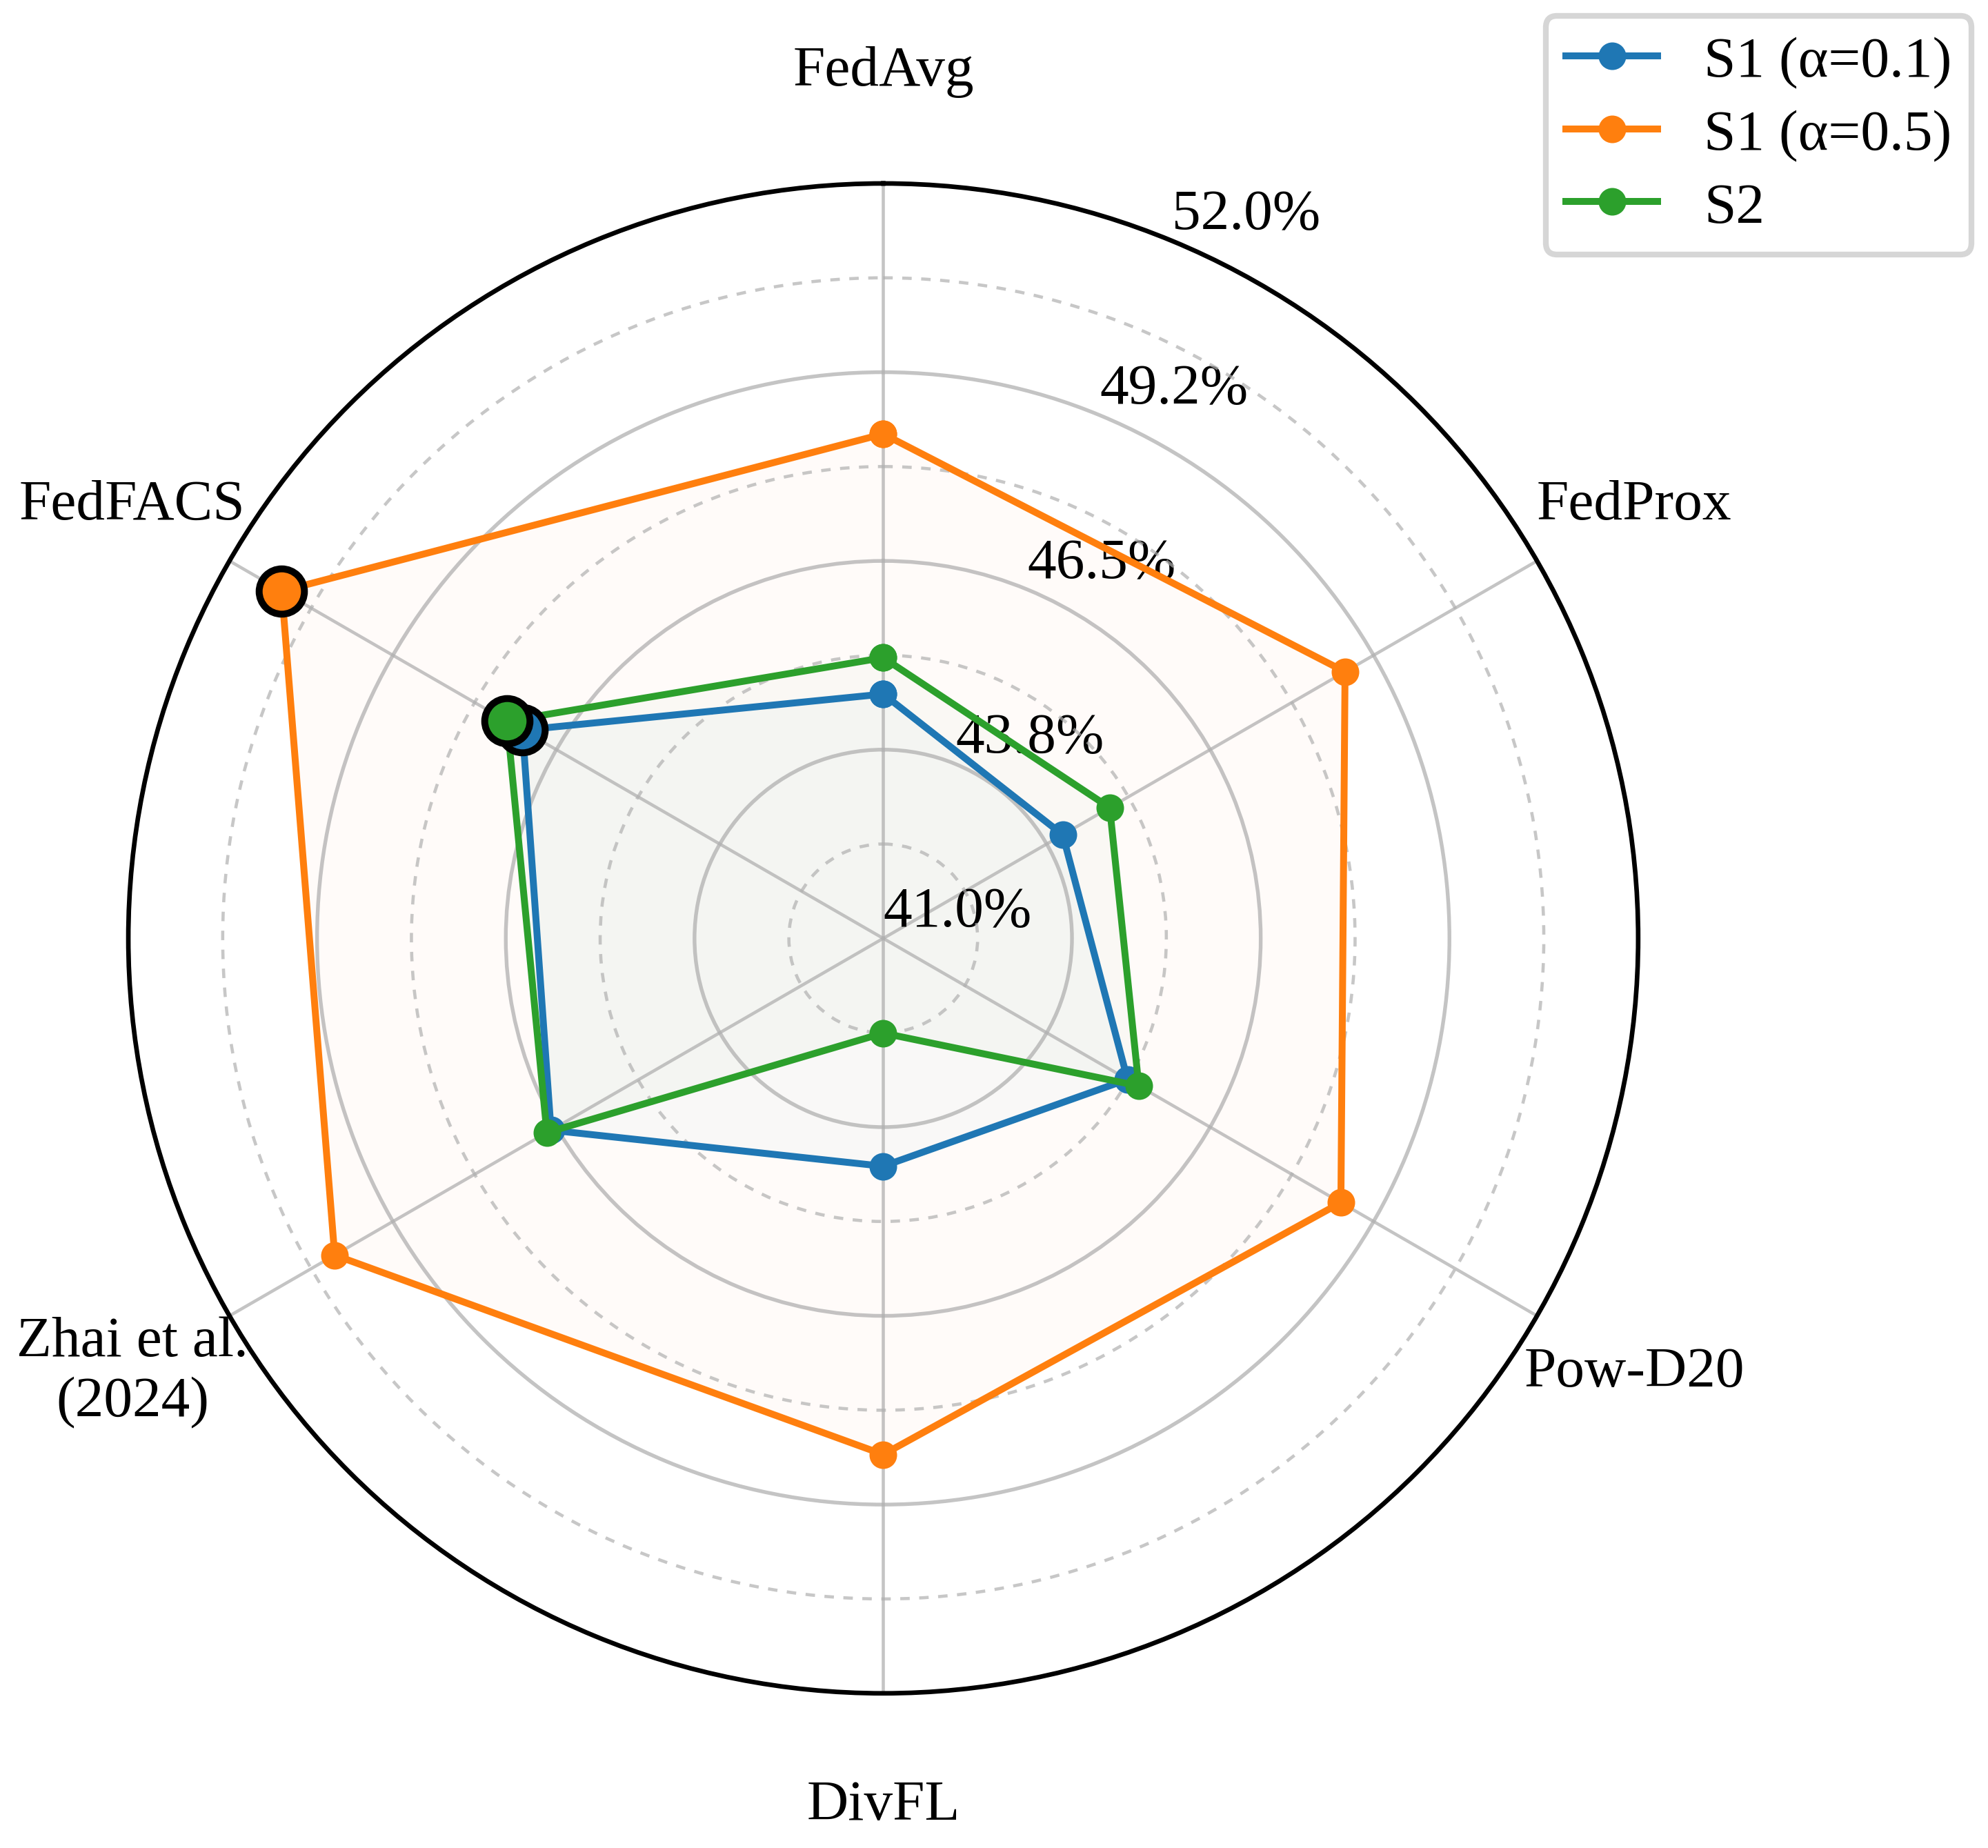
\includegraphics[
        width=\linewidth,
        height=0.3\textheight,
        keepaspectratio
    ]{figures/fig3_a_radar_cifar.png}
    \vspace{1mm}
    {\footnotesize (a) CIFAR-10}
\end{minipage}
\hfill
\begin{minipage}[t]{0.32\linewidth}
    \centering
    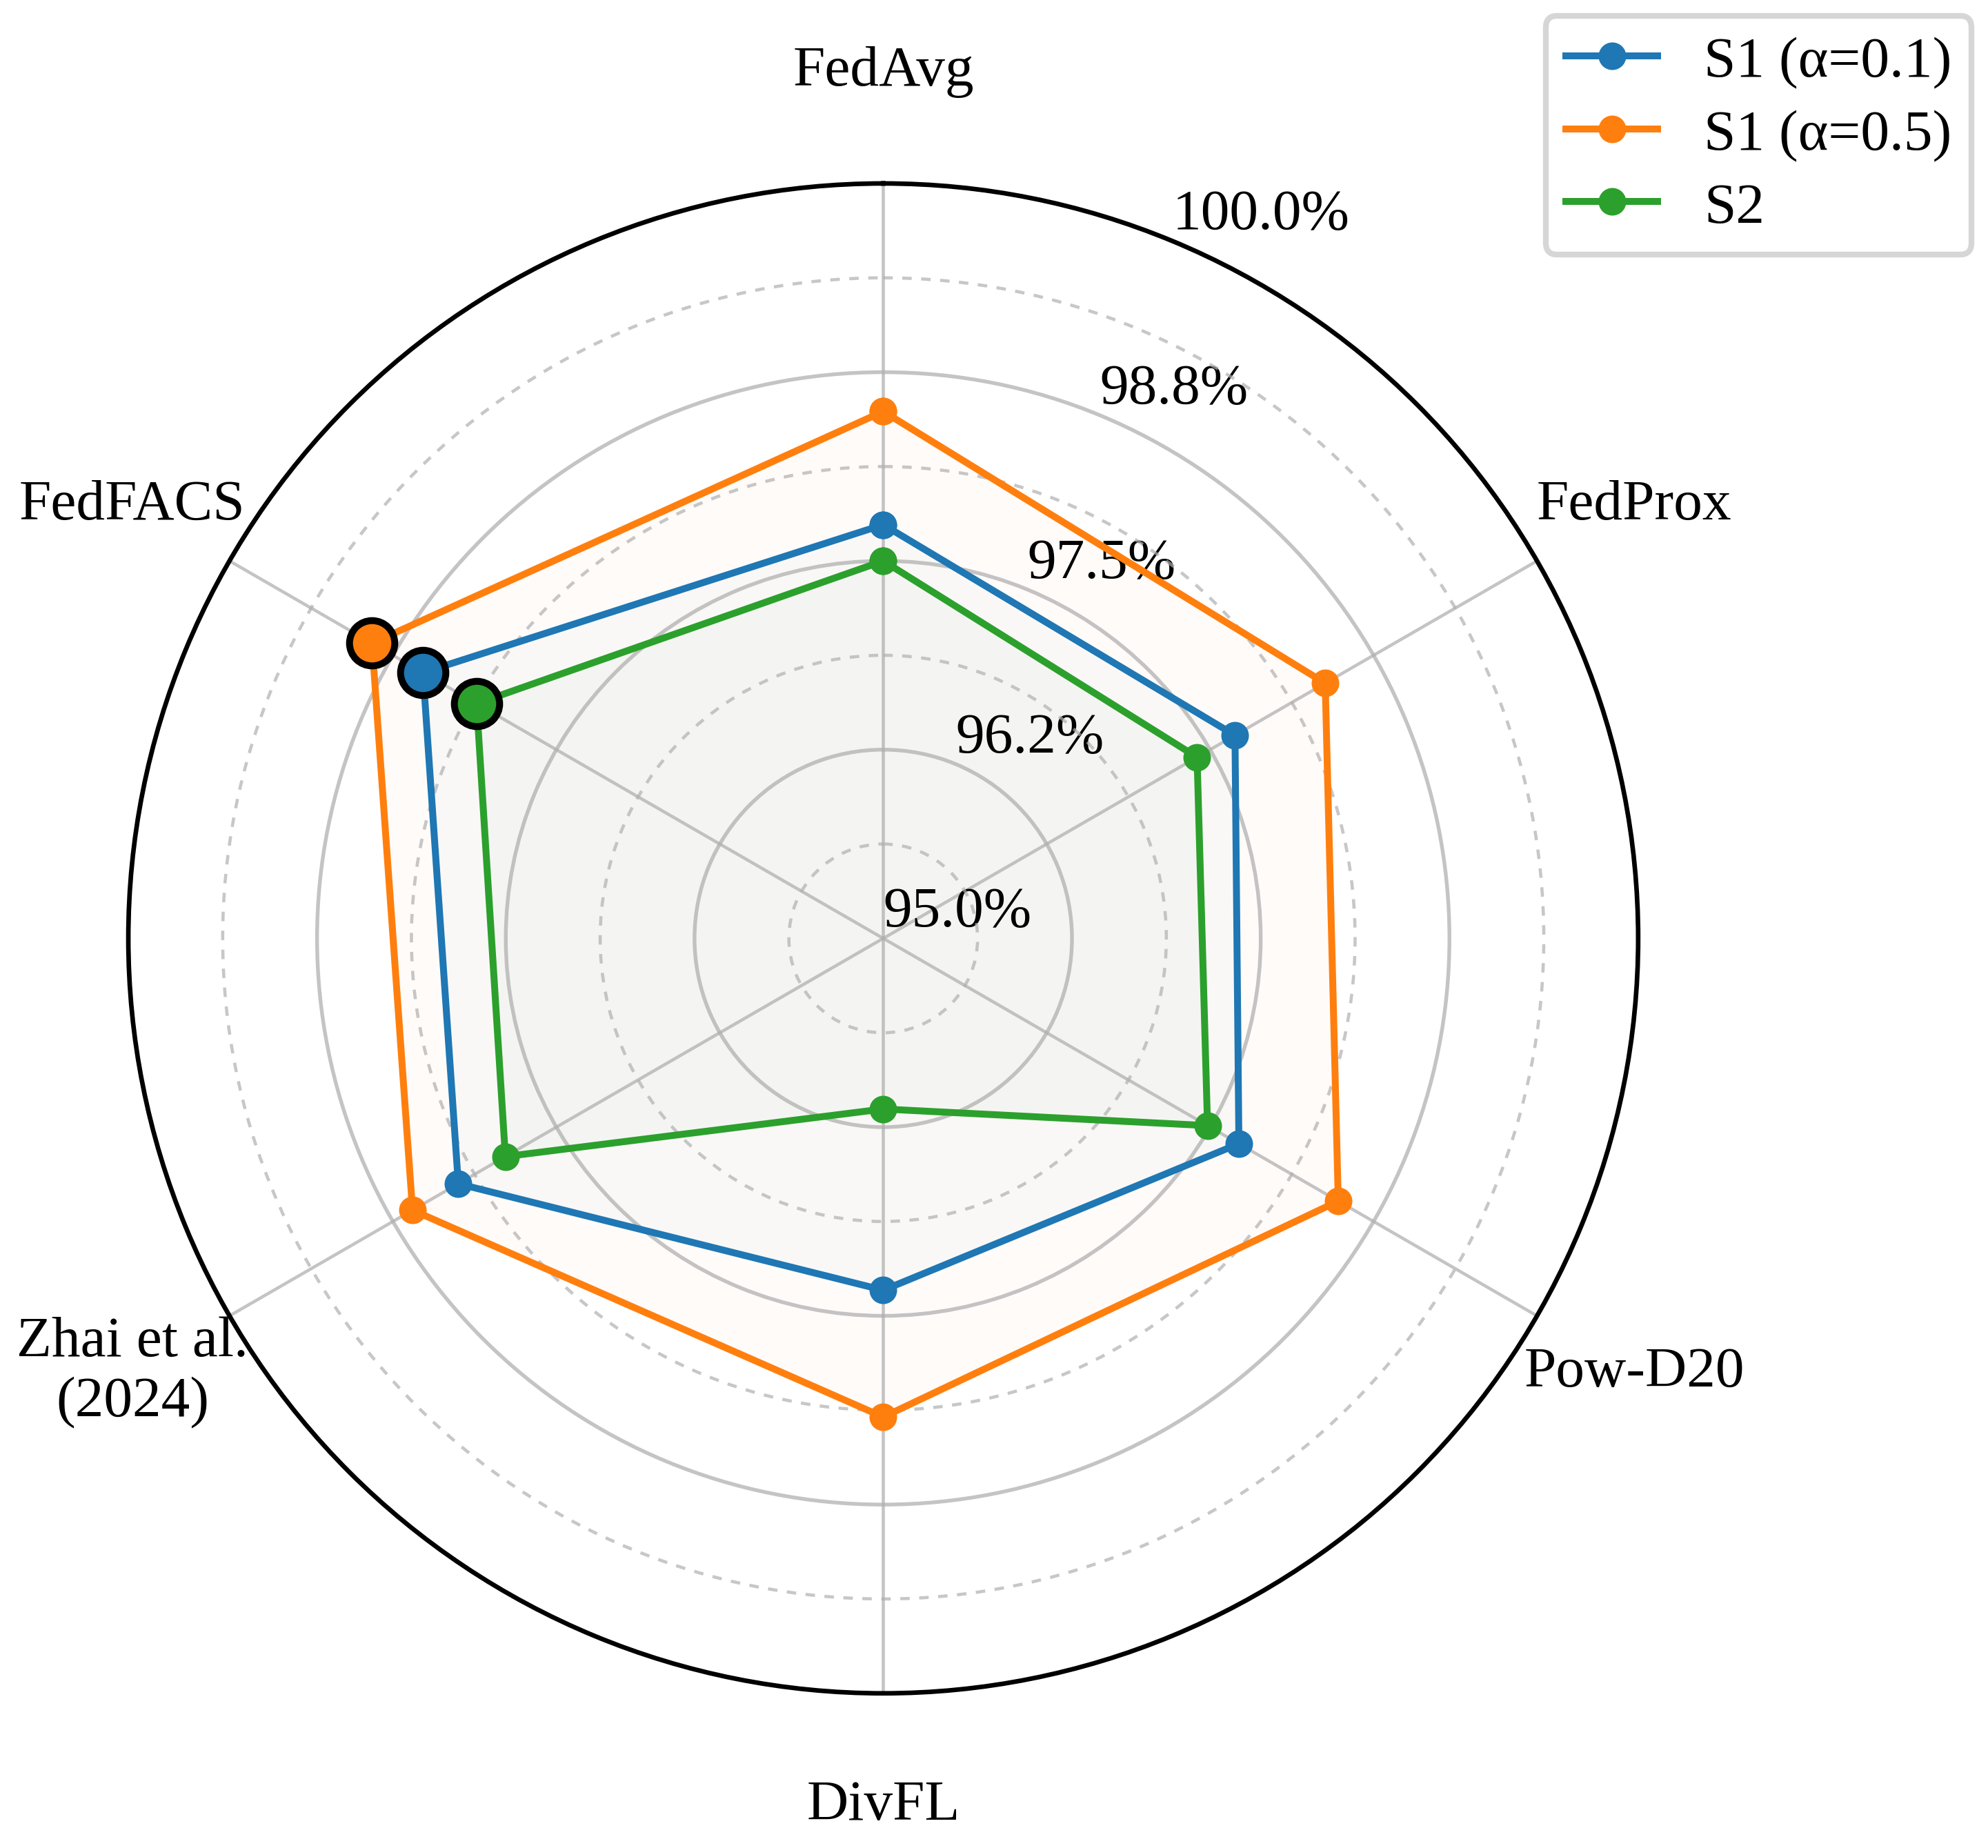
\includegraphics[
        width=\linewidth,
        height=0.3\textheight,
        keepaspectratio
    ]{figures/fig3_b_radar_mnist.png}
    \vspace{1mm}
    {\footnotesize (b) MNIST}
\end{minipage}
\hfill
\begin{minipage}[t]{0.32\linewidth}
    \centering
    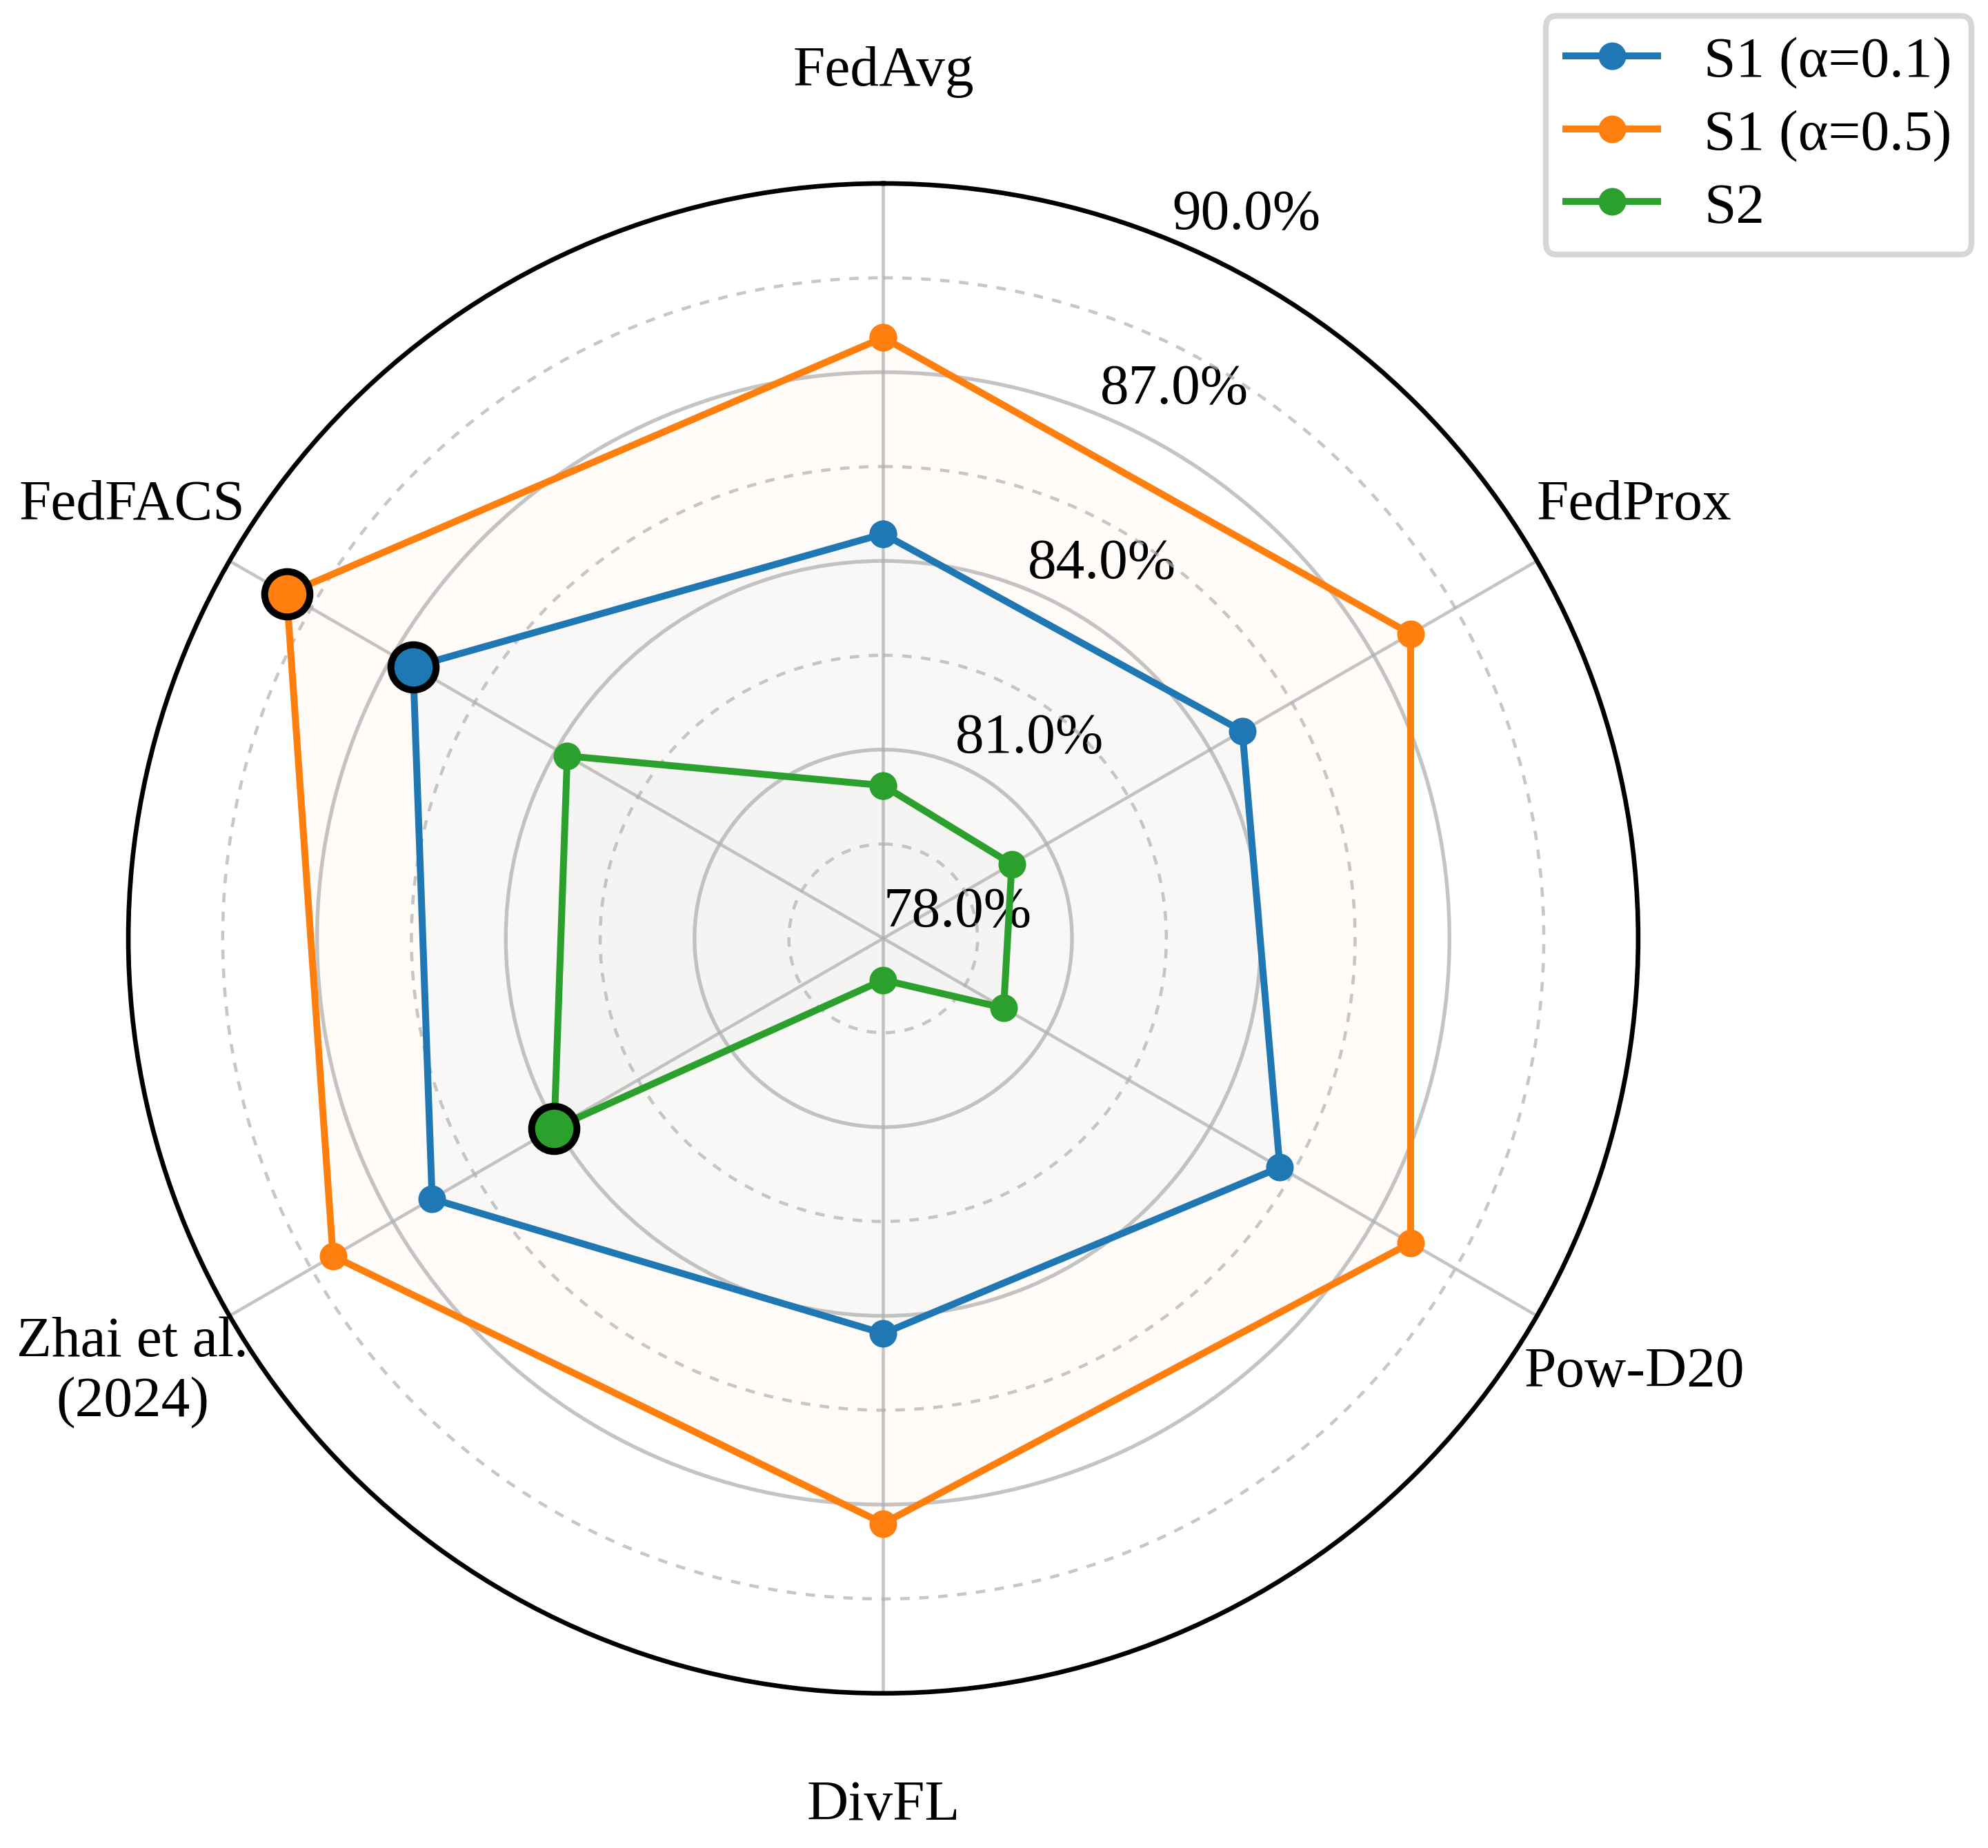
\includegraphics[
        width=\linewidth,
        height=0.3\textheight,
        keepaspectratio
    ]{figures/fig3_c_radar_fmnist.png}
    \vspace{1mm}
    {\footnotesize (c)  FMNIST}
\end{minipage}

\caption{Classification accuracy of FedFACS compared with baseline approaches under different heterogeneous data scenarios, with results presented for CIFAR-10, MNIST, and FMNIST, respectively. The outer axes represent the compared methods, while each curve represents the data heterogeneity scenario; highlighted markers indicate the best-performing method in each scenario.}
\vspace{5mm}

\label{fig:acc_fmnist}
\end{minipage}
\end{figure}


\FloatBarrier

%% Table 3 %%
\begin{table}[!htbp]
\centering
\footnotesize
\setlength{\tabcolsep}{4pt}
\renewcommand{\arraystretch}{1.15}
\setlength{\abovecaptionskip}{2pt}
\setlength{\belowcaptionskip}{4pt}

\caption{Comparison of the required communication rounds for achieving the target accuracy between FedFACS and baseline methods.}
\label{tab:round_cfgA}

\begin{tabular*}{\journalfloatwidth}{@{\extracolsep{\fill}}llcccccc@{}}
\toprule
Dataset & Scenario & FedAvg & FedProx & Pow-D20 & DivFL &
\begin{tabular}[c]{@{}c@{}}Zhai~et~al.\\(2024)\end{tabular} & FedFACS \\
\midrule
CIFAR-10 & S1($\alpha{=}0.1$) & 91 & 197 & 97 & 72 & 44 & \textbf{40} \\
         & S1($\alpha{=}0.5$) & 105 & 87 & 153 & 130 & 62 & \textbf{57} \\
         & S2                 & 135 & 148 & 125 & 200 & 113 & \textbf{110} \\

MNIST    & S1($\alpha{=}0.1$) & 118 & 131 & 100 & \textbf{28} & 68 & 58 \\
         & S1($\alpha{=}0.5$) & 100 & 106 & 94 & \textbf{35} & 73 & 69 \\
         & S2                 & 145 & 169 & 135 & 200 & 116 & \textbf{115} \\

FMNIST   & S1($\alpha{=}0.1$) & 117 & 132 & 115 & 179 & 85 & \textbf{81} \\
         & S1($\alpha{=}0.5$) & 128 & 116 & 124 & 161 & 101 & \textbf{99} \\
         & S2                 & 168 & 186 & 125 & 200 & 108 & \textbf{105} \\
\bottomrule
\end{tabular*}
\end{table}

\FloatBarrier


An overview of the experimental results obtained by FedFACS on CIFAR-10, MNIST, and FMNIST is presented in Table 3 and Fig. 3, illustrating its capability to achieve higher accuracy with fewer communication rounds, while Fig. 4 indicates the cumulative number of participating clients. All the experiments follow configuration A under non-IID settings defined by data partitioning 
scenarios 1 and 2. Each experiment is executed for 200 training rounds to evaluate the global model accuracy under each data distribution. The target accuracy is defined separately for each dataset following the experimental study by Zhai et al. (2024), in addition to the cumulative count of aggregated clients required to achieve this target.

\FloatBarrier

%% imgs fig3 %%
\begin{figure}[!p]
\centering

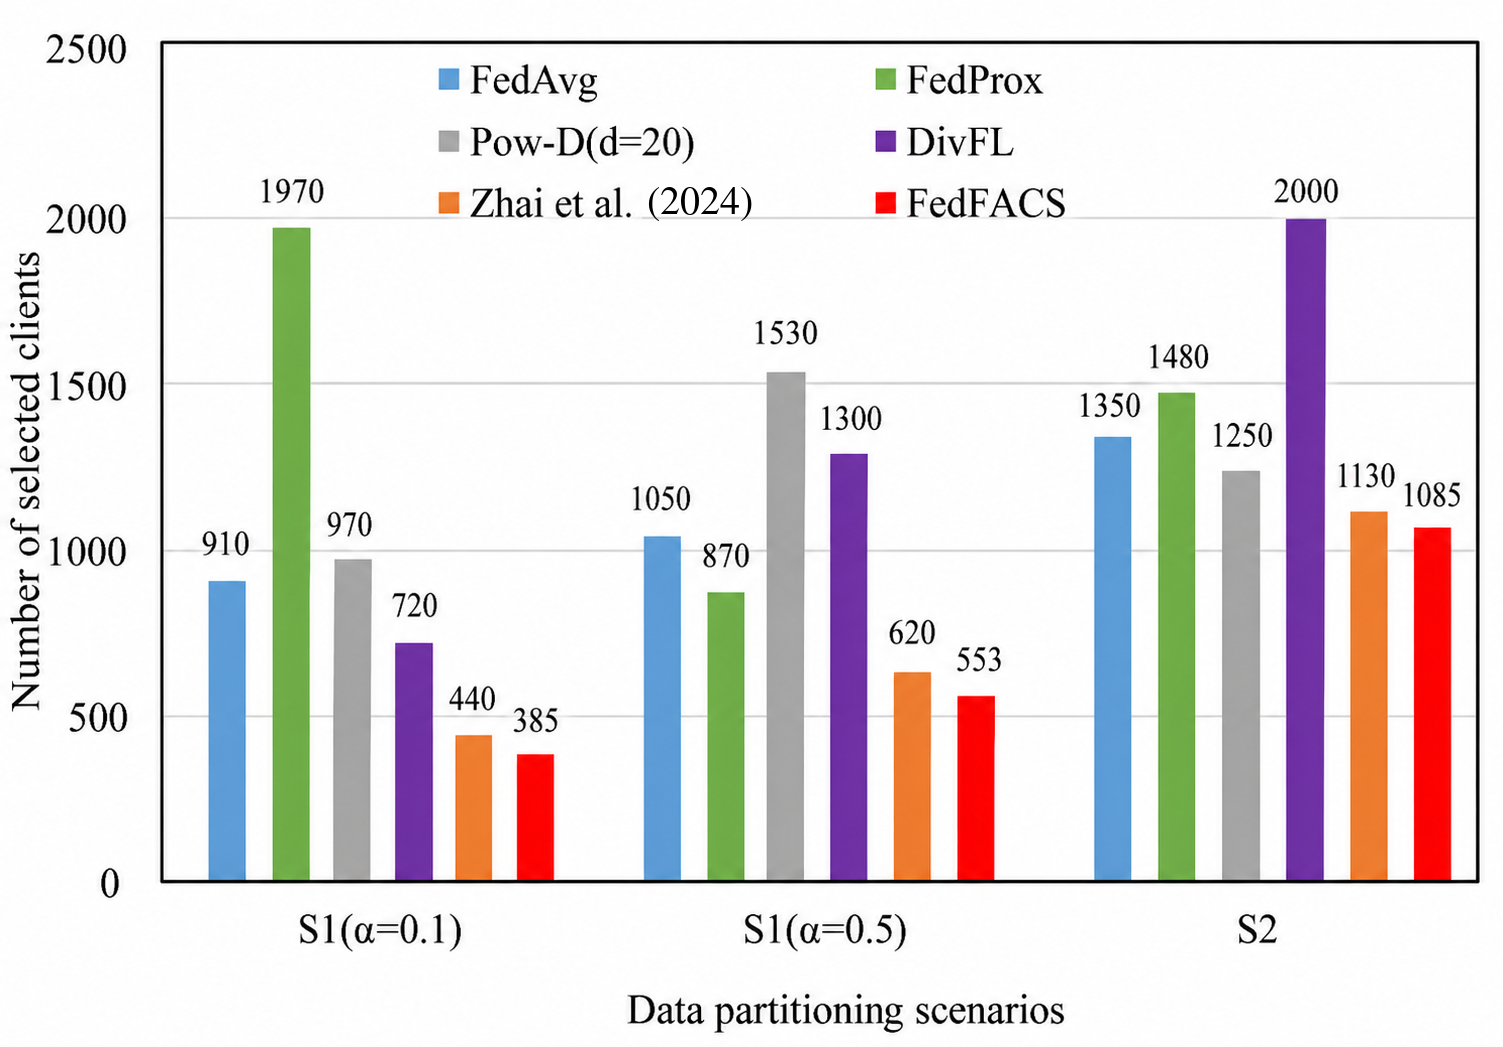
\includegraphics[width=0.61\textwidth]{figures/fig4__a.png}
\par\vspace{-2mm}
{\footnotesize (a) CIFAR-10}

\vspace{2mm}

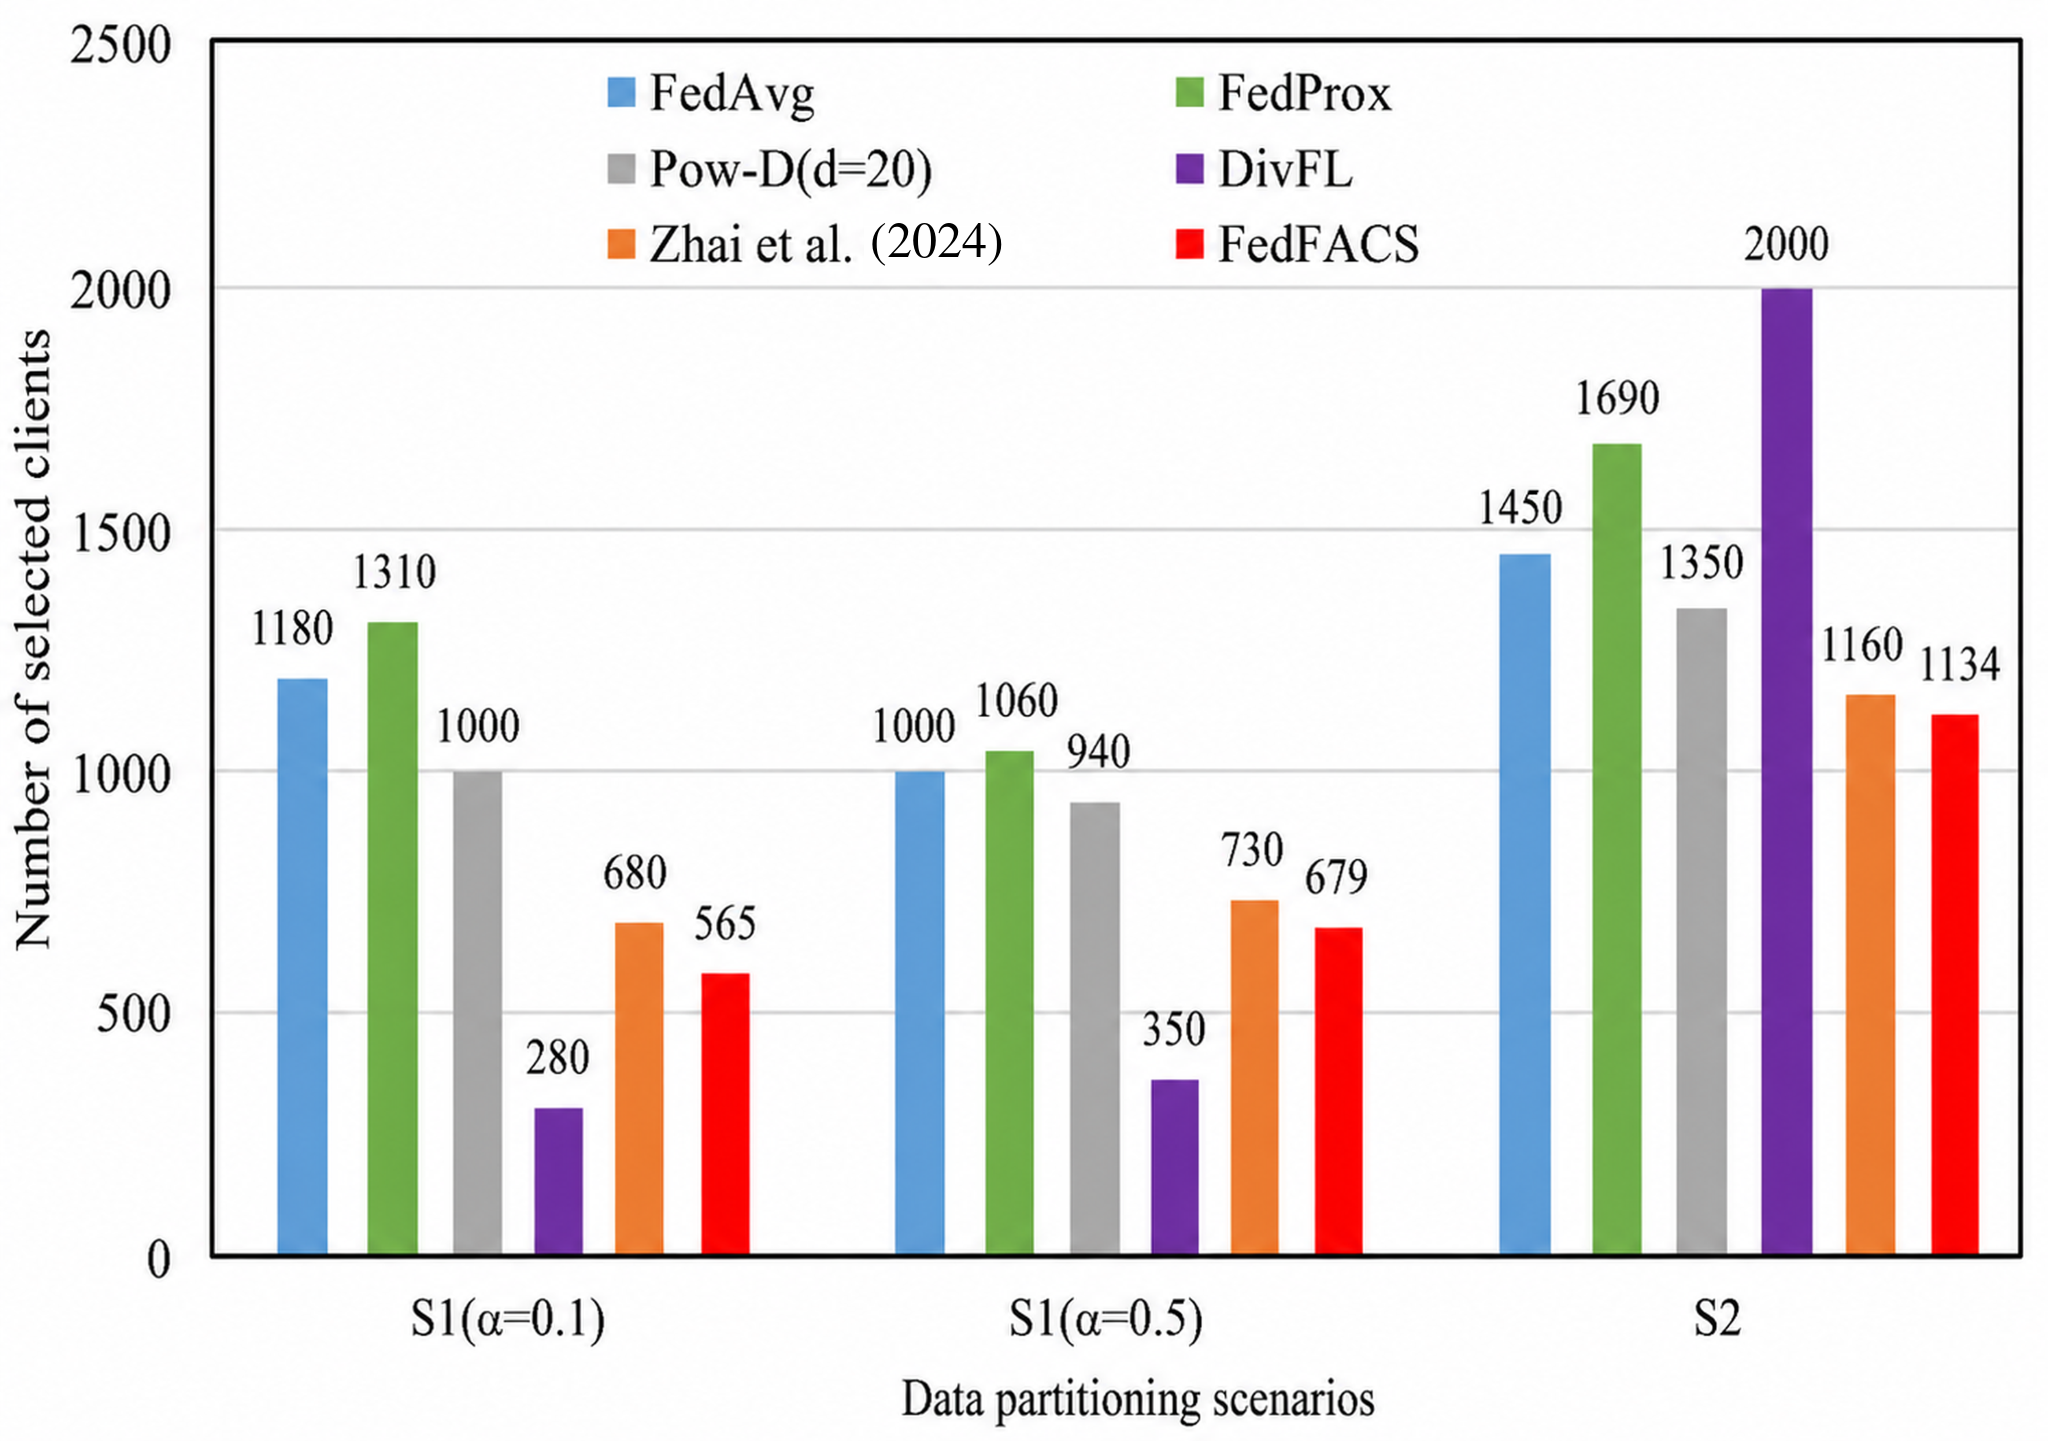
\includegraphics[width=0.61\textwidth]{figures/fig4__b.png}
\par\vspace{-2mm}
{\footnotesize (b) MNIST}

\vspace{2mm}

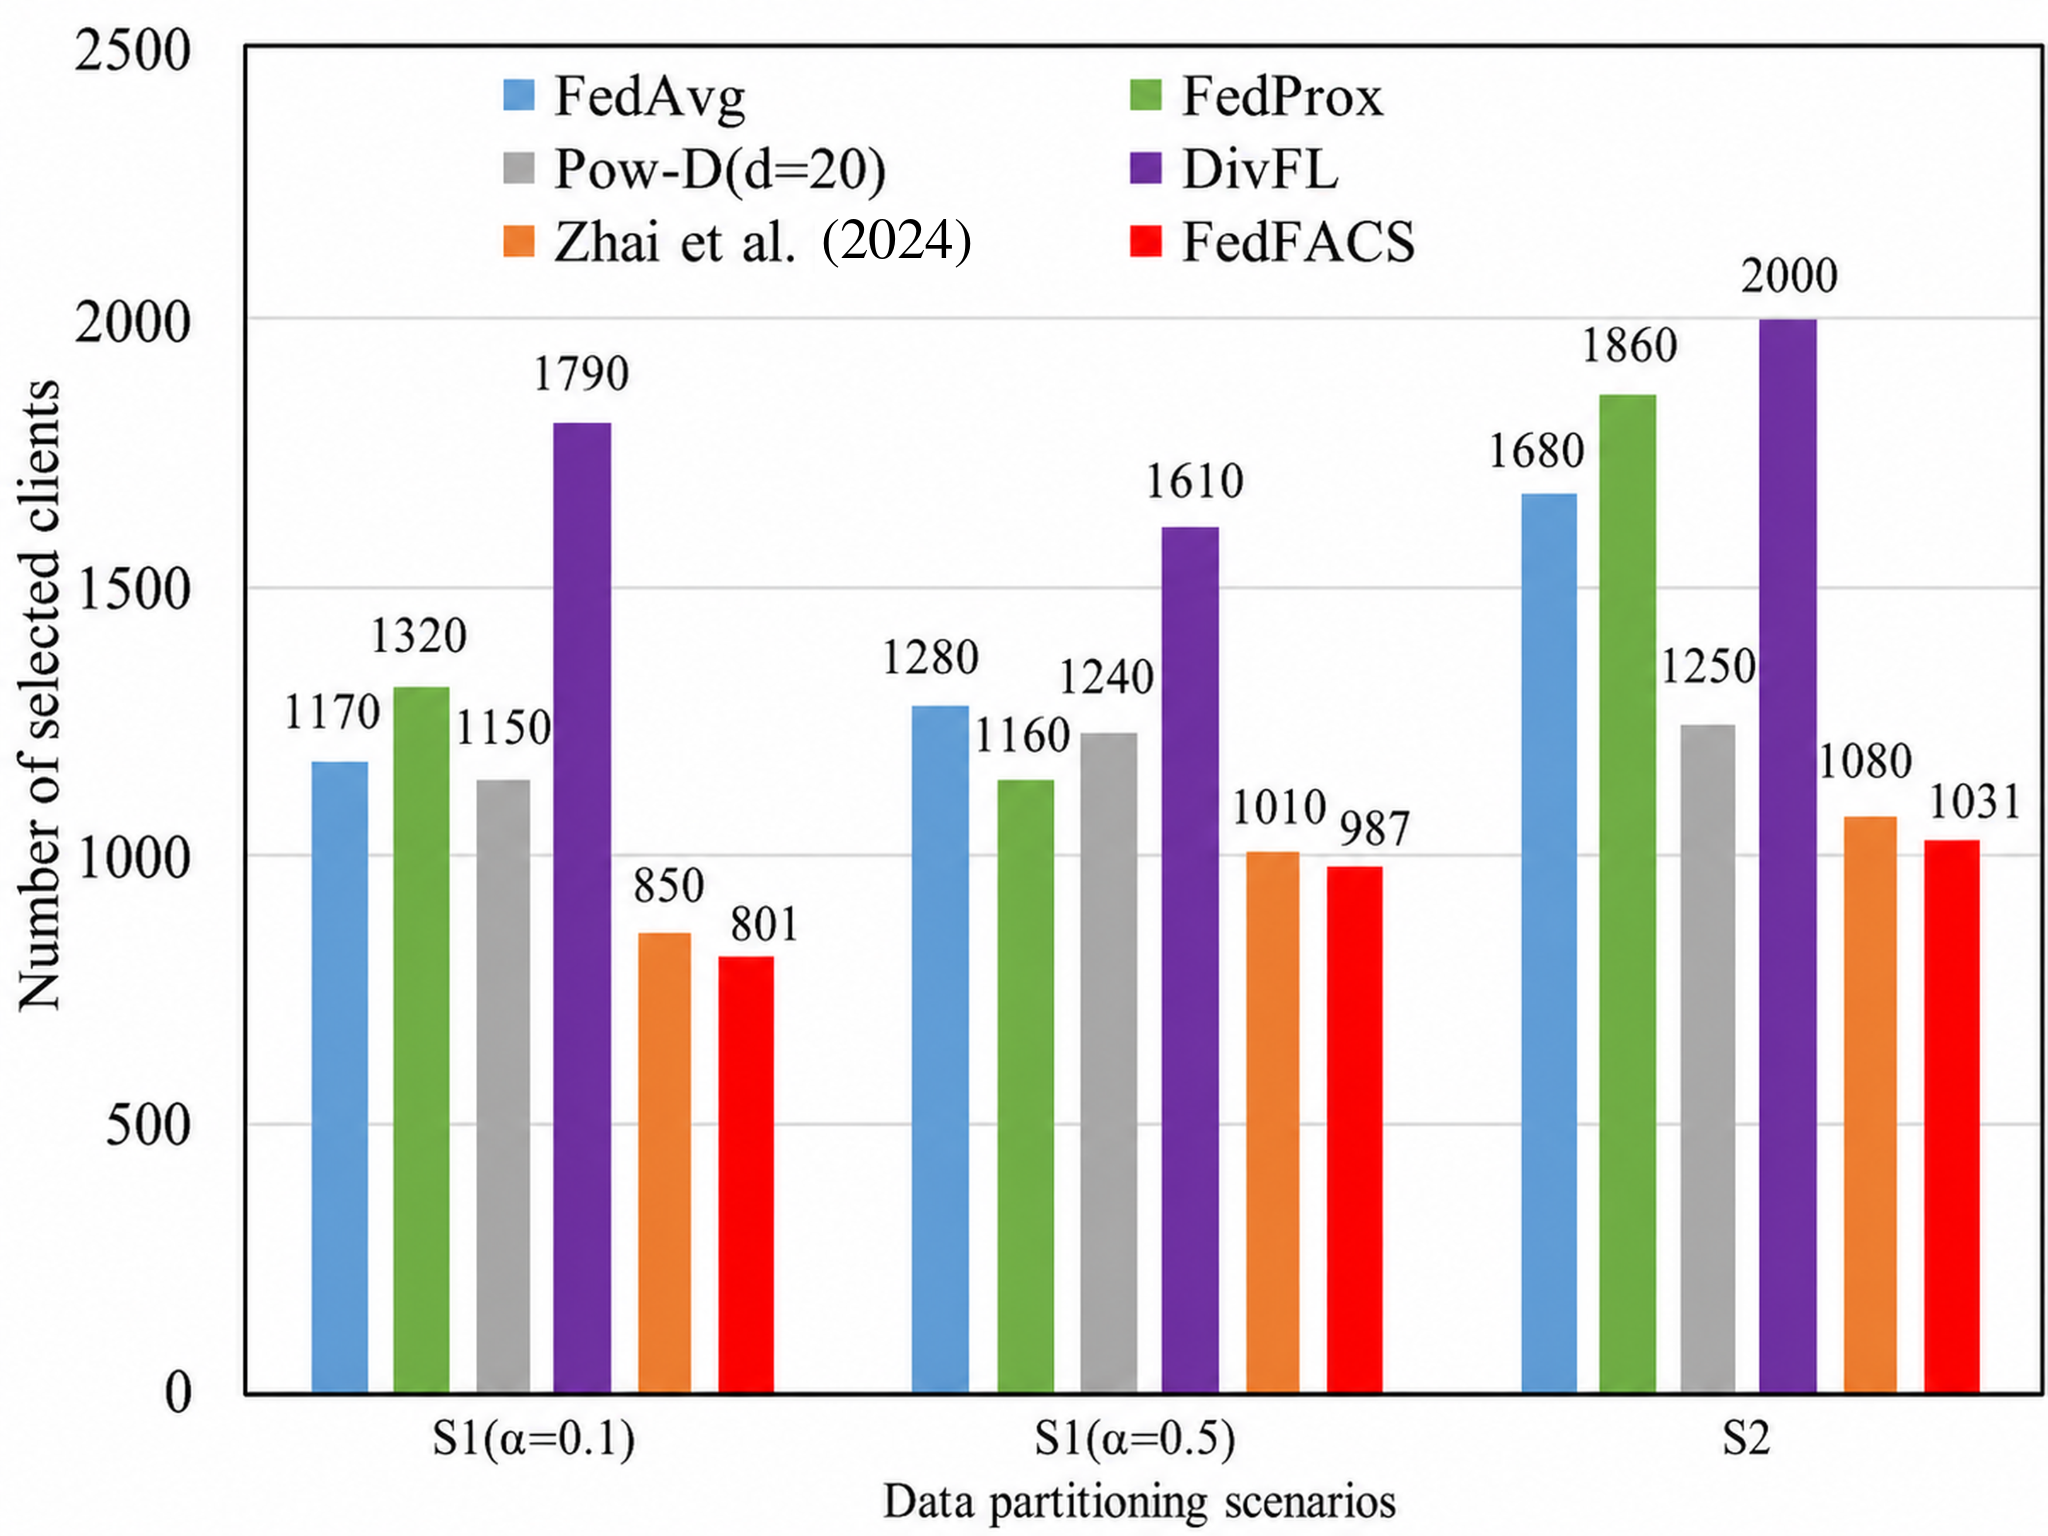
\includegraphics[width=0.61\textwidth]{figures/fig4__c.png}
\par\vspace{-2mm}
{\footnotesize (c) FMNIST}

\vspace{1mm}

\caption{Cumulative number of selected clients required to achieve the target accuracy under heterogeneous data conditions in Scenarios 1 and 2 for (a) CIFAR-10, (b) MNIST, and (c) FMNIST.}
\label{fig:clients_required}

\end{figure}


\begin{figure}[!htbp]
\noindent
\begin{minipage}{\linewidth}
\centering

\begin{minipage}[t]{0.32\linewidth}
    \centering
    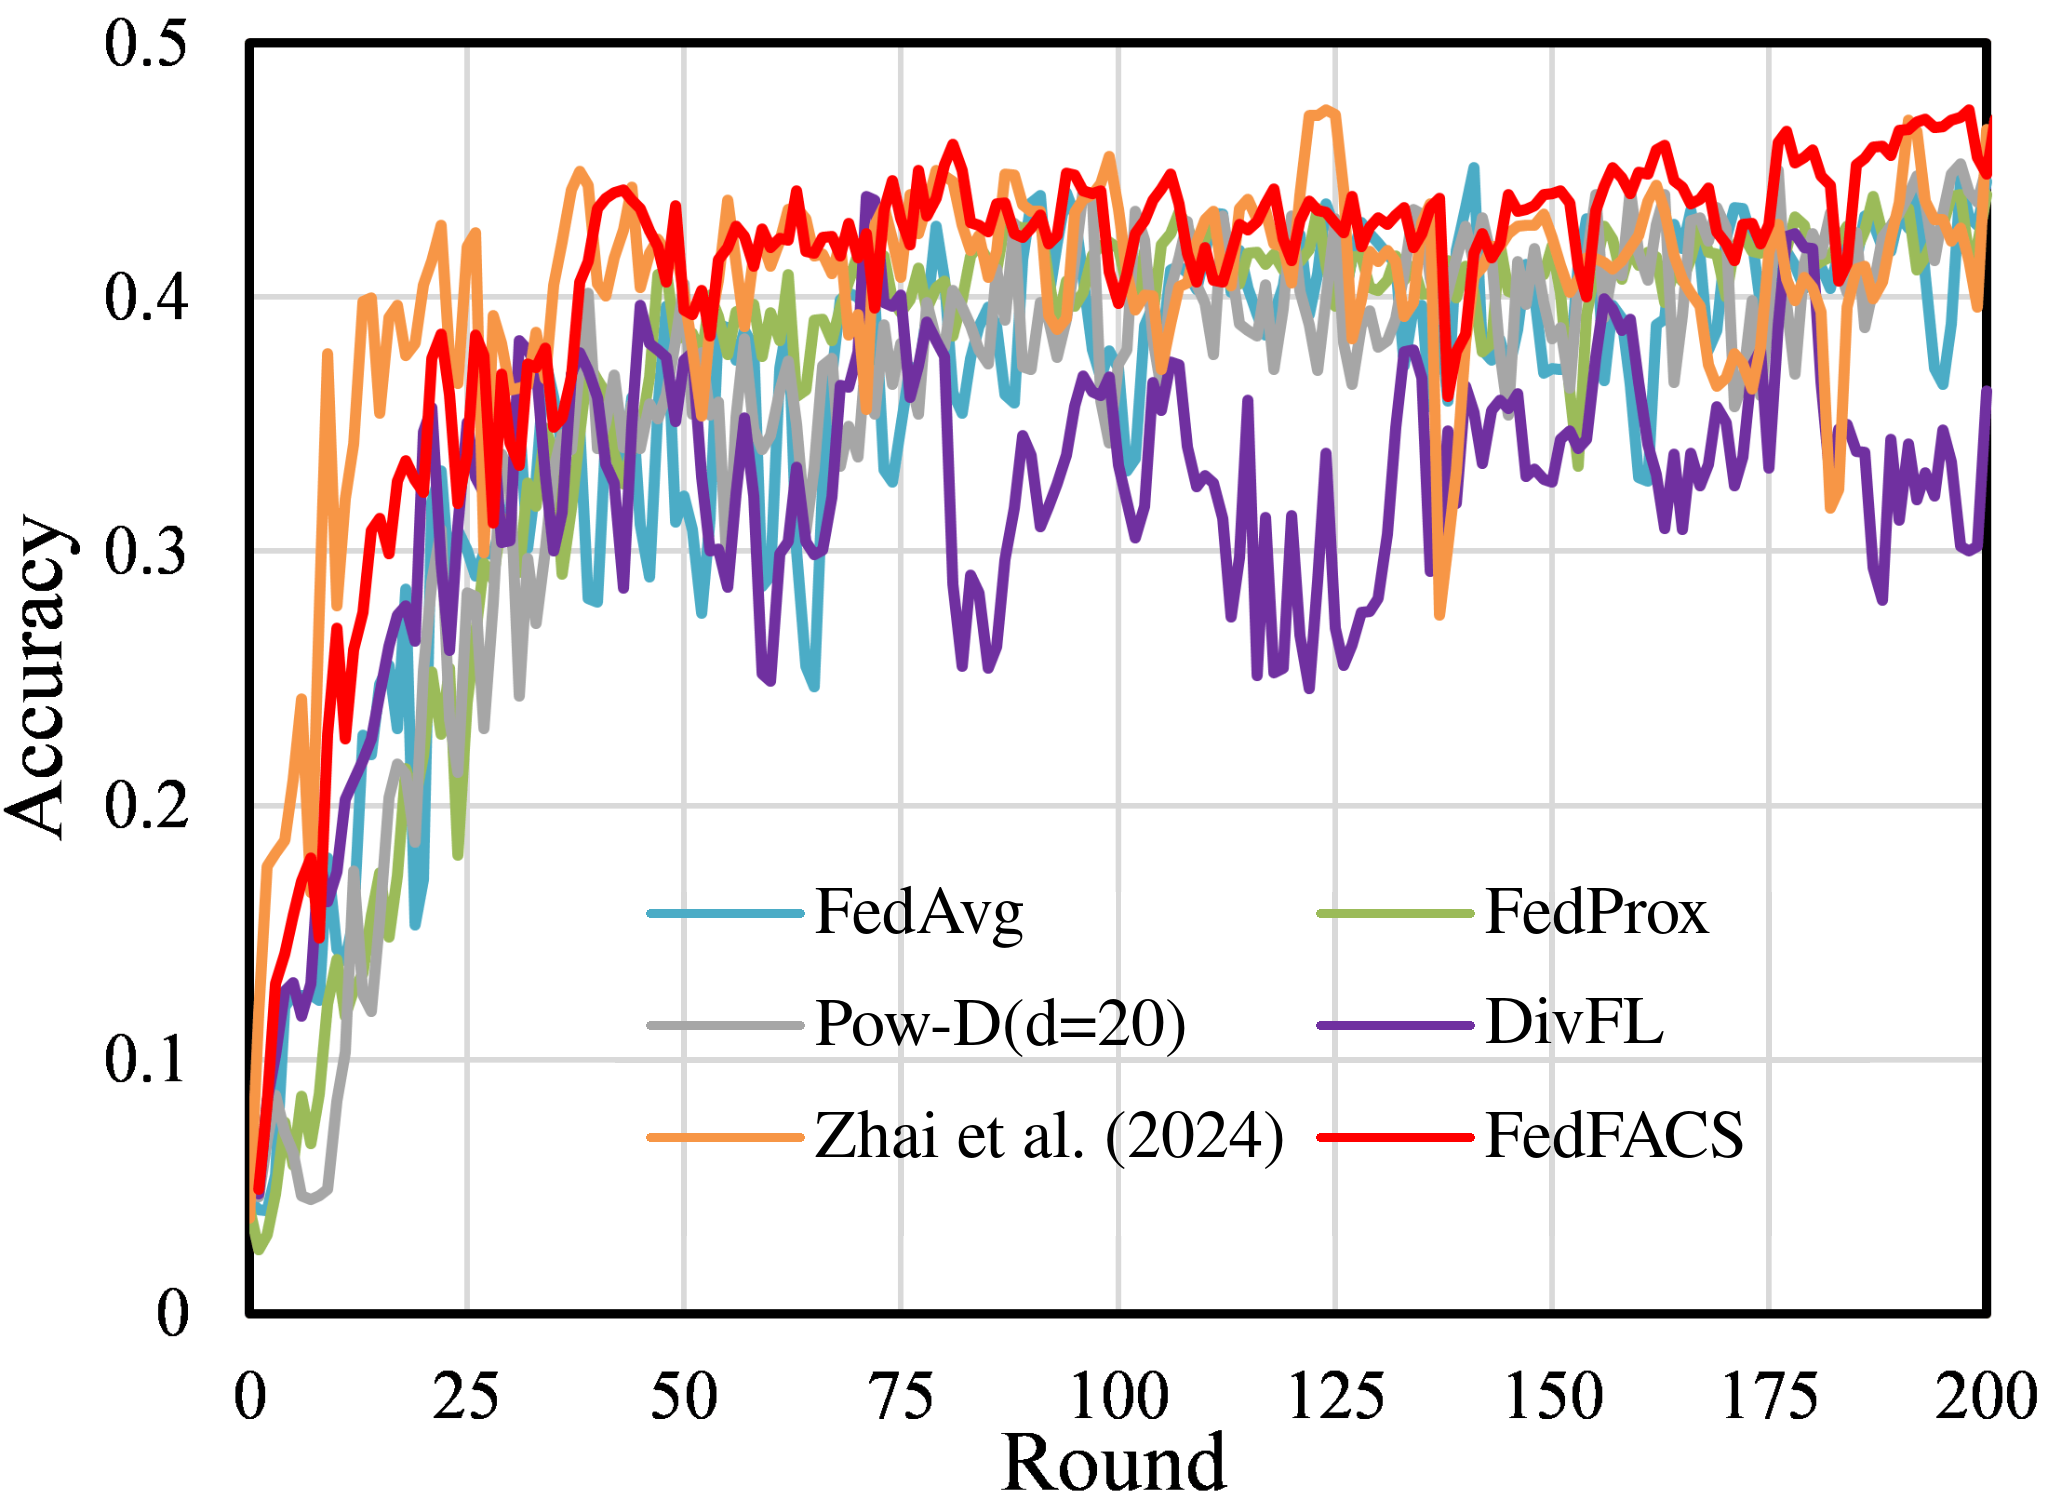
\includegraphics[
        width=\linewidth,
        height=0.3\textheight,
        keepaspectratio
    ]{figures/fig5__a.png}
    \vspace{1mm}
    {\footnotesize (a) Scenario 1 ($\alpha=0.1$)}
\end{minipage}
\hfill
\begin{minipage}[t]{0.32\linewidth}
    \centering
    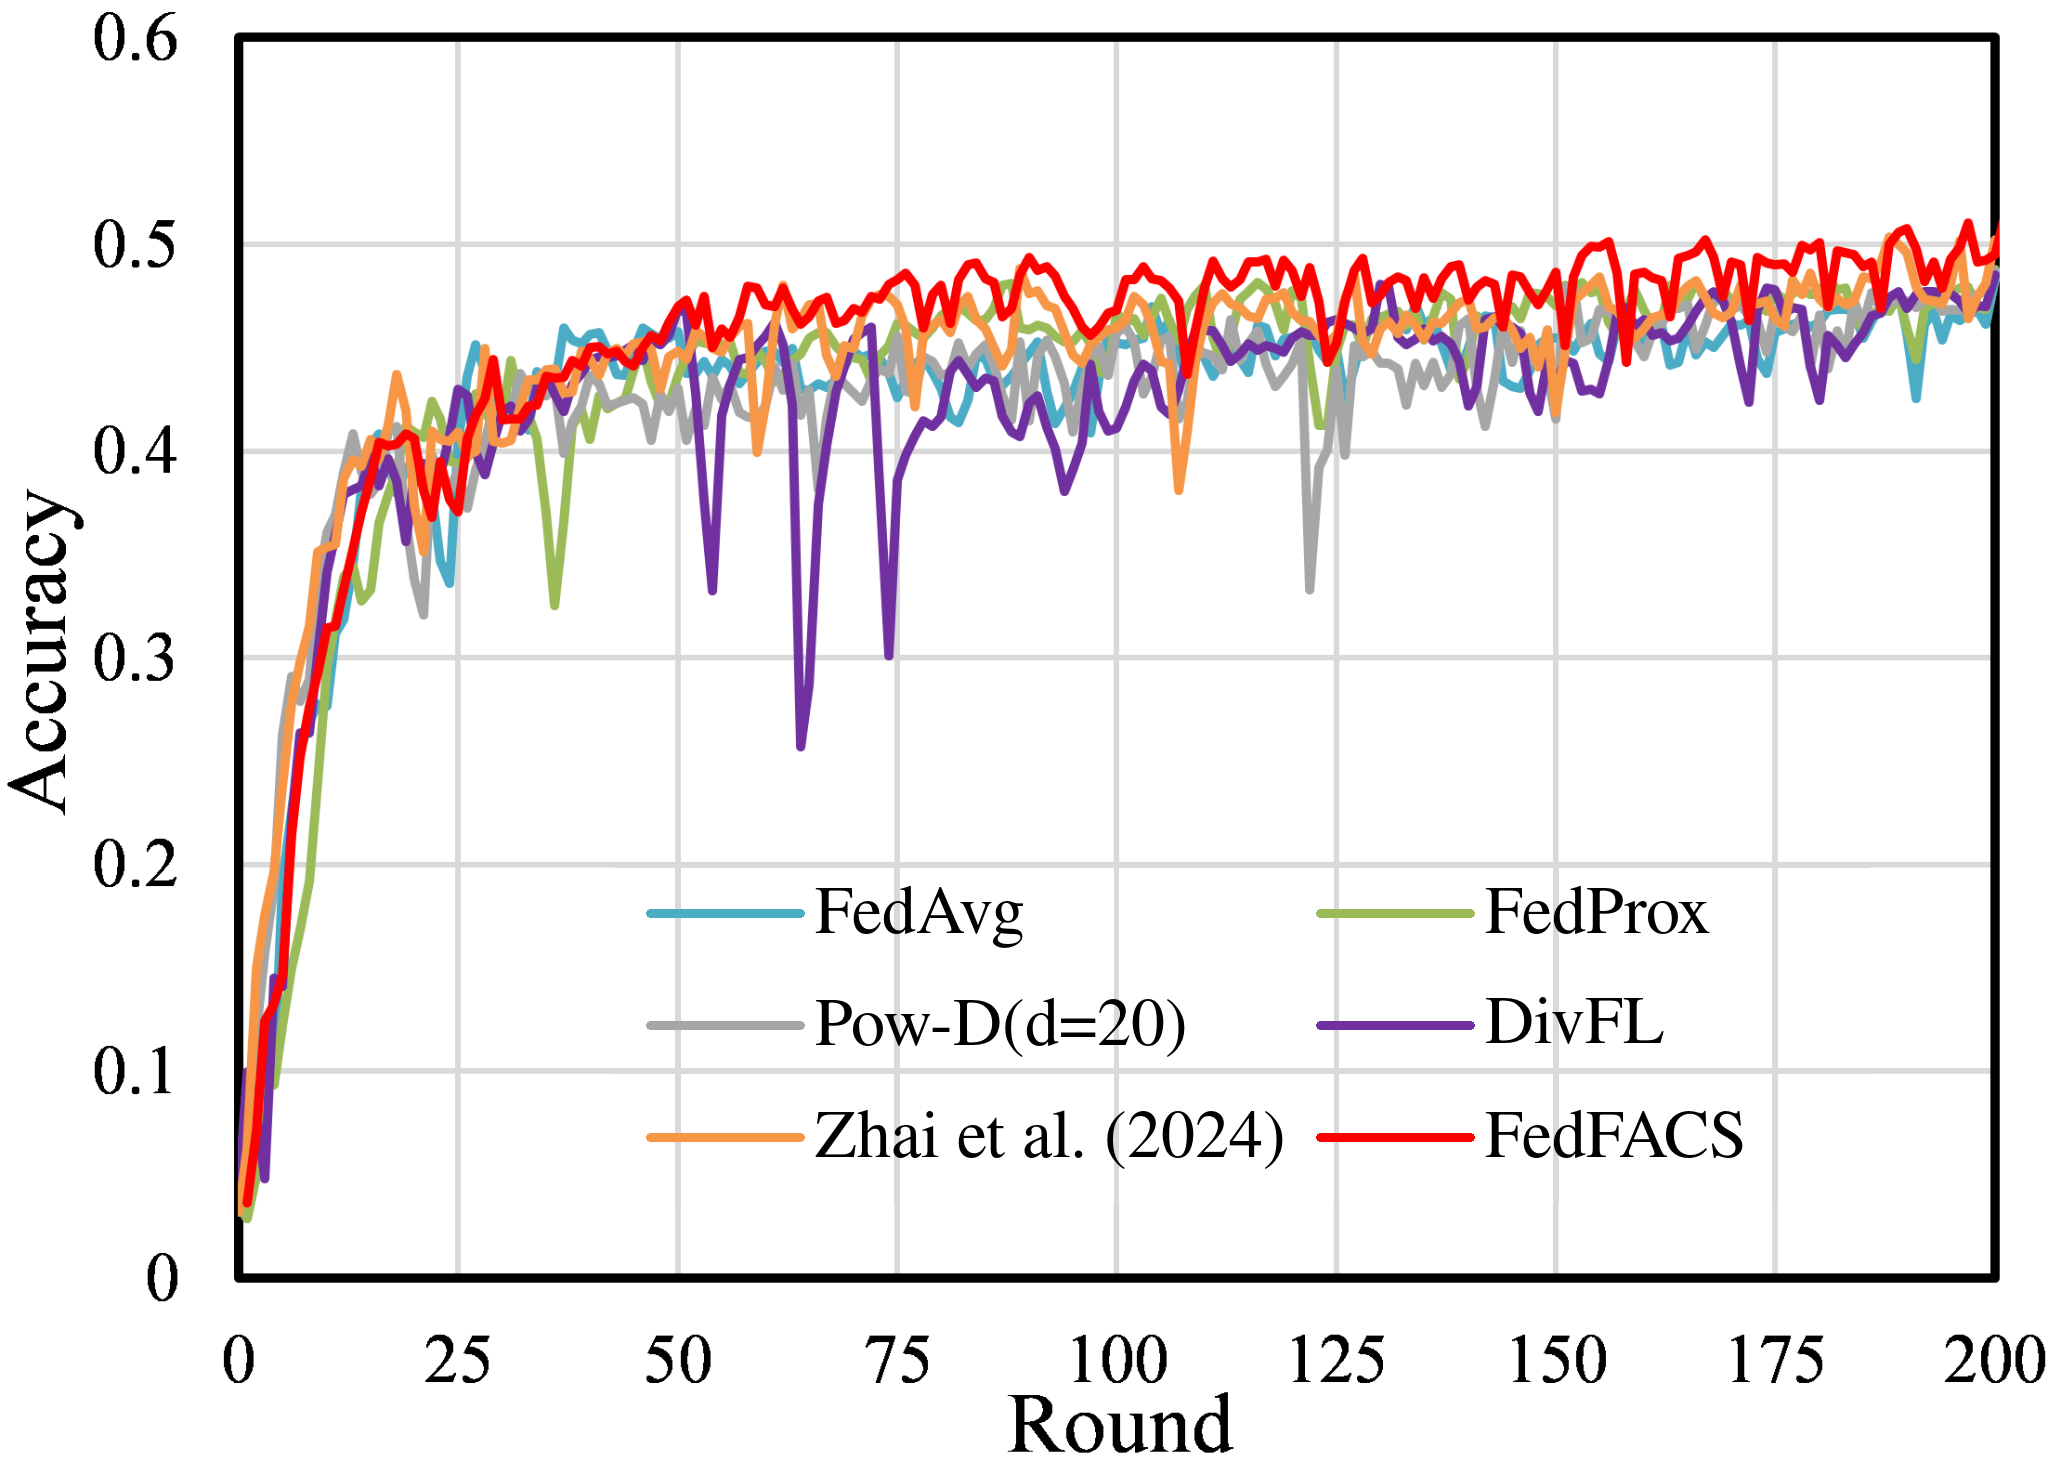
\includegraphics[
        width=\linewidth,
        height=0.3\textheight,
        keepaspectratio
    ]{figures/fig5__b.png}
    \vspace{1mm}
    {\footnotesize (b) Scenario 1 ($\alpha=0.5$)}
\end{minipage}
\hfill
\begin{minipage}[t]{0.32\linewidth}
    \centering
    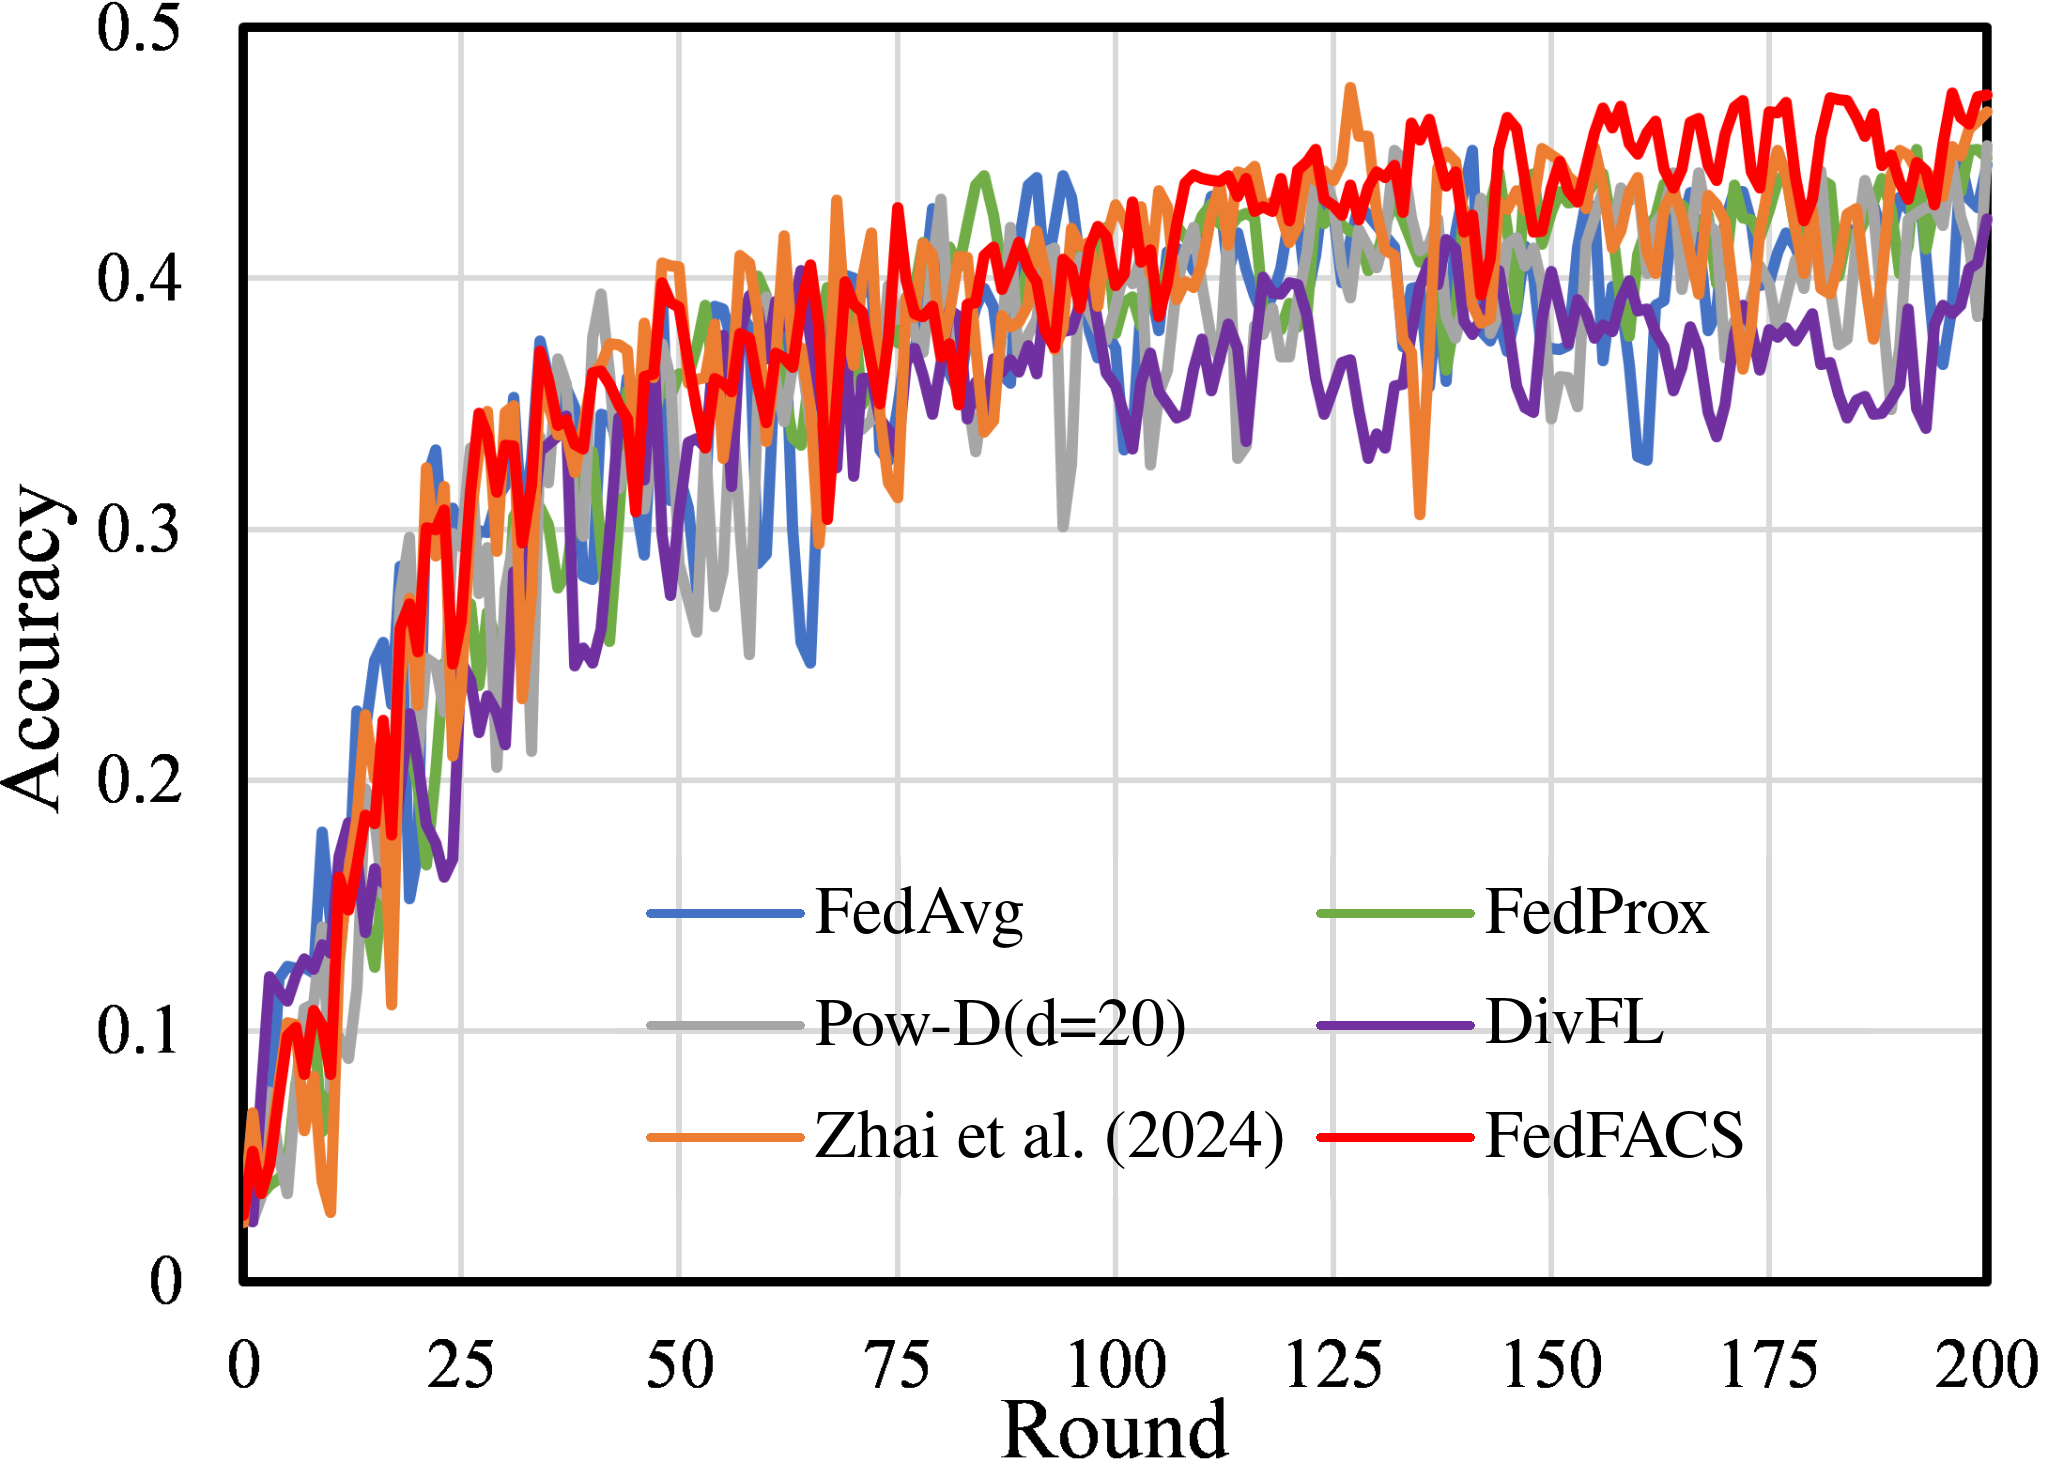
\includegraphics[
        width=\linewidth,
        height=0.3\textheight,
        keepaspectratio
    ]{figures/fig5__c.png}
    \vspace{1mm}
    {\footnotesize (c) Scenario 2}
\end{minipage}

\caption{Accuracy comparison under heterogeneous data conditions in Scenarios 1 and 2 on CIFAR-10.}
\label{fig:acc_cifar10}
\end{minipage}
\end{figure}


\begin{figure}[!htbp]
\noindent
\begin{minipage}{\linewidth}
\centering

\begin{minipage}[t]{0.32\linewidth}
    \centering
    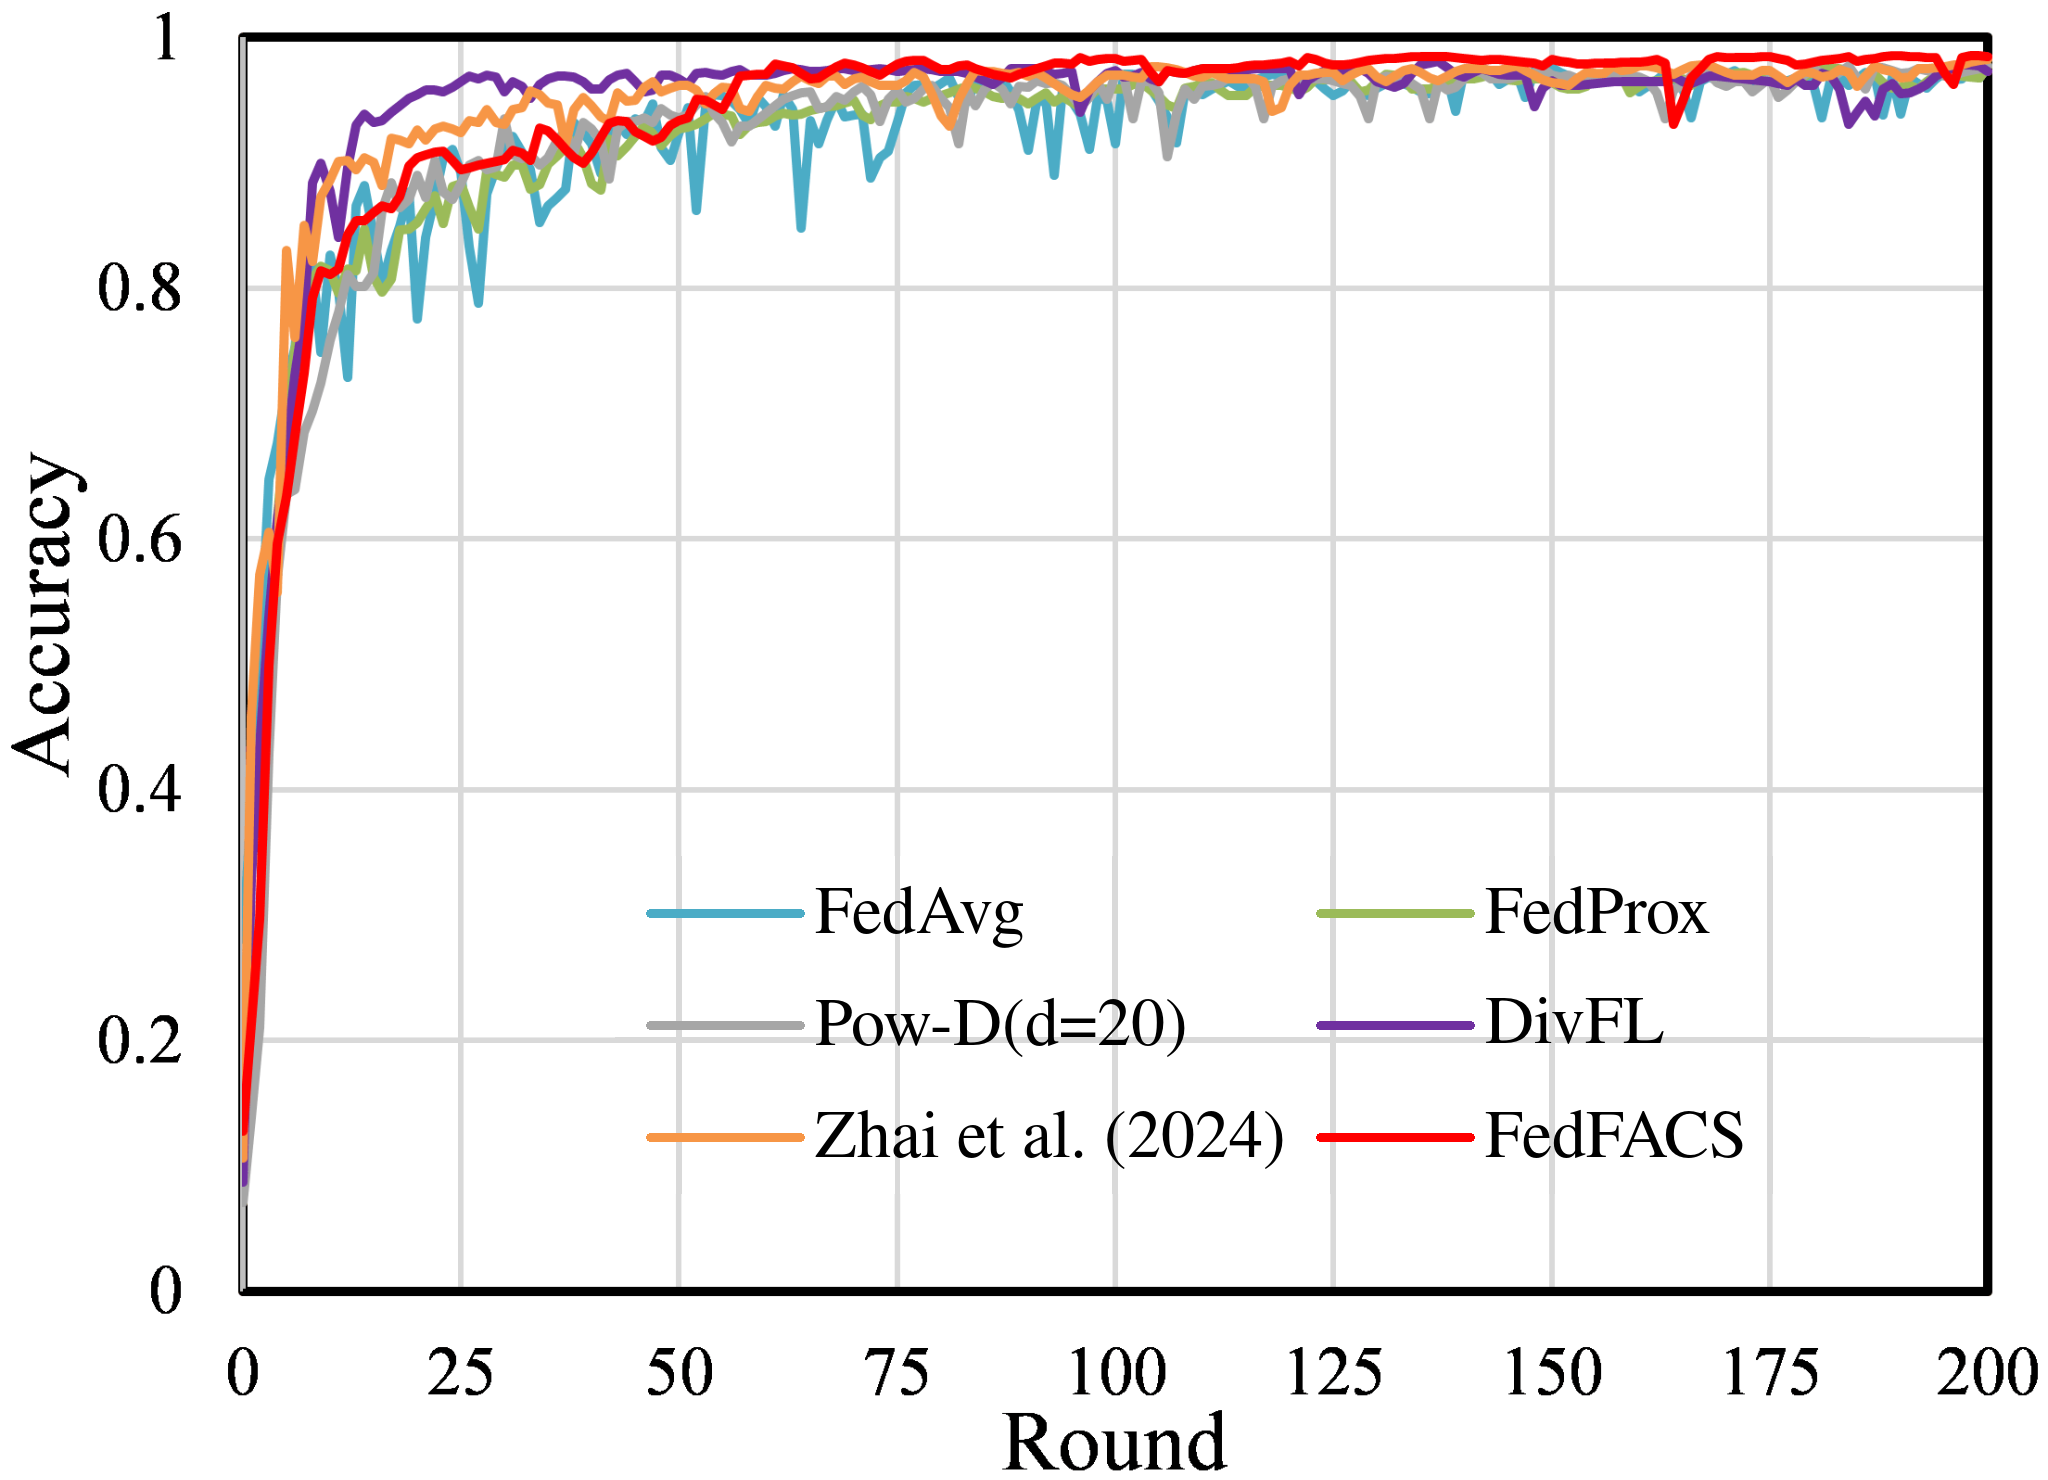
\includegraphics[
        width=\linewidth,
        height=0.3\textheight,
        keepaspectratio
    ]{figures/fig6__a.png}
    \vspace{1mm}
    {\footnotesize (a) Scenario 1 ($\alpha=0.1$)}
\end{minipage}
\hfill
\begin{minipage}[t]{0.32\linewidth}
    \centering
    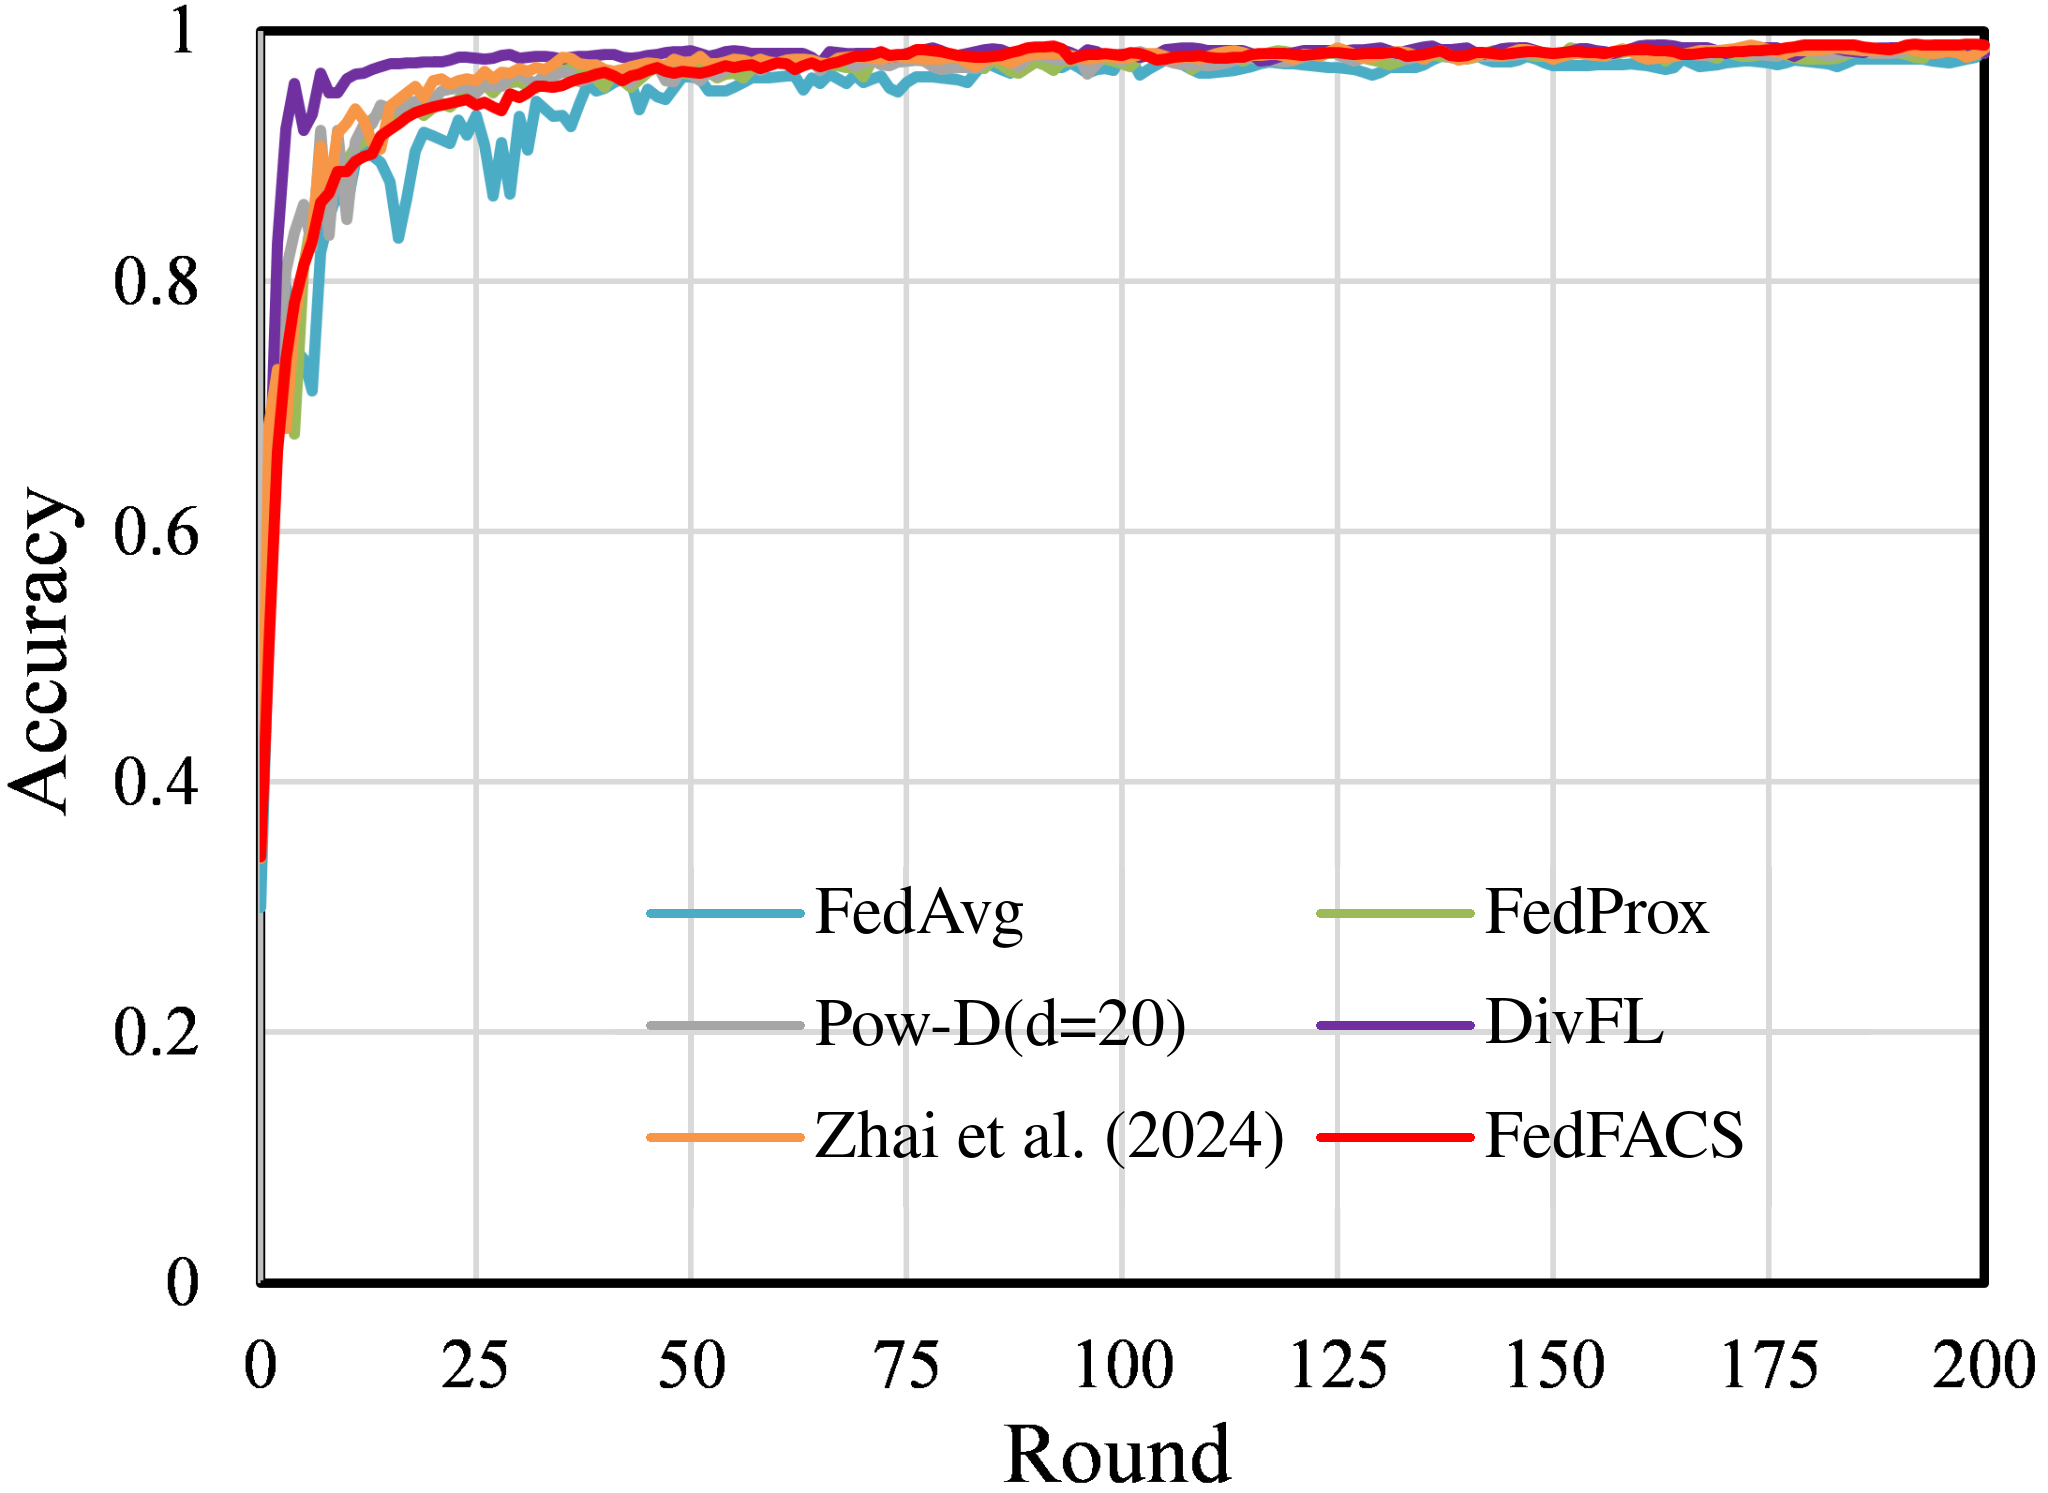
\includegraphics[
        width=\linewidth,
        height=0.3\textheight,
        keepaspectratio
    ]{figures/fig6__b.png}
    \vspace{1mm}
    {\footnotesize (b) Scenario 1 ($\alpha=0.5$)}
\end{minipage}
\hfill
\begin{minipage}[t]{0.32\linewidth}
    \centering
    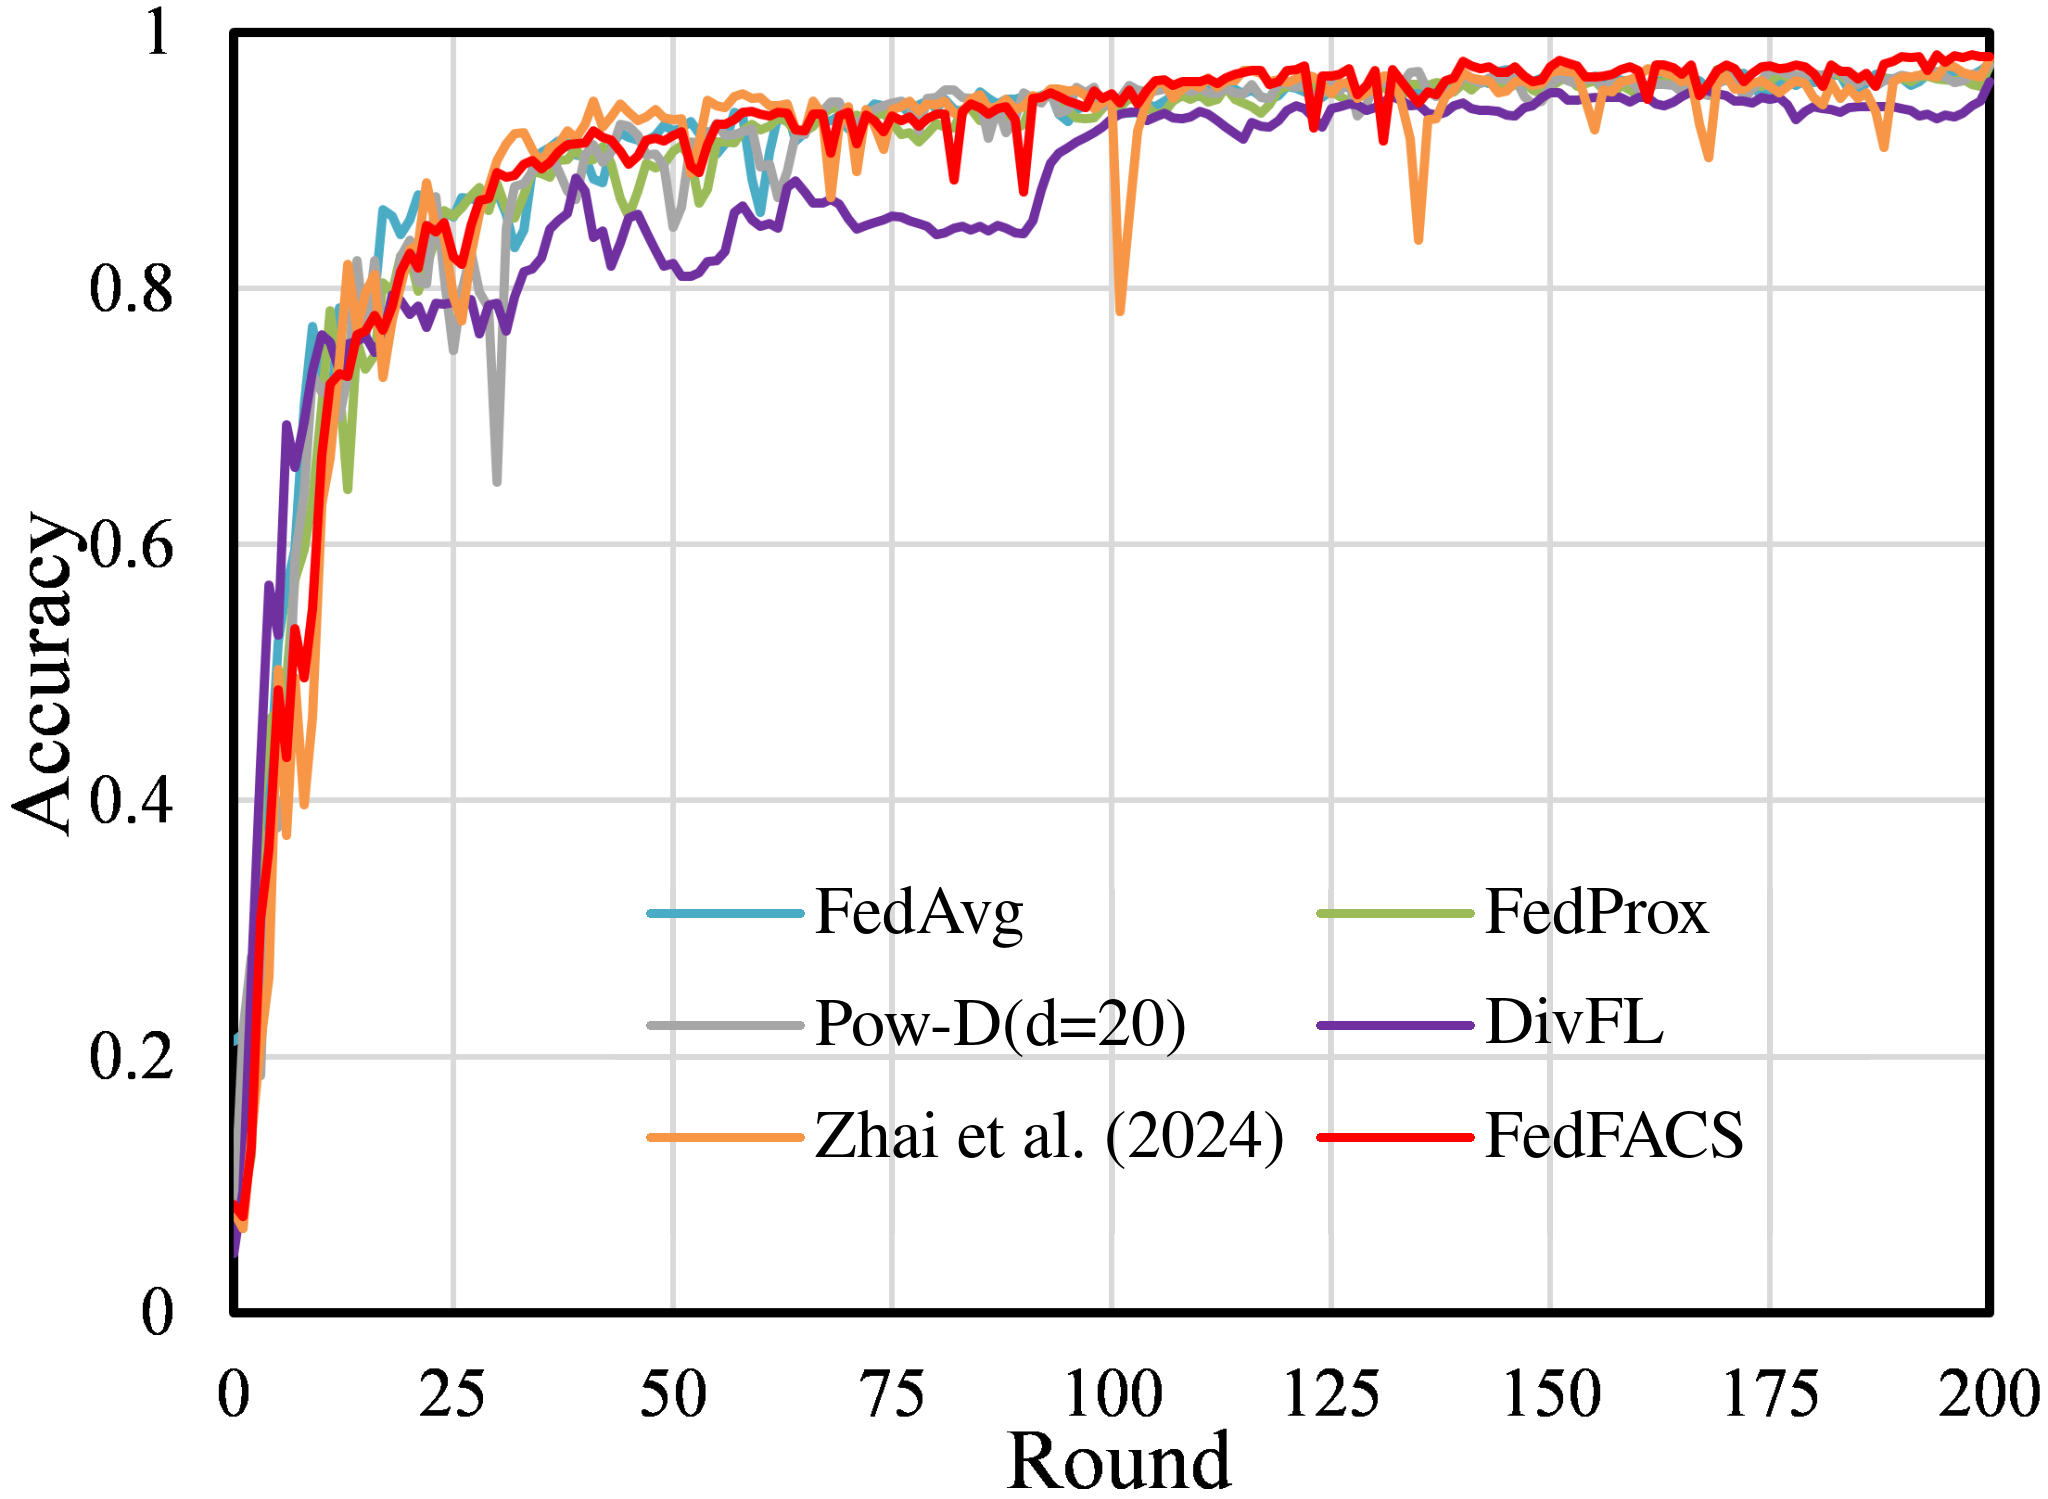
\includegraphics[
        width=\linewidth,
        height=0.3\textheight,
        keepaspectratio
    ]{figures/fig6__c.png}
    \vspace{1mm}
    {\footnotesize (c) Scenario 2}
\end{minipage}

\caption{Accuracy comparison under heterogeneous data conditions in Scenarios 1 and 2 on MNIST.}
\label{fig:acc_mnist}
\end{minipage}
\end{figure}



For the CIFAR-10 dataset, FedFACS achieves accuracies of 47.07\%, 51.12\%, and 47.33\% after 200 training rounds under different data partitioning conditions as illustrated in Fig. 5. FedFACS achieves the best classification accuracy among the baseline methods by 0.48\%, 0.89\%, and 0.67\% increases over the best-performing method. Moreover, Table 3 reports the communication overhead in terms of communication round count required to achieve a predefined accuracy, where the target accuracies were configured to 44\%, 48\%, and 44\% across the three data distribution scenarios.


In comparison with the baseline approaches, FedFACS accelerates convergence, requiring approximately 40, 57, and 110 rounds to attain the target accuracy under the three non-IID conditions, respectively, representing reductions of approximately 9\%, 8\%, and 2.6\% in communication rounds compared with Zhai et al. (2024). The observed reduction in communication rounds depends on the level of data skewness across the evaluated scenarios, reflecting the effectiveness of the adaptive control mechanism. The 9\% and 8\% improvements are achieved in more stable scenarios, where FedFACS rapidly identifies informative clients and eliminates redundant communication rounds, while in the more challenging scenario with a 2.6\% improvement, the convergence slows due to severe data heterogeneity where clients hold underrepresented classes which leads to a slower aggregation process to ensure stable convergence over additional rounds. In addition, FedFACS reduces the communication overhead not only by achieving the target accuracy in fewer communication rounds, but also by requiring a lower cumulative count of clients involved in aggregation, with approximately $4\%-12.5\%$ fewer clients than the best-performing baseline as demonstrated in Fig. 4(a). As a result, the overall communication overhead associated with data transmission is reduced. 

Furthermore, FedFACS records the highest average accuracies of 98.52\%, 98.91\%, and 98.11\%, with corresponding improvements of 0.27\%, 0.31\%, and 0.22\% over the best-performing method under the three data distribution conditions, as shown in Fig. 6. Moreover, FedFACS attains the predefined target accuracies of 97\%, 98\%, and 97\% within approximately 58, 69, and 115 communication rounds as presented in Table 3, demonstrating a reduction in communication overhead compared with Zhai et al. (2024) for the first two distribution conditions by 14.7\% and 5.4\%, while selecting approximately $7\%-17\%$ fewer clients as illustrated in Fig. 4(b). However, no much improvement is observed under the data partitioning of scenario 2. In addition, DivFL is 2x faster than the proposed framework with fewer selected clients under the first data distribution scenario. Nevertheless, FedFACS sacrifices communication efficiency to ensure fairness and achieves higher final accuracy compared with DivFL by 1.19\%, 0.74\%, and 1.98\% across the three distribution conditions.



Finally, FedFACS achieves the highest average accuracies of 86.63\%, 88.95\%, and 83.08\% under varying data distribution conditions. Relative to the best baseline approach, these outcomes show increases of 0.35\% and 0.85\% under the first two distribution conditions, while a slight decrease of 0.2\% in the third condition, as illustrated in Fig. 7. Furthermore, the proposed framework reaches the predefined target accuracies of 84\%, 87\%, and 80\% within 81, 99, and 105 corresponding training rounds. This demonstrates an enhanced communication efficiency compared with the best-performing baseline, Zhai et al. (2024) by selecting $2.3\%-5.8\%$ fewer clients, as shown in Fig. 4(c) and requiring approximately 4.7\%, 2\%, and 2.2\% fewer communication rounds as presented in Table 3. 

%%%%%%%%%%%%%%%%%%%%%%%%%%%%%%%%%%%%%%%%%%%%%%%%%%%%%%
% Three Images
%%%%%%%%%%%%%%%%%%%%%%%%%%%%%%%%%%%%%%%%%%%%%%%%%%%%%%

\noindent
\begin{minipage}{\linewidth}
\centering

\begin{minipage}[t]{0.32\linewidth}
    \vspace{0pt}\centering
    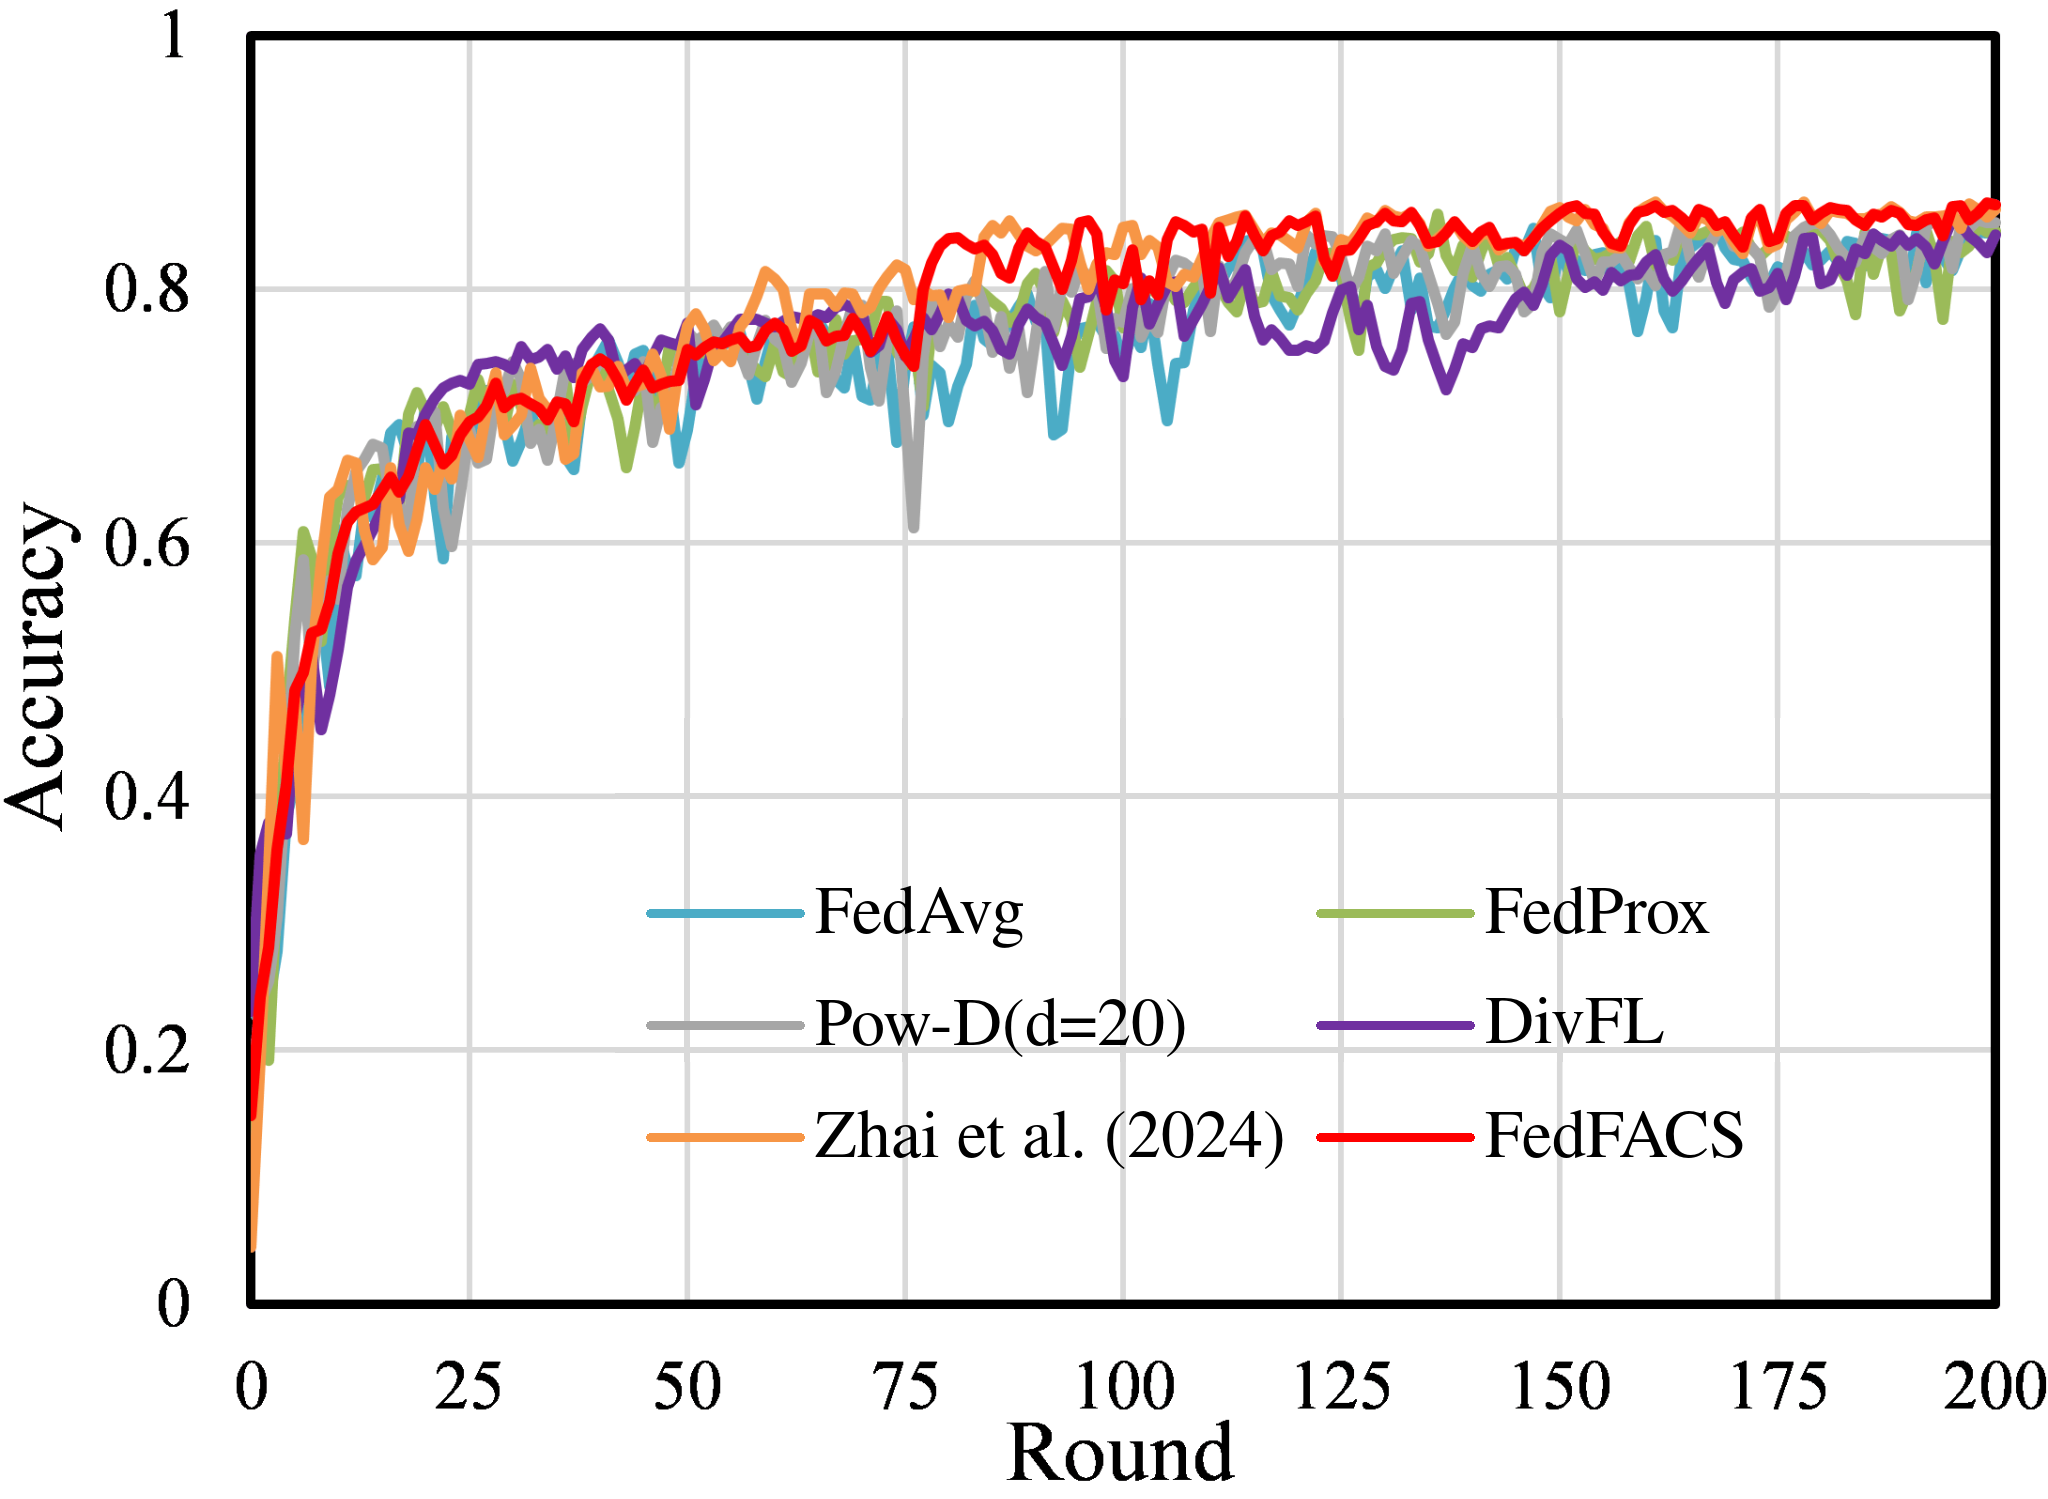
\includegraphics[
        width=\linewidth,
        height=4.15cm,
        keepaspectratio
    ]{figures/fig7__a.png}
    \par\vspace{0.5mm}
    {\fontsize{7pt}{8pt}\selectfont
    (a) Scenario 1 ($\alpha=0.1$)}
\end{minipage}
\hfill
\begin{minipage}[t]{0.32\linewidth}
    \vspace{0pt}\centering
    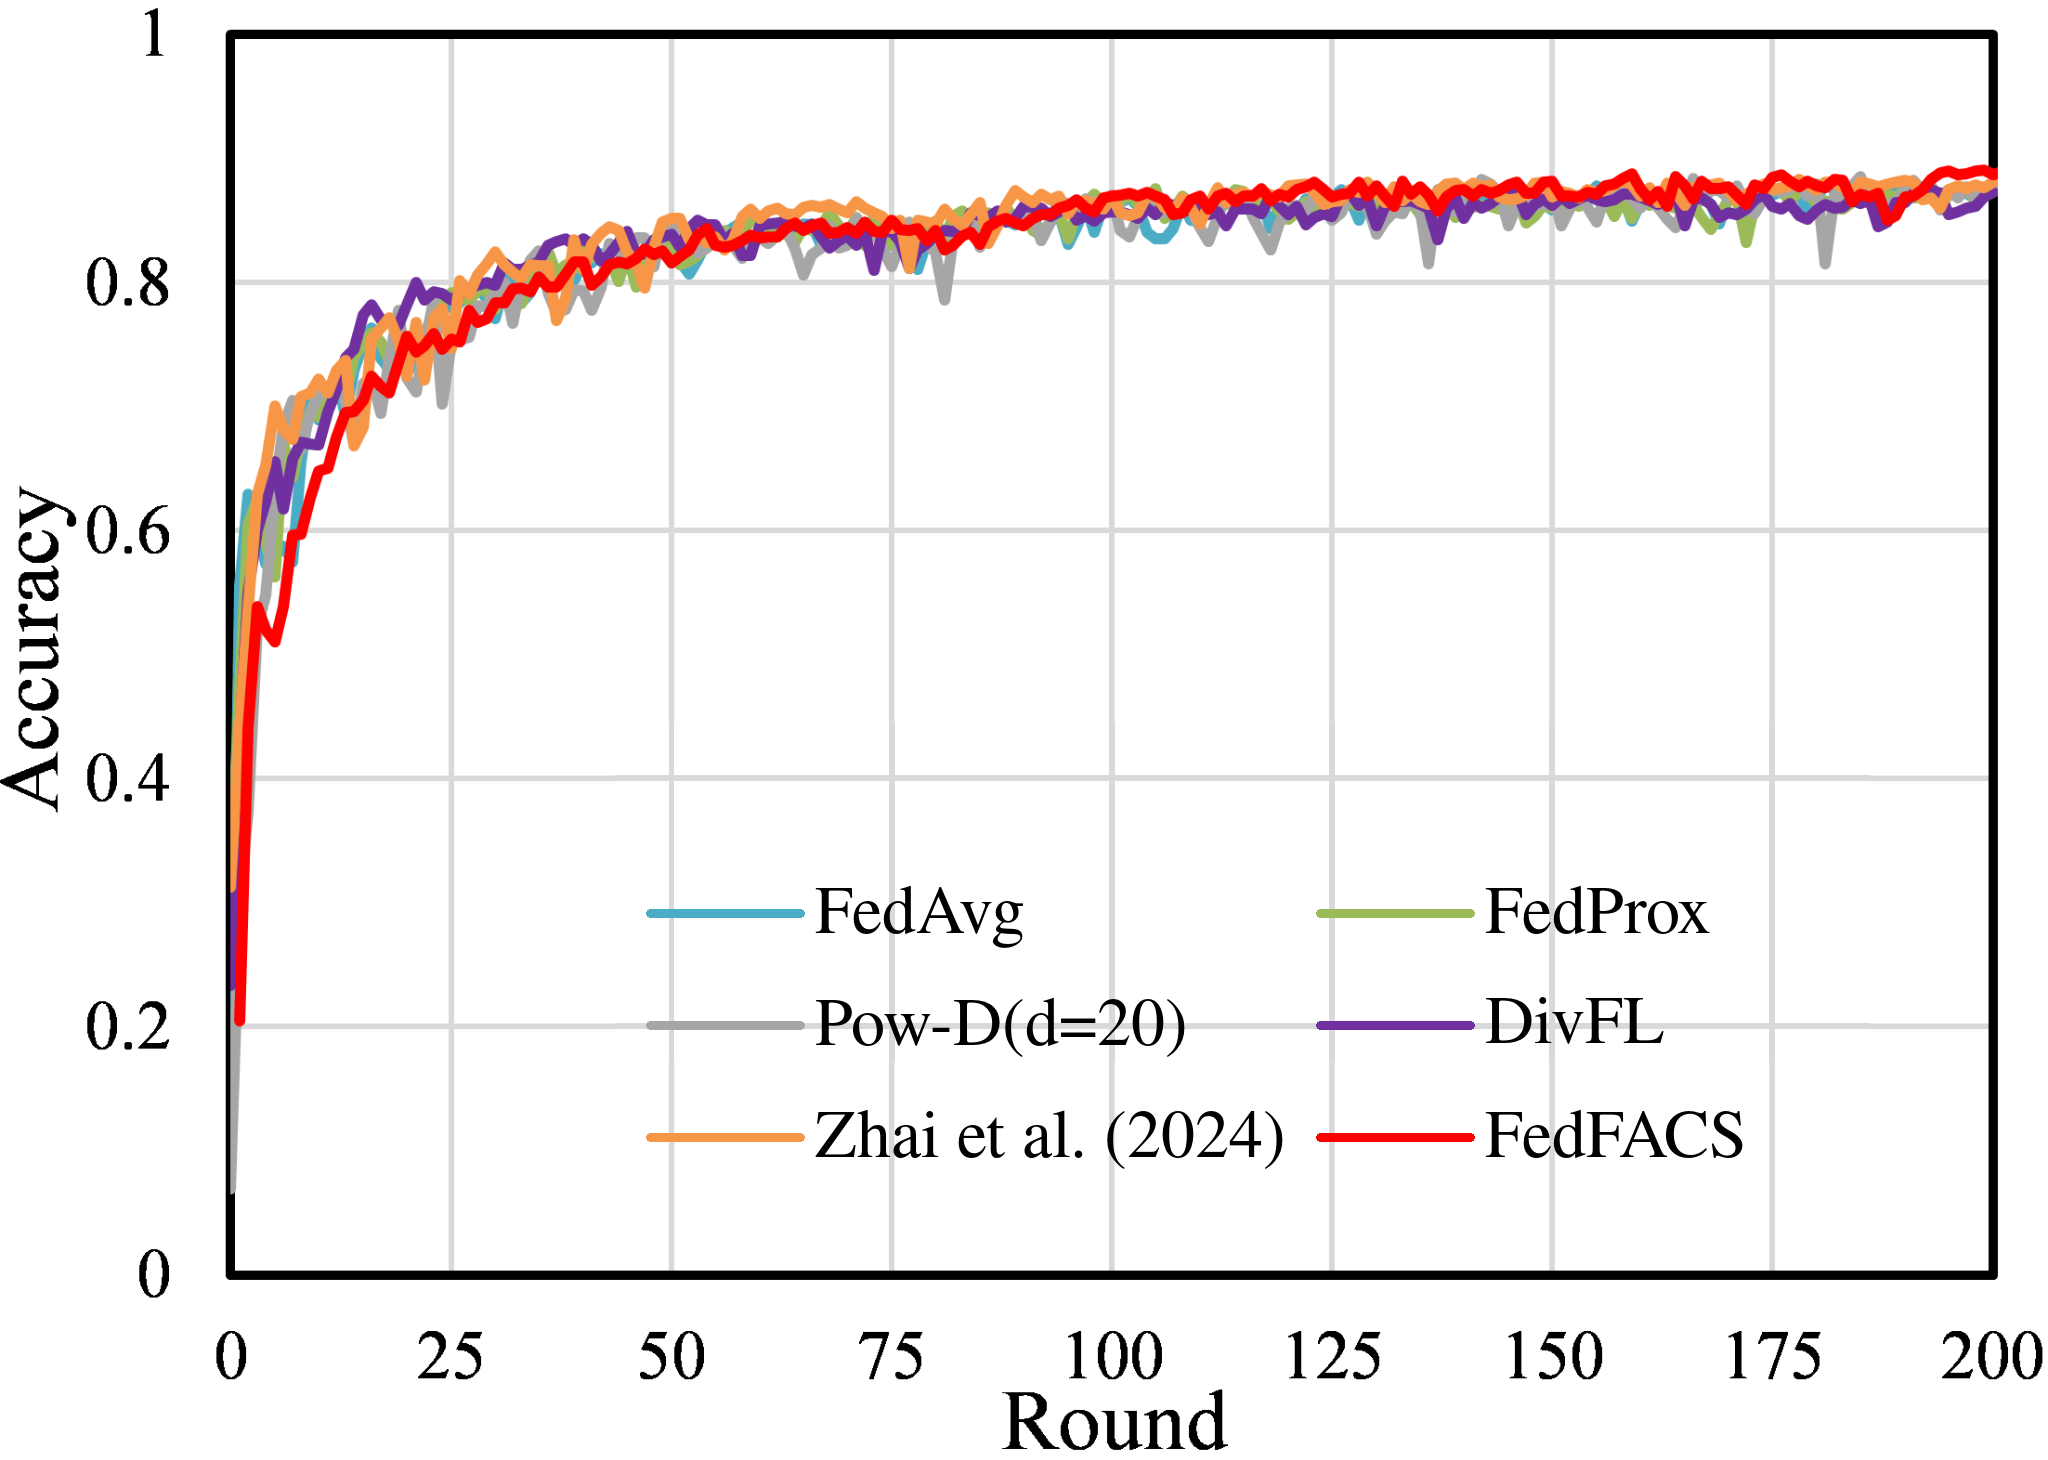
\includegraphics[
        width=\linewidth,
        height=4.15cm,
        keepaspectratio
    ]{figures/fig7__b.png}
    \par\vspace{0.5mm}
    {\fontsize{7pt}{8pt}\selectfont
    (b) Scenario 1 ($\alpha=0.5$)}
\end{minipage}
\hfill
\begin{minipage}[t]{0.32\linewidth}
    \vspace{0pt}\centering
    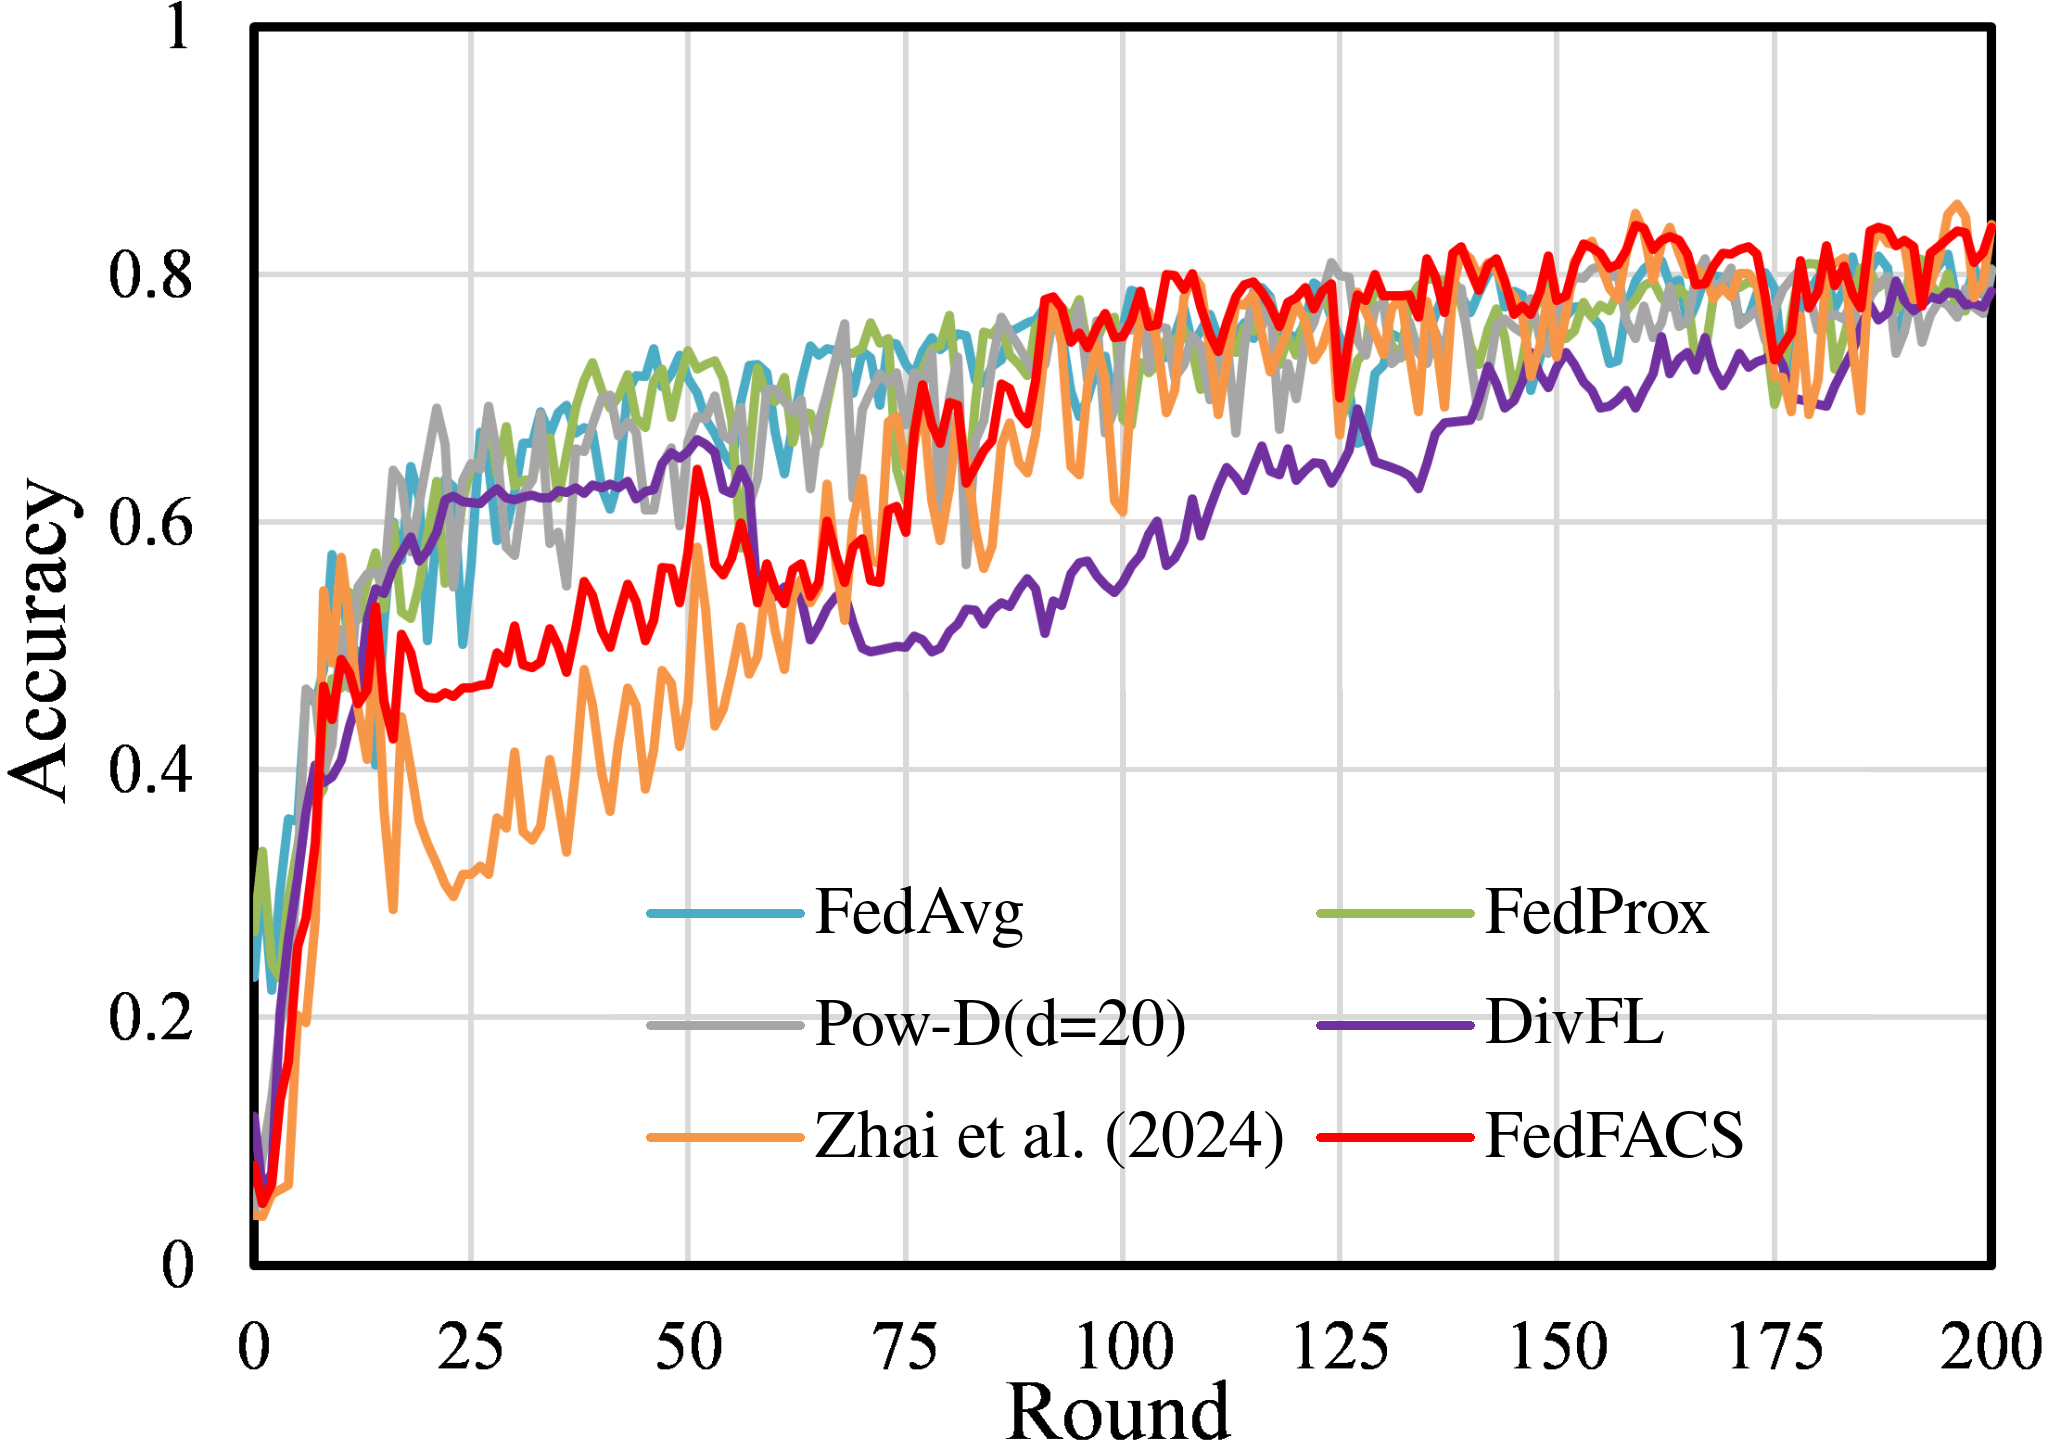
\includegraphics[
        width=\linewidth,
        height=4.15cm,
        keepaspectratio
    ]{figures/fig7__c.png}
    \par\vspace{0.5mm}
    {\fontsize{7pt}{8pt}\selectfont
    (c) Scenario 2}
\end{minipage}

\par\vspace{1mm}

\refstepcounter{figure}

\addcontentsline{lof}{figure}{%
    \protect\numberline{\thefigure}%
    Accuracy comparison under heterogeneous data conditions in Scenarios 1 and 2 on FMNIST.}

{\raggedright
\fontsize{7pt}{8.2pt}\selectfont
\textbf{Fig.~\thefigure}\enspace
Accuracy comparison under heterogeneous data conditions in Scenarios 1 and 2 on FMNIST.
\par}

\end{minipage}

\par\vspace{3mm}

\par\vspace{1mm}

An additional experiment was carried out to further examine the robustness of FedFACS through comparisons with several client selection methods based on predictive accuracy, classification quality, and communication efficiency. Experimental evaluation was performed using FMNIST, CIFAR-10, and COVID-19 to further demonstrate its effectiveness for medical image classification under the first data partitioning scenario (S1) with a Dirichlet parameter of $\alpha = 0.5$, following Configuration B.

As illustrated in Figs. 8 and 9, FedFACS outperforms the baseline approaches across all experimental datasets. On FMNIST, FedFACS achieves an accuracy of 87.1\% improving Random, FedProx, and AHIBCS by 6.74\%, 4.31\%, and 1.40\%, respectively. Similarly, on CIFAR-10, FedFACS achieves an accuracy of 54.3\%, corresponding to improvements of 5.85\%, 10.82\%, and 2.26\% over the baseline methods. Across the FMNIST and CIFAR-10 datasets, FedFACS provides an average relative accuracy improvement of 1.2\% over AHIBCS. For the COVID-19 dataset, FedFACS demonstrates its effectiveness by achieving the highest classification accuracy of 95.3\%, outperforming AHIBCS by 0.5\%. These findings demonstrate that FedFACS successfully selects informative clients while maintaining robust performance under diverse datasets and application domains.   

Table 4 compares the recall and F1-score obtained by the evaluated methods (Liu et al. 2025), showing that FedFACS records the highest F1-score on all considered datasets and demonstrates competitive recall performance, demonstrating more reliable discrimination between classes. Table 5 evaluates communication efficiency by reporting the communication rounds together with the total number of aggregated client participations needed to attain predefined accuracy levels of 83\%, 50\%, and 91\% on FMNIST, CIFAR-10, and COVID-19, respectively. Although AHIBCS requires fewer communication rounds on FMNIST and CIFAR-10, FedFACS achieves better classification performance with a slight increase in number of communication rounds. Specifically, FedFACS requires 35 and 151 rounds on FMNIST and CIFAR-10, respectively, compared with 27 and 144 rounds for AHIBCS. However, adaptive client selection enables FedFACS to reduce communication overhead, resulting in 266 cumulative aggregated client participation on FMNIST and 1381 on CIFAR-10, representing reductions of 1.48\% and 4.10\%, respectively, compared with AHIBCS. On the COVID-19 dataset, FedFACS achieves the target accuracy in 103 rounds, compared with 110 rounds for AHIBCS, representing a 6.36\% reduction in communication rounds with fewer participating clients.


%%%%%%%%%%%%%%%%%%%%%%%%%%%%%%%%%%%%%%%%%%%%%%%%%%%%%%
% Figures 8--9 and Tables 4--5 in One Fixed Block
%%%%%%%%%%%%%%%%%%%%%%%%%%%%%%%%%%%%%%%%%%%%%%%%%%%%%%

\noindent
\begin{minipage}[t]{\linewidth}
\centering

%%%%%%%%%%%%%%%%%%%%%%%%%%%%%%%%%%%%%%%%%%%%%%%%%%%%%%
% Two Images Side by Side
%%%%%%%%%%%%%%%%%%%%%%%%%%%%%%%%%%%%%%%%%%%%%%%%%%%%%%

\noindent
\begin{minipage}[t]{0.485\linewidth}
    \vspace{0pt}
    \centering

    % Fixed image area: identical top and bottom alignment
    \begin{minipage}[t][4.35cm][t]{\linewidth}
        \vspace{0pt}
        \centering
        \resizebox{\linewidth}{4.25cm}{%
            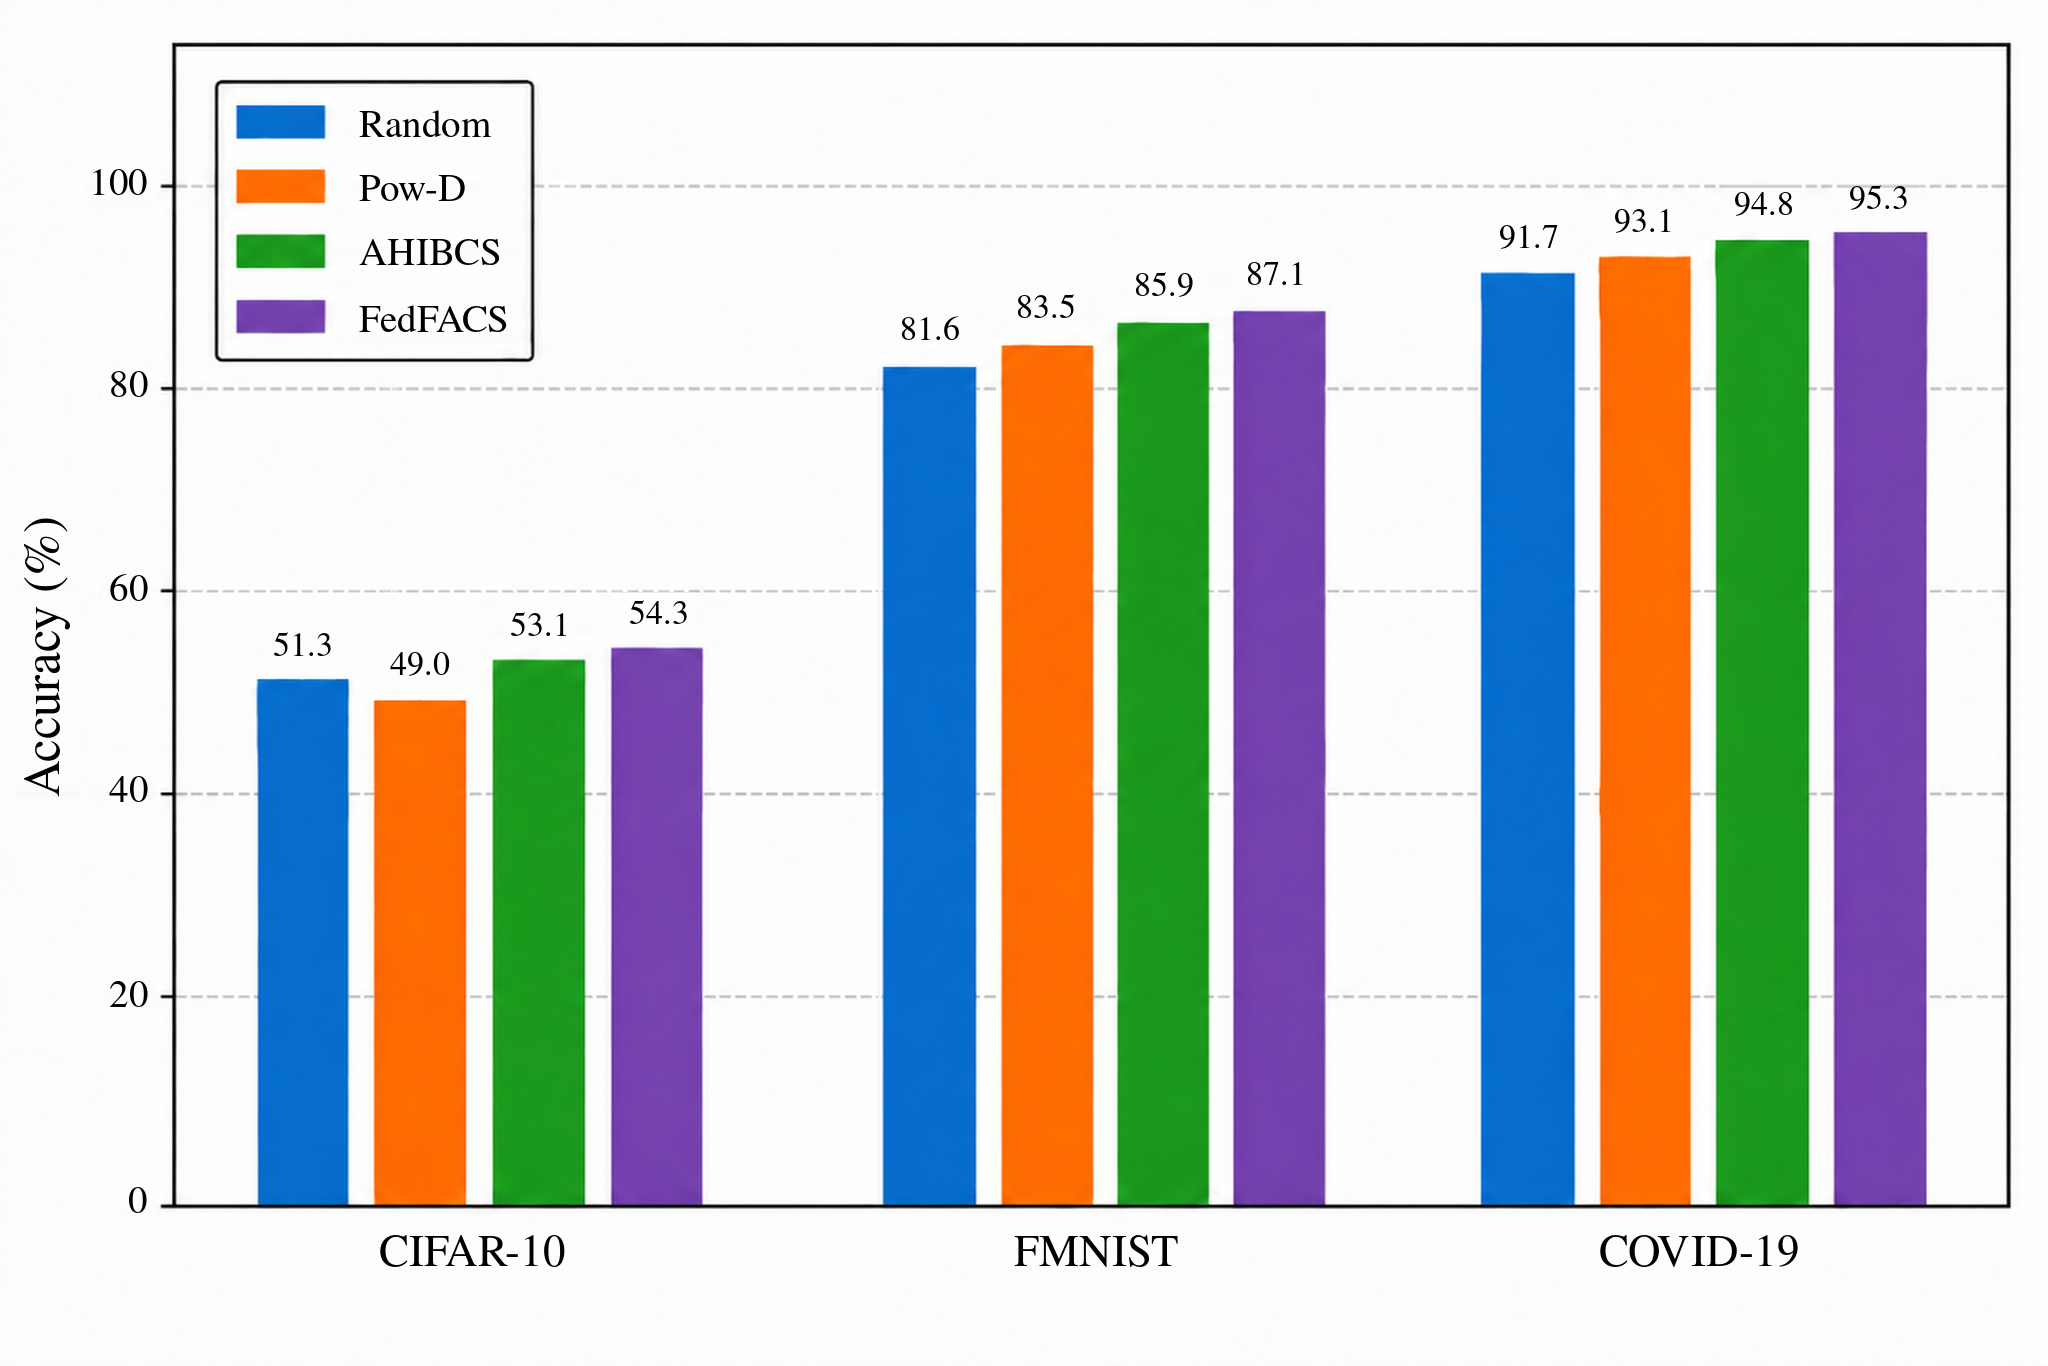
\includegraphics{figures/fig8__bar.png}%
        }
    \end{minipage}

    \par\vspace{-0.5mm}

    \refstepcounter{figure}
    \label{fig:accuracy}

    \parbox[t][0.9cm][t]{\linewidth}{%
        \raggedright
        \fontsize{7pt}{8pt}\selectfont
        \textbf{Fig.~\thefigure}\enspace
        Accuracy comparison of Random, Pow-D, AHIBCS, and FedFACS on multiple benchmark datasets.
    }
\end{minipage}
\hfill
\begin{minipage}[t]{0.485\linewidth}
    \vspace{0pt}
    \centering

    % Fixed image area: identical top and bottom alignment
    \begin{minipage}[t][4.35cm][t]{\linewidth}
        \vspace{0pt}
        \centering
        \resizebox{\linewidth}{4.25cm}{%
            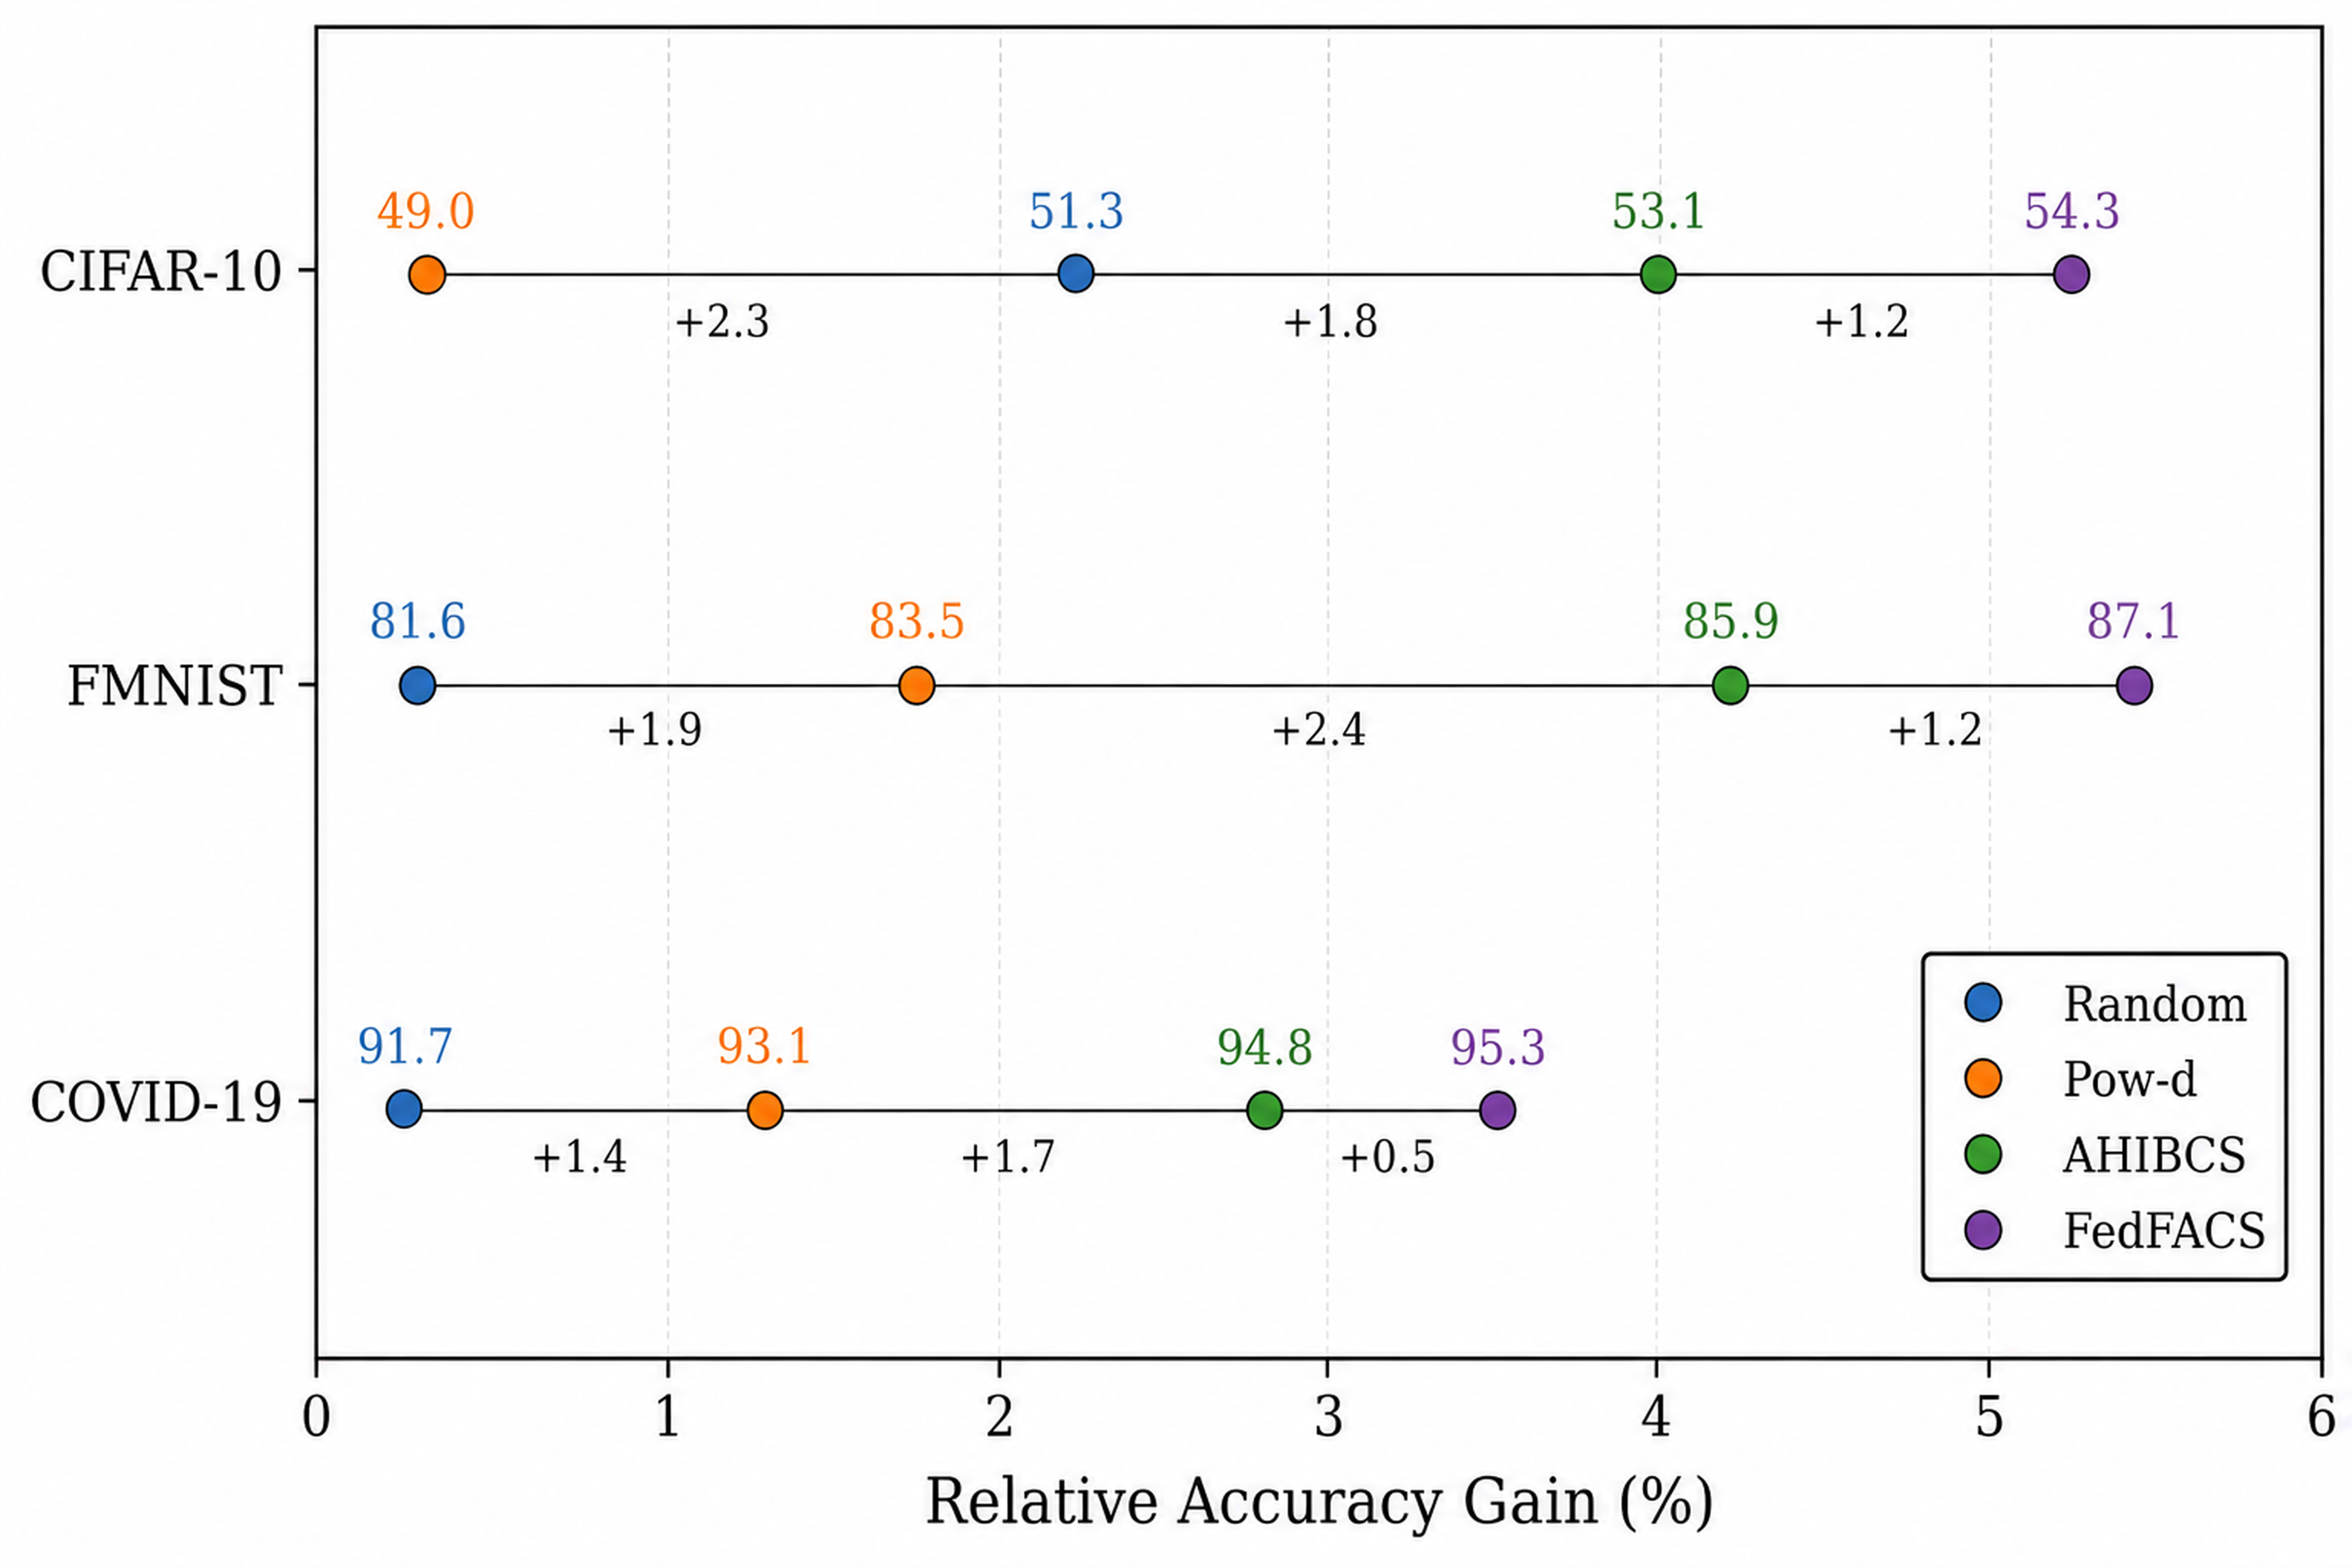
\includegraphics{figures/fig9__relative.png}%
        }
    \end{minipage}

    \par\vspace{-0.5mm}

    \refstepcounter{figure}
    \label{fig:comparison}

    \parbox[t][0.9cm][t]{\linewidth}{%
        \raggedright
        \fontsize{7pt}{8pt}\selectfont
        \textbf{Fig.~\thefigure}\enspace
        Relative accuracy comparison between different client selection models on multiple benchmark datasets.
    }
\end{minipage}

\par\vspace{1.5mm}


%%%%%%%%%%%%%%%%%%%%%%%%%%%%%%%%%%%%%%%%%%%%%%%%%%%%%%
% End of the Outer Block Containing Figures 8--9
%%%%%%%%%%%%%%%%%%%%%%%%%%%%%%%%%%%%%%%%%%%%%%%%%%%%%%

\end{minipage}
% End of the outer fixed block containing Figures 8--9


%%%%%%%%%%%%%%%%%%%%%%%%%%%%%%%%%%%%%%%%%%%%%%%%%%%%%%
% Table 4: Recall and F1-score
%%%%%%%%%%%%%%%%%%%%%%%%%%%%%%%%%%%%%%%%%%%%%%%%%%%%%%

\begin{table}[!htbp]
\centering
\footnotesize
\setlength{\tabcolsep}{4pt}
\renewcommand{\arraystretch}{1.15}
\setlength{\abovecaptionskip}{0pt}
\setlength{\belowcaptionskip}{2pt}

\caption{Comparison of recall and F1-score among various client selection approaches over multiple benchmark dataset.}
\label{tab:recall_f1}

\begin{tabular*}{\journalfloatwidth}{
    @{\extracolsep{\fill}}
    l cc cc cc
    @{}
}
\toprule
Model
& \multicolumn{2}{c}{FMNIST}
& \multicolumn{2}{c}{CIFAR-10}
& \multicolumn{2}{c}{COVID-19} \\
\cmidrule(lr){2-3}
\cmidrule(lr){4-5}
\cmidrule(lr){6-7}
& Recall & F1 Score
& Recall & F1 Score
& Recall & F1 Score \\
\midrule
Random  & 0.815 & 0.861 & 0.471 & 0.569 & 0.921 & 0.919 \\
Pow-D   & 0.838 & 0.882 & 0.449 & 0.547 & 0.926 & 0.934 \\
AHIBCS  & 0.853 & 0.894 & 0.523 & 0.620 & \textbf{0.948} & 0.945 \\
FedFACS & \textbf{0.867} & \textbf{0.907}
        & \textbf{0.529} & \textbf{0.634}
        & 0.934 & \textbf{0.950} \\
\bottomrule
\end{tabular*}

\end{table}
\vspace{-4mm}
%%%%%%%%%%%%%%%%%%%%%%%%%%%%%%%%%%%%%%%%%%%%%%%%%%%%%%
% Table 5: Communication Efficiency
%%%%%%%%%%%%%%%%%%%%%%%%%%%%%%%%%%%%%%%%%%%%%%%%%%%%%%

\begin{table}[!htbp]
\centering
\footnotesize
\setlength{\tabcolsep}{4pt}
\renewcommand{\arraystretch}{1.15}
\setlength{\abovecaptionskip}{0pt}
\setlength{\belowcaptionskip}{2pt}

\caption{Communication rounds and cumulative number of aggregated clients corresponding to predefined accuracy.}
\label{tab:communication}

\begin{tabular*}{\journalfloatwidth}{
    @{\extracolsep{\fill}}
    l cc cc cc
    @{}
}
\toprule
Model
& \multicolumn{2}{c}{FMNIST}
& \multicolumn{2}{c}{CIFAR-10}
& \multicolumn{2}{c}{COVID-19} \\
\cmidrule(lr){2-3}
\cmidrule(lr){4-5}
\cmidrule(lr){6-7}
& Rounds & Clients
& Rounds & Clients
& Rounds & Clients \\
\midrule
Random  & 81 & 810 & 267 & 2670 & 265 & 2650 \\
Pow-D   & 53 & 530 & 198 & 1980 & 183 & 1830 \\
AHIBCS  & \textbf{27} & 270 & \textbf{144} & 1440 & 110 & 1100 \\
FedFACS & 35 & \textbf{266}
        & 151 & \textbf{1381}
        & \textbf{103} & \textbf{1047} \\
\bottomrule
\end{tabular*}

\end{table}

\FloatBarrier

\par\vspace{0.5mm}

This is achieved through the integration of fitness-based client selection, adaptive cohort sizing, and stability-weighted aggregation, which enhance the effectiveness of federated learning under heterogeneous data distributions, facilitate faster convergence, and enable more efficient utilization of participating clients. Consequently, FedFACS is well suited to practical federated learning environments with limited communication resources. 

%%%%%%%%%%%%%%%%%%%%%%%%%%%%%%%%%%%%%%%%%%%%%%%%%%%%%%
% Start this section on a new page
%%%%%%%%%%%%%%%%%%%%%%%%%%%%%%%%%%%%%%%%%%%%%%%%%%%%%%

\FloatBarrier


Further experiments were conducted using multiple benchmark datasets across data partitioning scenarios 3 and 4 with configuration C, focusing on accuracy and fairness relative to the baseline approaches. Table 6 illustrates that FedFACS retains global model accuracy and outperforms FedFairCS under various experimental conditions. The proposed approach prioritizes clients with informative and low uncertainty updates while ensuring fair participation, which improves the convergence.




%% Tables 4 %%
\begin{table}[!htbp]
\centering
\footnotesize
\setlength{\tabcolsep}{4pt}
\renewcommand{\arraystretch}{1.15}
\setlength{\abovecaptionskip}{2pt}
\setlength{\belowcaptionskip}{4pt}

\caption{Accuracy comparison under Scenario~3 and Scenario~4.}
\label{tab:accuracy_s3_s4}

\begin{tabular*}{\journalfloatwidth}{@{\extracolsep{\fill}}llccccc@{}}
\toprule
Dataset & Scenario & Random & Greedy & RBFF & FedFairCS & FedFACS \\
\cmidrule(lr){3-7}
 &  & Acc. (\%) & Acc. (\%) & Acc. (\%) & Acc. (\%) & Acc. (\%) \\
\midrule
CIFAR-10 & S3 & 53.95 & 47.66 & 55.81 & \textbf{56.15} & 55.85 \\
         & S4 (noisy data 10\%) & 51.34 & 44.37 & 53.54 & 53.85 & \textbf{54.21} \\
         & S4 (noisy data 20\%) & 50.31 & 41.78 & 53.38 & 53.43 & \textbf{53.70} \\

FMNIST   & S3 & 86.63 & 85.18 & 86.55 & 87.39 & \textbf{87.48} \\
         & S4 (noisy data 10\%) & 80.52 & 81.54 & 83.19 & 83.16 & \textbf{83.32} \\
         & S4 (noisy data 20\%) & 80.81 & 78.50 & 80.40 & \textbf{83.27} & 83.11 \\
\bottomrule
\end{tabular*}


\end{table}

\begin{figure}[!htbp]
\centering
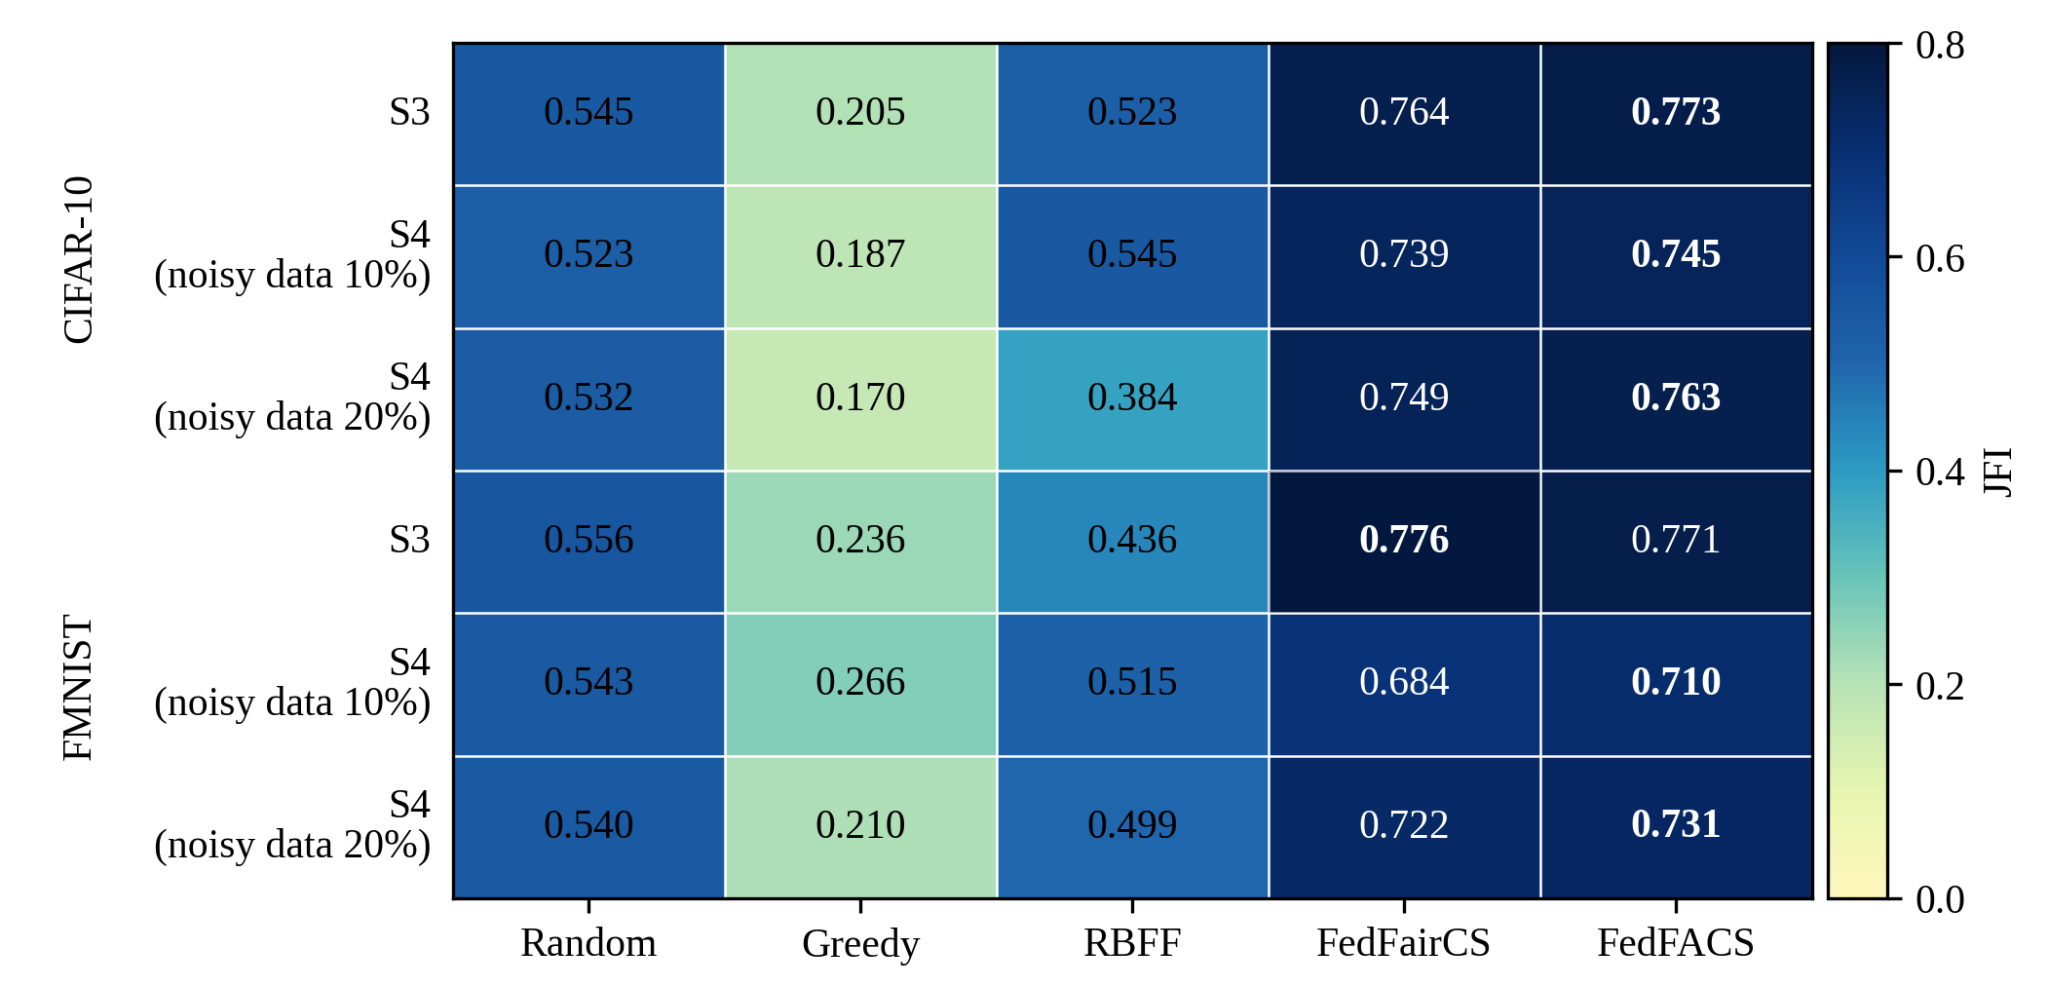
\includegraphics[
    width=0.92\linewidth,
    height=0.34\textheight,
    keepaspectratio
]{figures/fig10__heatmap.png}

\caption{Jain Fairness Index (JFI) comparison under Scenarios 3 and 4 for CIFAR-10 and FMNIST. Darker colors denote higher fairness values.}

\label{fig:jfi_heatmap}
\end{figure}

\begin{figure}[!htbp]
\centering
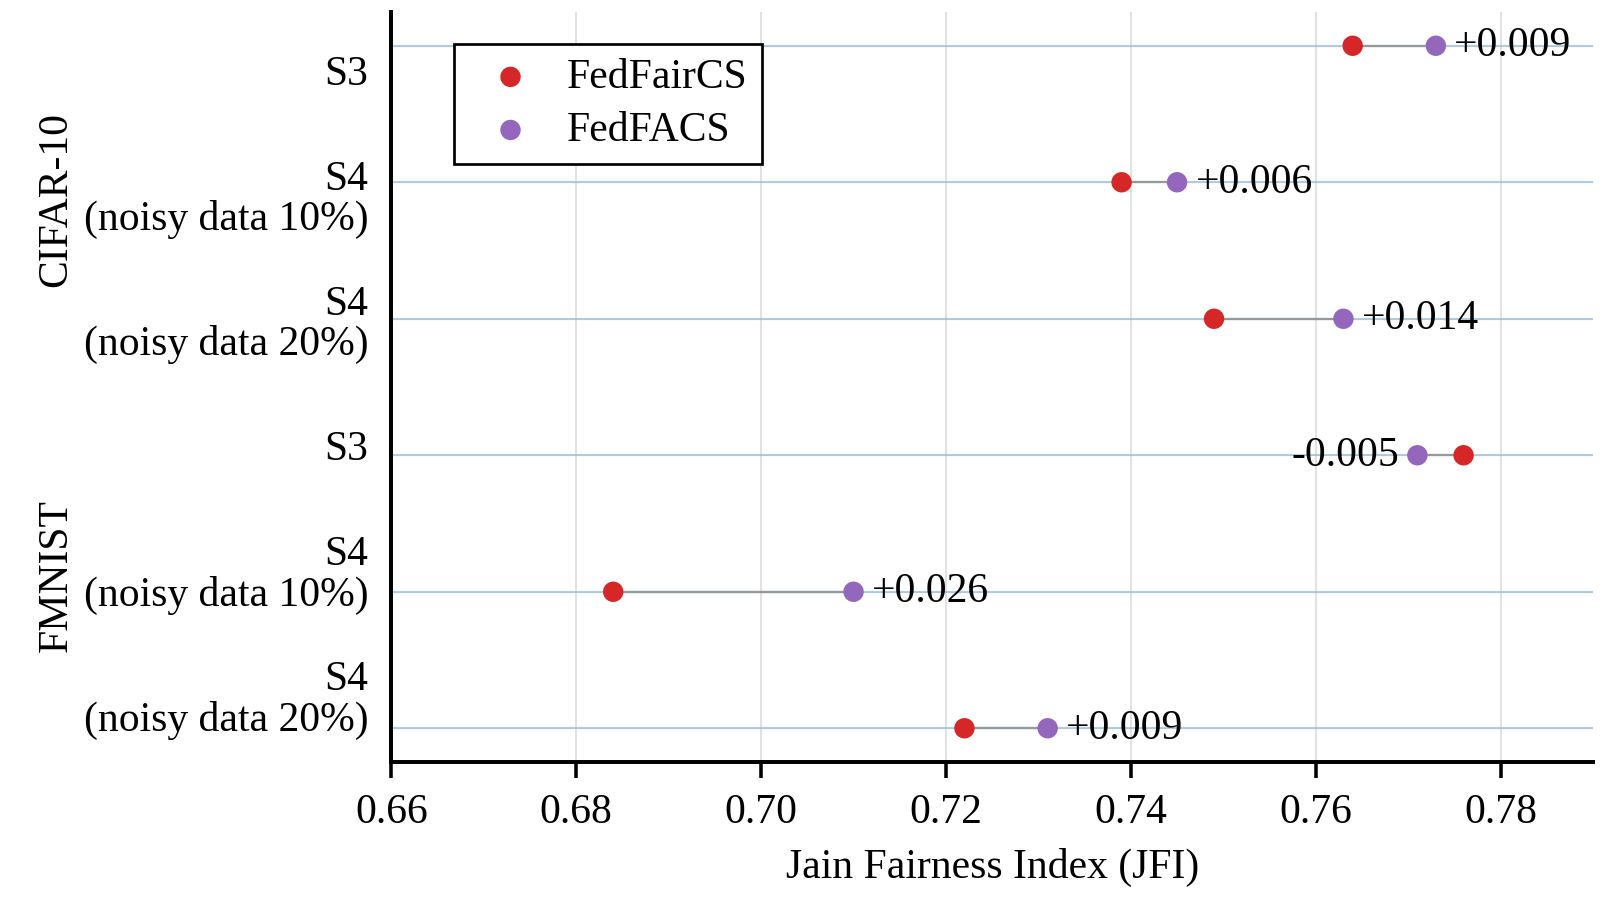
\includegraphics[
    width=0.92\linewidth,
    height=0.34\textheight,
    keepaspectratio
]{figures/fig11__relative.png}

\vspace{1mm}

\caption{JFI comparison between FedFACS and FedFairCS under Scenarios 3 and 4. Each row represents a dataset–scenario condition, where the red point denotes the best baseline method and the purple point indicates FedFACS. The annotated value indicates the signed difference between FedFACS and the best baseline.}
\label{fig:jfi_pairwise_comparison}
\end{figure}


As depicted in Fig.~10, FedFACS improves fairness compared with the best-performing baseline, FedFairCS, achieving average \textit{JFI} improvements of approximately 1.29\% on CIFAR-10 and 1.47\% on FMNIST. FedFACS achieves slightly higher \textit{JFI} values than FedFairCS in most scenarios, with gains ranging from (+0.006) to (+0.026) as shown in Fig. 11. These results indicate that FedFACS can improve fairness under non-IID and noisy-data settings while avoiding fairness degradation. This results indicates fair client participation across training rounds where all clients are selected with varying frequencies according to their impact on the global model performance. Moreover, FedFACS achieves the stated performance with fewer participating clients by using dynamic cohort sizing based on the global model’s convergence state $(C_{k_{\min}} < C_k^t \le m)$ instead of selecting a predefined client sampling size \textit{m} in every communication round as in baseline methods $(m = C_k^t)$. 


Although improving fairness often leads to a degradation of accuracy, the proposed FedFACS effectively manages this trade-off by avoiding forced uniform participation (\textit{JFI}=1), which negatively affects overall model accuracy by limiting contribution from highly informative clients, especially under heterogeneous data distributions. Instead, FedFACS employs an adaptive control mechanism that regulates client selection frequency based on their real-time impact on model convergence. Furthermore, the stability-weighted aggregation strategy improves accuracy by assigning greater weights to updates from more stable clients. This design enables informative clients to participate more frequently while preventing client starvation. Consequently, FedFACS achieves higher fairness while preserving or improving accuracy, with fewer participating clients and reduced communication cost.


Finally, the full FedFACS model improves accuracy, communication efficiency and, fairness by integrating adaptive client selection, dynamic cohort sizing, and adaptive stability-weighted aggregation. This integration leverages the proposed client selection mechanism to fairly identify and select highly effective clients and maximize the effectiveness of informative and stable clients while preserving fair participation for less informative clients. This synergy improves training efficiency by accelerating and stabilizing convergence, showing that each component is crucial for balancing high model accuracy with low communication costs while ensuring fair client participation.

The performance analysis demonstrate that the proposed framework delivers superior results compared with current benchmark methods across different heterogeneous data scenarios on CIFAR-10, MNIST, and FMNIST datasets. Consequently, FedFACS improves global performance, ensures fairness, and reduces the communication overhead by accelerating convergence by achieving target performance with fewer communication rounds and selecting fewer clients.


\FloatBarrier
\section{Conclusion}
\label{sec:conclusion}

This study presents FedFACS, an adaptive and fairness-aware client selection mechanism designed to improve communication efficiency while preserving model accuracy and generalization under heterogeneous data distributions. The proposed framework adapts the client selection strategy according to the convergence performance of the global model, maintaining a balance between informativeness and fairness. Moreover, stability-aware aggregation is employed, assigning higher weights to reliable client updates, thereby enhancing the stability and reliability of the resulting global model. Evaluation results across diverse benchmark datasets under various data partitioning scenarios show that the proposed FedFACS provides higher classification accuracy and speeds up convergence, while selecting the minimum number of clients to reduce communication overhead while preserving fairness in client selection compared with the best-performing baseline methods.

While FedFACS handles data heterogeneity and label noise, its robustness against advanced adversarial attacks and Byzantine participants remains unexplored. Future work will extend the framework by integrating data poisoning attack detection and mitigation mechanisms while supporting complex multimodal datasets for real-world applications.

\FloatBarrier
\backmatter


\section{References}

\begingroup
\small
\setlength{\emergencystretch}{2em}
\setlength{\parindent}{0pt}
\setlength{\parskip}{0pt}
\setlength{\leftskip}{0pt}
\setlength{\rightskip}{0pt}
\Urlmuskip=0mu plus 1mu\relax
\renewcommand{\section}[2]{}

\begin{thebibliography}{99}
\setlength{\itemsep}{3pt}
\setlength{\parsep}{0pt}

\bibitem{ref1}
Ahmed AA, Alabi OO (2024) Secure and Scalable Blockchain-Based Federated Learning for Cryptocurrency Fraud Detection: A Systematic Review. IEEE Access, 12, 102219-102241. \url{https://doi.org/10.1109/ACCESS.2024.3429205}

\bibitem{ref2}
Amini A, Vieira T, Cotterell R (2025) Better estimation of the Kullback–Leibler divergence between language models. In: The Thirty-Ninth Annual Conference on Neural Information Processing Systems. \url{https://doi.org/10.48550/arXiv.2504.10637}

\bibitem{ref3}
Asad M, Shaukat S, Hu D, Wang Z, Javanmardi E, Nakazato J, Tsukada M (2023) Limitations and Future Aspects of Communication Costs in Federated Learning: A Survey. Sensors, 23(17), 7358. \url{https://doi.org/10.3390/s23177358}

\bibitem{ref4}
Ayeelyan J, Utomo S, Rouniyar A et al. (2025) Federated learning design and functional models: survey.  Artificial Intelligence Review 58, 21. \url{https://doi.org/10.1007/s10462-024-10969-y}

\bibitem{ref5}
Balakrishnan R, Li T, Zhou T, Himayat N, Smith V, Bilmes J (2022) Diverse client selection for federated learning via submodular maximization. In: International Conference on Learning Representations (ICLR)

\bibitem{ref6}
Bouzamoucha R, Ktata FB, Zhioua S (2025) Fair client selection in federated learning: enhancing fairness in collaborative AI systems. 14th International Conference on Data Science, Technology and Applications (DATA 2025), pp. 263-273. \url{https://doi.org/10.5220/0013397900003967}

\bibitem{ref7}
Chaudhari M, Andersson G, Hiskens IA. (2002) Control Lyapunov functions for controllable series devices. IEEE Power Engineering Society Winter Meeting. \url{https://doi.org/10.1109/PESW.2002.985105}.

\bibitem{ref8}
Chaudhury BR, Murhekar A, Yuan Z, Li B, Mehta R, Procaccia AD (2024) Fair Federated Learning via the Proportional Veto Core. In 41st International Conference on Machine Learning, 42245-42257

\bibitem{ref9}
Cho YJ, Gupta S, Joshi G, Yağan O. (2020) Bandit-based communication-efficient client selection strategies for federated learning. In: Proceedings of the ACSSC 2020. pp. 1066–1069, \url{https://doi.org/10.1109/IEEECONF51394.2020.9443523}

\bibitem{ref10}
Cho YJ, Wang J, Joshi G (2022) Towards understanding biased client selection in federated learning. In International Conference on Artificial Intelligence and Statistics, pp. 10351–10375. \url{https://proceedings.mlr.press/v151/jee-cho22a.html}. Accessed 25 Sep 2025

\bibitem{ref11}
Darzi E, Sijtsema NM, van Ooijen PMA (2024) A comparative study of federated learning methods for COVID-19 detection. Science Report 14, 3944. \url{https://doi.org/10.1038/s41598-024-54323-2}.

\bibitem{ref12}
Fu L, Zhang H, Gao G, Zhang M, Liu X (2023) Client selection in federated learning: Principles, challenges, and opportunities. IEEE Internet Things Journal., vol. 10(24), 21811–21819 \url{https://doi.org/10.1109/JIOT.2023.3299573}.


\bibitem{ref13}
GlobeNewswire (2024) Federated learning market valuation to reach USD 311.4 billion by 2032, CAGR of 10.2\%. GlobeNewswire News Room. Available at: \url{https://www.globenewswire.com/news-release/2024/01/11/2807710/0/en/Federated-Learning-Market-Valuation-to-Reach-USD-311-4-billion-by-2032-CAGR-of-10-2.html}. Accessed 24 Dec 2025.


\bibitem{ref14}
He K, Zhang X, Ren S, Sun J (2016) Deep residual learning for image recognition. In: 2016 IEEE Conference on Computer Vision and Pattern Recognition (CVPR), pp. 770–778. \url{https://doi.org/10.1109/CVPR.2016.90}

\bibitem{ref15}
Huang T, Lin W, Wu W, He L, Li K, Zomaya AY (2020) An efficiency-boosting client selection scheme for federated learning with fairness guarantee. IEEE Transactions on Parallel and Distributed Systems, 32, 1552–1564. \url{https://doi.org/10.48550/arXiv.2011.01783}

\bibitem{ref16}
Huang W, Ye M, Shi Z, Wan G, Li H, Du B, Yang Q (2024) Federated learning for generalization, robustness, fairness: a survey and benchmark. IEEE Transactions on Pattern Analysis and Machine Intelligence, 46(12), Pages 9387 – 9406. \url{https://doi.org/10.1109/TPAMI.2024.3418862}

\bibitem{ref17}
Iyer VN (2023) A review on different techniques to combat the non-IID and heterogeneous nature of data in federated learning. arXiv:2306.02222 Accessed 17 Dec 2025

\bibitem{ref18}
Ji S, Pan S, Long G, Li X, Jiang J, Huang Z (2019) Learning private neural language modeling with attentive aggregation. In: Proceedings of the International Joint Conference on Neural Networks (IJCNN 2019), pp. 1–8. \url{https://doi.org/10.1109/IJCNN.2019.8852464}

\bibitem{ref19}
Ji X, Tian J, Zhang H, Wu D, Li T (2023). Joint device selection and bandwidth allocation for cost-efficient federated learning in Industrial Internet of Things. IEEE Internet of Things Journal, 10(10), 9148–9160. \url{https://doi.org/10.1109/JIOT.2022.3233595}

\bibitem{ref20}
Kairouz P, McMahan HB, Avent B, Bellet A, Bennis M, Bhagoji NA, et al. (2021) Advances and open problems in federated learning. Foundations and Trends in Machine Learning 14, 1–210. \url{https://doi.org/10.1561/2200000083}

\bibitem{ref21}
Karimireddy SP, Kale S, Mohri M, Reddi S, Stich S, Suresh AT (2020) Scaffold: Stochastic controlled averaging for federated learning. International Conference on Machine Learning (ICML), pp. 5132–5143. \url{https://doi.org/10.48550/arXiv.1910.06378}

\bibitem{ref22}
Khajehali N, Yan J, Chow YW, Fahmideh M (2023) A comprehensive overview of IoT-based federated learning: Focusing on client selection methods, Sensors, 23(16), 7235. \url{https://doi.org/10.3390/s23167235}

\bibitem{ref23}
Khan Y, Sánchez D, Domingo-Ferrer J (2024) Federated learning-based natural language processing: a systematic literature review. Artificial Intelligence Review 57, 57(12), pp. 1-39. \url{https://doi.org/10.1007/s10462-024-10970-5}

\bibitem{ref24}
Krizhevsky A, Hinton G (2009) Learning multiple layers of features from tiny images. Technical report, University of Toronto. \url{https://www.cs.toronto.edu/~kriz/cifar.html}. Accessed 17 Aug 2025

\bibitem{ref25}
Kullback S, Leibler RA (1951) On information and sufficiency. The Annals of Mathematical Statistics, 22(1), pp. 79–86. \url{https://doi.org/10.1214/aoms/1177729694}

\bibitem{ref26}
Lai F, Zhu X, Madhyastha HV, Chowdhury M (2021). Oort: efficient federated learning via guided participant selection. In Proceedings of the 15th USENIX Symposium on Operating Systems Design and Implementation. pp. 19–35. \url{https://doi.org/10.48550/arXiv.2010.06081}.

\bibitem{ref27}
Larsson H, Riaz H, Ickin S (2021). Automated collaborator selection for federated learning with multi-armed bandit agents. In Proceedings of the 4th FlexNets Workshop on Flexible Networks: Artificial Intelligence Supported Network Flexibility and Agility, pp. 44–49. \url{https://doi.org/10.1145/3472735.3473388}

\bibitem{ref28}
LeCun Y, Cortes C, Burges CJC (2010) MNIST handwritten digit database. \url{https://yann.lecun.com/exdb/mnist/}. Accessed 1 Oct 2025

\bibitem{ref29}
Li T, Meng Z, Ni B, Shen J, Wang M (2016) Robust geometric lp-norm feature pooling for image classification and action recognition. Image and Vision Computing 55(2), 64–76. \url{https://doi.org/10.1016/j.imavis.2016.04.002}

\bibitem{ref30}
Li T, Sahu AK, Zaheer M, Sanjabi M, Talwalkar A, Smith V (2020) Federated optimization in heterogeneous networks. Proceedings of Machine Learning and Systems. 2, 429–450. arXiv:1812.06127 Accessed 21 Nov 2022

\bibitem{ref31}
Li C, Zeng X, Zhang M, Cao Z (2022). PyramidFL: a fine-grained client selection framework for efficient federated learning. In Proceedings of ACM MobiCom, pp. 158-171. \url{https://doi.org/10.1145/3495243.3517017}

\bibitem{ref32}
Li Q, Li X, Zhou L, Yan X (2024) AdaFL: Adaptive client selection and dynamic contribution evaluation for efficient federated learning. IEEE International Conference on Acoustics, Speech and Signal Processing (ICASSP), pp. 6645–6649. \url{https://doi.org/10.1109/ICASSP48485.2024.10447356}

\bibitem{ref33}
Liu W, Wang X, Wang B, et al. (2025) AHIBCS: an adaptive historical-information-based client selection algorithm for Non-IID data. Cluster Comput. 28(16). \url{https://doi.org/10.1007/s10586-025-05755-6}

\bibitem{ref34}
Mayhoub SM, Shami TA (2024) Review of Client Selection Methods in Federated Learning. Archives of Computational Methods in Engineering 31(2), 1129–1152. \url{https://doi.org/10.1007/s11831-023-10011-4}

\bibitem{ref35}
McMahan HB, Moore E, Ramage D, Hampson S, Arcas BA (2017) Communication-efficient learning of deep networks from decentralized data. 20th International Conference on Artificial Intelligence and Statistics, pp. 1273–1282. \url{https://doi.org/10.48550/arXiv.1602.05629}

\bibitem{ref36}
Mukhtiar N (2025) A fairer client selection framework for federated Internet of Things: equality, equity, and trade-off perspectives. Companion Proceedings of the ACM on Web Conference 2025 (WWW ’25), pp. 713–716. \url{https://doi.org/10.1145/3701716.3715278}

\bibitem{ref37}
Mukhtiar N, Mahmood A, Sheng QZ (2025) Fairness in federated learning: trends, challenges, and opportunities. Artificial Intelligence for Science and Engineering, 7(6). \url{https://doi.org/10.1002/aisy.202400836}

\bibitem{ref38}
Nishio T, Yonetani R (2019). Client selection for federated learning with heterogeneous resources in mobile edge. IEEE International Conference on Communications, pp. 1–7. arXiv:1804.08333 Accessed 11 Oct 2025

\bibitem{ref39}
Reddi S, Charles Z, Zaheer M, Garrett Z, Rush D, Konečný J, Kumar S, McMahan HB (2021). Adaptive Federated Optimization. International Conference on Learning Representations (ICLR). \url{https://doi.org/10.48550/arXiv.2003.00295}

\bibitem{ref40}
Rahman T, et al. (2020). COVID-19 Radiography Database. Kaggle. Available at: \url{https://www.kaggle.com/datasets/tawsifurrahman/covid19-radiography-database} Accessed 1 Jul 2026.

\bibitem{ref41}
Shanmugarasa Y, Paik Hy, Kanhere SS, et al. (2023) A systematic review of federated learning from clients’ perspective: challenges and solutions. Artificial Intelligence Review 56 (Suppl 2), 1773–1827. \url{https://doi.org/10.1007/s10462-023-10563-8}

\bibitem{ref42}
Shi Y, Liu Z, Shi Z, Yu H (2023) Fairness-Aware Client Selection for Federated Learning. IEEE International Conference on Multimedia and Expo (ICME), pp. 324-329. \url{https://doi.org/10.1109/ICME55011.2023.00063}

\bibitem{ref43}
Shi Y, Yu H, Leung C, (2024) Towards Fairness-Aware Federated Learning. IEEE Transactions on Neural Networks and Learning Systems, 35(9), pp. 11922-11938. \url{https://doi.org/10.1109/TNNLS.2023.3263594}.

\bibitem{ref44}
Song Z, Sun H, Howard HY, Wang X, Zhang Y, Quek TQS (2022) Reputation-Based Federated Learning for Secure Wireless Networks. In IEEE Internet of Things Journal, 9(2), pp. 1212-1226, \url{https://doi.org/10.1109/JIOT.2021.3079104}

\bibitem{ref45}
Tang M, Ning X, Wang Y, Wang Y, Chen Y (2021) FedGP: correlation-based active client selection for heterogeneous federated learning. \url{https://api.semanticscholar.org/CorpusID:260437183} Accessed 11 Oct 2025

\bibitem{ref46}
Tsouvalas V, Saeed A, Ozcelebi T, Meratnia N (2024) Communication- efficient federated learning through adaptive weight clustering and server-side distillation. IEEE International Conference on Acoustics, Speech and Signal Processing (ICASSP), pp. 5805–5809. \url{https://doi.org/10.1109/ICASSP48485.2024.10447174}

\bibitem{ref47}
Vanthang D et al. (2025) A Framework Integrating Federated Learning and Fog Computing Based on Client Sampling and Dynamic Thresholding Techniques. In IEEE Access, 13, pp. 95019-95033. \url{https://doi.org/10.1109/ACCESS.2025.3571979}

\bibitem{ref48}
Vucinich S, Zhu Q (2023). The current state and challenges of fairness in federated learning. IEEE Access 11, pp. 80903–80914. \url{https://doi.org/10.1109/ACCESS.2023.3295412}

\bibitem{ref49}
Wang J, Liu Q, Liang H, Joshi G, Poor HV (2020) Tackling the Objective Inconsistency Problem in Heterogeneous Federated Optimization. 4th Conference on Neural Information Processing Systems (NeurIPS), 33, 7611–7623. \url{https://doi.org/10.48550/arXiv.2007.07481}

\bibitem{ref50}
Wang L, Wang Z, Tang X (2023) Fedeba+: Towards fair and effective federated learning via entropy-based model. arXiv:2301.12407 Accessed 18 Dec 2025

\bibitem{ref51}
Wen J, Zhang Z, Lan Y, et al. (2023) A survey on federated learning: challenges and applications. International journal machine learning and Cyber security 14, 513–535. \url{https://doi.org/10.1007/s13042-022-01647-y}

\bibitem{ref52}
Wu H, Wang P (2021) Fast-convergent federated learning with adaptive weighting. In: Proceedings of the IEEE International Conference on Communications, pp. 1–6. \url{https://doi.org/10.1109/ICC42927.2021.9500890}

\bibitem{ref53}
Xiao H, Rasul K, Vollgraf R (2017) Fashion-MNIST: a novel image dataset for benchmarking machine learning algorithms. arXiv:1708.07747. \url{https://github.com/zalandoresearch/fashion-mnist}. Accessed 21 Oct 2025

\bibitem{ref54}
Xu Y, Xiao MJ, Wu C et al. (2024) Age-of-Information-Aware Federated Learning. Journal of Computer Science and Technology, 39(3), 637–653. \url{https://doi.org/10.1007/s11390-024-3914-x}

\bibitem{ref55}
Yacouby R, Axman D (2020) Probabilistic extension of precision, recall, and F1 score for more thorough evaluation of classification models. In: Proceedings of the first workshop on evaluation and comparison of NLP systems, pp 79–91. \url{https://doi.org/10.18653/v1/2020.eval4nlp-1.9}

\bibitem{ref56}
Ye W, An X, Wang J, Yan X, Carle G (2025) FedABC: Attention-based client selection for federated learning with long-term view. In: Proceedings of the IEEE International Conference on Communications (ICC 2025), pp 801–806. \url{https://doi.org/10.1109/ICC52391.2025.11161564}

\bibitem{ref57}
Zhai R, Jin H, Gong W et al. (2024) Adaptive client selection and model aggregation for heterogeneous federated learning. Multimedia Systems 30, 211 (2024). \url{https://doi.org/10.1007/s00530-024-01386-w}

\bibitem{ref58}
Zhang W, Weiss JC, Zhou S, Walsh T (2022) Fairness amidst non-IID graph data: a literature review. \url{https://doi.org/10.48550/arXiv:2202.07170}

\end{thebibliography}

    



\endgroup


\end{document}